% Options for packages loaded elsewhere
\PassOptionsToPackage{unicode}{hyperref}
\PassOptionsToPackage{hyphens}{url}
%
\documentclass[
  a4paper,
  DIV=11,
  numbers=noendperiod,
  listof=totoc]{scrreprt}

\usepackage{amsmath,amssymb}
\usepackage{setspace}
\usepackage{iftex}
\ifPDFTeX
  \usepackage[T1]{fontenc}
  \usepackage[utf8]{inputenc}
  \usepackage{textcomp} % provide euro and other symbols
\else % if luatex or xetex
  \usepackage{unicode-math}
  \defaultfontfeatures{Scale=MatchLowercase}
  \defaultfontfeatures[\rmfamily]{Ligatures=TeX,Scale=1}
\fi
\usepackage{lmodern}
\ifPDFTeX\else  
    % xetex/luatex font selection
\fi
% Use upquote if available, for straight quotes in verbatim environments
\IfFileExists{upquote.sty}{\usepackage{upquote}}{}
\IfFileExists{microtype.sty}{% use microtype if available
  \usepackage[]{microtype}
  \UseMicrotypeSet[protrusion]{basicmath} % disable protrusion for tt fonts
}{}
\usepackage{xcolor}
\usepackage[top=35mm,left=25mm,heightrounded]{geometry}
\setlength{\emergencystretch}{3em} % prevent overfull lines
\setcounter{secnumdepth}{5}
% Make \paragraph and \subparagraph free-standing
\ifx\paragraph\undefined\else
  \let\oldparagraph\paragraph
  \renewcommand{\paragraph}[1]{\oldparagraph{#1}\mbox{}}
\fi
\ifx\subparagraph\undefined\else
  \let\oldsubparagraph\subparagraph
  \renewcommand{\subparagraph}[1]{\oldsubparagraph{#1}\mbox{}}
\fi


\providecommand{\tightlist}{%
  \setlength{\itemsep}{0pt}\setlength{\parskip}{0pt}}\usepackage{longtable,booktabs,array}
\usepackage{calc} % for calculating minipage widths
% Correct order of tables after \paragraph or \subparagraph
\usepackage{etoolbox}
\makeatletter
\patchcmd\longtable{\par}{\if@noskipsec\mbox{}\fi\par}{}{}
\makeatother
% Allow footnotes in longtable head/foot
\IfFileExists{footnotehyper.sty}{\usepackage{footnotehyper}}{\usepackage{footnote}}
\makesavenoteenv{longtable}
\usepackage{graphicx}
\makeatletter
\def\maxwidth{\ifdim\Gin@nat@width>\linewidth\linewidth\else\Gin@nat@width\fi}
\def\maxheight{\ifdim\Gin@nat@height>\textheight\textheight\else\Gin@nat@height\fi}
\makeatother
% Scale images if necessary, so that they will not overflow the page
% margins by default, and it is still possible to overwrite the defaults
% using explicit options in \includegraphics[width, height, ...]{}
\setkeys{Gin}{width=\maxwidth,height=\maxheight,keepaspectratio}
% Set default figure placement to htbp
\makeatletter
\def\fps@figure{htbp}
\makeatother

\KOMAoption{captions}{tableheading}
\usepackage{setspace}
\usepackage{libertine}
\usepackage[font=small, labelfont=bf, justification=justified, singlelinecheck=true]{caption}
\counterwithout{figure}{chapter}
\counterwithout{figure}{section}
\counterwithout{table}{chapter}
\counterwithout{table}{section}
\usepackage[authordate,backend=biber, doi=false, isbn=false]{biblatex-chicago}
\usepackage[french]{babel}
\usepackage{bookmark}
\setcounter{tocdepth}{4}
\unimathsetup{math-style=french}
\usepackage{acronym}
\usepackage{amsmath}
\usepackage{etoolbox}
\makeatletter
\newif\if@in@acrolist
\AtBeginEnvironment{acronym}{\@in@acrolisttrue}
\newrobustcmd{\LU}[2]{\if@in@acrolist#1\else#2\fi}
\newcommand{\ACF}[1]{{\@in@acrolisttrue\acf{#1}}}
\usepackage{pdflscape}
\usepackage{makecell}
\usepackage{multirow}
\usepackage{booktabs}
\usepackage{graphicx}
\usepackage{subcaption}
\usepackage[capitalise, noabbrev, nameinlink]{cleveref}
\crefdefaultlabelformat{#2\textbf{#1}#3}
\crefformat{subfigure}{#2\textbf{#1}#3}
\crefname{table}{\textbf{table}}{\textbf{tables}}
\Crefname{table}{\textbf{Table}}{\textbf{Tables}}
\crefname{figure}{\textbf{figure}}{\textbf{figures}}
\Crefname{figure}{\textbf{Figure}}{\textbf{Figures}}
\crefname{subfigure}{\textbf{figure}}{\textbf{figures}}
\Crefname{subfigure}{\textbf{Figure}}{\textbf{Figures}}
\renewcommand{\thesubfigure}{\Alph{subfigure}}
\AtEveryBibitem{\clearfield{note}}
\makeatletter
\@ifpackageloaded{caption}{}{\usepackage{caption}}
\AtBeginDocument{%
\ifdefined\contentsname
  \renewcommand*\contentsname{Table of contents}
\else
  \newcommand\contentsname{Table of contents}
\fi
\ifdefined\listfigurename
  \renewcommand*\listfigurename{Liste des Figures}
\else
  \newcommand\listfigurename{Liste des Figures}
\fi
\ifdefined\listtablename
  \renewcommand*\listtablename{Liste des Tables}
\else
  \newcommand\listtablename{Liste des Tables}
\fi
\ifdefined\figurename
  \renewcommand*\figurename{Figure}
\else
  \newcommand\figurename{Figure}
\fi
\ifdefined\tablename
  \renewcommand*\tablename{Table}
\else
  \newcommand\tablename{Table}
\fi
}
\@ifpackageloaded{float}{}{\usepackage{float}}
\floatstyle{ruled}
\@ifundefined{c@chapter}{\newfloat{codelisting}{h}{lop}}{\newfloat{codelisting}{h}{lop}[chapter]}
\floatname{codelisting}{Listing}
\newcommand*\listoflistings{\listof{codelisting}{List of Listings}}
\makeatother
\makeatletter
\makeatother
\makeatletter
\@ifpackageloaded{caption}{}{\usepackage{caption}}
\@ifpackageloaded{subcaption}{}{\usepackage{subcaption}}
\makeatother
\ifLuaTeX
  \usepackage{selnolig}  % disable illegal ligatures
\fi
\usepackage[]{biblatex}
\addbibresource{bibliography/vitamin-d.bib}
\addbibresource{bibliography/organization.bib}
\addbibresource{bibliography/manual.bib}
\usepackage{bookmark}

\IfFileExists{xurl.sty}{\usepackage{xurl}}{} % add URL line breaks if available
\urlstyle{same} % disable monospaced font for URLs
\hypersetup{
  hidelinks,
  pdfcreator={LaTeX via pandoc}}

\author{}
\date{}

\begin{document}


\begin{centering}
\setstretch{1.5} %linestretch is 1.5 in YAML but hasn't registered in this .tex
\large

UNIVERSITE PARIS CITE

FACULTE DES SCIENCES PHARMACEUTIQUES ET BIOLOGIQUES

\vspace{1 cm}

Année 2023 \hfill \hfill N°

\vspace{2cm}
THESE

\vspace{1cm} \Large \textbf{Pour l'obtention du diplôme d'Etat de DOCTEUR EN PHARMACIE Présentée et soutenue publiquement}


\Large \textbf {Vitamine D et COVID-19} \vspace{2 cm}

\large Par \vspace{0.5 cm}

\Large \textbf{HUYNH Minh-Anh} \vspace{1 cm}

\large Sous la direction du Pr. Jean-Pascal De Bandt

\today

\end{centering}
\pagenumbering{gobble}
\clearpage

\setstretch{1.5}
\chapter*{Remerciements}\label{remerciements}

\pagenumbering{gobble}

\newpage{}

% From package bookmark
\renewcommand{\contentsname}{Table des Matières}
\pdfbookmark[section]{\contentsname}{toc}
\tableofcontents{}
\newpage

% Use the following command to rename the lof with latex :
% \renewcommand*\listfigurename{Liste des Figures}
% However, with Quarto and Pandoc, we could use "lof-title"in "crossref: in the YAML"
\listoffigures
\newpage

% \renewcommand*\listtablename{Liste des Tables}
\listoftables

\newpage{}

\chapter*{Liste des Acronymes}\label{liste-des-acronymes}
\addcontentsline{toc}{chapter}{Liste des Acronymes}

\begin{acronym}
\acro{1,24,25(OH)3D3}[1,24,25(OH)\textsubscript{3}D\textsubscript{3}]{1,24,25‐trihydroxycholécalciférol}
\acro{1,25(OH)2D3}[1,25(OH)\textsubscript{2}D\textsubscript{3}]{1,25-dihydroxycholécalciférol\acroextra{ (calcitriol)}}
\acro{7-DHC}{7-déhydrocholestérol}
\acro{24,25(OH)2D3}[24,25(OH)\textsubscript{2}D\textsubscript{3}]{24,25-dihydroxycholécalciférol}
\acro{25(OH)D3}[25(OH)D\textsubscript{3}]{25-hydroxycholécalciferol\acroextra{ (calcidiol ou calcifédiol)}}
\acro{ACE2}{enzyme de conversion de l'angiotensine 2}
\acro{ADN}{acide désoxyribonucléique}
\acro{AJR}{\LU{A}{a}pport \LU{J}{j}ournalier \LU{R}{r}ecommandé}
\acro{ANSES}{Agence Nationale de Sécurité sanitaire de l'alimentation, de l'Environnement et du Travail}
\acro{ANSM}{Agence Nationale de Sécurité des Médicaments}
\acro{CCR10}{C-C chemokine receptor type 10}
\acro{CD}{cluster de différenciation}
\acro{CIVD}{coagulation intravasculaire disséminée}
\acro{Cmax}[C\textsubscript{max}]{concentration maximale}
\acro{CMH-II}{\LU{C}{c}omplexe \LU{M}{m}ajeur d'\LU{H}{h}istocompatibilité de \LU{C}{c}lasse II}
\acro{COVID-19}{Coronavirus Disease 2019}
\acro{CPA}{cellules présentatrices d'antigènes}
\acro{CRS}{cytokine release syndrome}
\acro{CYP24A1}{24-hydroxylase}
\acro{CYP27B1}{25-hydroxyvitamine D\textsubscript{3}-1α-hydroxylase}
\acro{DBP}{vitamin D binding protein}
\acro{EFSA}{European Food Safety Authority}
\acro{eNOS}{endothelial nitric oxide synthase}
\acro{FDA}{Food and Drugs Administration}
\acro{FGF23}{fibroblast growth factor 23}
\acro{IFN-1}{interférons de type I}
\acro{ifna}[IFN-α]{interféron alpha}
\acro{ifng}[IFN-γ]{interféron gamma}
\acro{IKBa}[IκBα]{inhibitor of nuclear factor kappa-b alpha}
\acro{IKKb}[IKKβ]{IkappaB kinase beta}
\acro{IL-2}{interleukine-2}
\acro{IL-4}{interleukine-4}
\acro{IL-6}{interleukine-6}
\acro{IL-8}{interleukine-8}
\acro{IL-10}{interleukine-10}
\acro{IL-12}{interleukine-12}
\acro{IL-17}{interleukine-17}
\acro{IMC}{indice de masse corporelle}
\acro{iNKT}{invariant NK T cell}
\acro{IOM}{Institute of Medicine}
\acro{LOAEL}{Lowest Observed Adverse Effect Level}
\acro{LPS}{lipopolysaccharide}
\acro{nfkb}[NF-κB]{nuclear factor-kappa B}
\acro{NK}{lymphocyte natural killer}
\acro{NO}{oxyde nitrique}
\acro{NOAEL}{Non Observed Adverse Effect Level}
\acro{NOD2}{Nucleotide-binding oligomerization domain-containing protein 2}
\acro{PRR}{pattern recognition receptor}
\acro{PTH}{parathormone}
\acro{RCT}{randomized control trial}
\acro{RXR}{retinoid X receptor}
\acro{SARS-CoV-2}{Severe Acute Respiratory Syndrome Coronavirus 2}
\acro{SDRA}{syndrome de détresse respiratoire aiguë}
\acro{SRAA}{système rénine angiotensine aldostérone}
\acro{TCR}{T cell receptor}
\acro{Th}[T helpers]{lymphocytes T helpers}
\acro{Th1}[Th1]{CD4\textsuperscript{+} type 1 helper T cells}
\acro{Th2}[Th2]{CD4\textsuperscript{+} type 2 helper T cells}
\acro{Th17}[Th17]{CD4\textsuperscript{+} type 17 helper T cells}
\acro{TLR}{toll-like receptor}
\acro{Tmax}[T\textsubscript{max}]{temps auquel la C\textsubscript{max} est atteinte}
\acro{tnfa}[TNF-\mupalpha]{tumor necrosis factor alpha}
\acro{Treg}[T\textsubscript{reg}]{lymphocytes T régulateurs}
\acro{TSA}{trial sequencing analysis}
\acro{UI}{unité internationale}
\acro{VDR}{vitamin D receptor}
\acro{VDRE}{\LU{V}{v}itamin D \LU{R}{r}esponse \LU{E}{e}lement}
\end{acronym}

\newpage{}

\pagenumbering{arabic}

\chapter{Introduction}\label{introduction}

\newpage{}

\chapter{Généralités sur la vitamine
D}\label{guxe9nuxe9ralituxe9s-sur-la-vitamine-d}

\section{Structure}\label{structure}

La vitamine D est un nutriment vital, nécessaire pour notre métabolisme.
Elle possède un rôle de vitamine qui est définie comme étant une
substance organique essentielle en quantités infimes, à la nutrition de
la plupart des animaux et de certaines plantes. La plupart des vitamines
agissent comme coenzymes et précurseurs de coenzymes pour réguler les
processus métaboliques mais ne fournissent pas d'énergie et ne servent
pas d'unités de construction \autocite{Ellison.2021} ; la vitamine D
intervient comme précurseur d'une hormone, le calcitriol.

La vitamine D est une molécule liposoluble dérivée du cholestérol et se
distinguant des hormones stéroïdes par l'ouverture du cycle B de la
structure cyclopentanoperhydrophénanthrène \autocite{Norman.2008}
(\Cref{fig:vitd3}). Il en existe deux formes, la vitamine
D\textsubscript{2} ou ergocalciférol, synthétisée par les plantes et
champignons, et la vitamine D\textsubscript{3} ou cholécalciférol,
synthétisée dans la peau après une exposition aux rayons ultraviolets B
ou à la lumière du soleil. A la différence des autres vitamines, la
vitamine D peut donc être synthétisée par l'organisme humain, mais en
quantité insuffisante par rapport aux besoins, d'où l'impérative
nécessité d'un apport exogène. Généralement, les termes vitamine D fait
référence à la vitamine D\textsubscript{3}. Pour être active, la
vitamine D doit subir une double hydroxylation en positions 1 et 25,
formant ainsi une hormone, le calcitriol ou
1,25-dihydroxycholécalciférol. Le calcitriol est responsable des effets
biologiques de la vitamine D.

Le calcitriol est capable de réguler la transcription de différents
gènes et de modifier le métabolisme de diverses manières. Il agit par le
biais de sa liaison à son récepteur, le récepteur de la vitamine D
(\acsu{VDR}). Pratiquement toutes les cellules de l'organisme possèdent
des \ac{VDR}, ce qui explique ses effets pléiotropes dans diverses
maladies \autocite{Ellison.2021,Caprio.2017,Norman.2008}. Le \ac{VDR}
est un récepteur faisant partie de la classe des récepteurs nucléaires,
où la liaison du calcitriol sur son récepteur conduit à sa translocation
nucléaire et à sa liaison à l'ADN au niveau des séquences de réponse
(\acsu{VDRE}) situées dans les séquences promoteurs de différents gènes
\autocite{Bouillon.2008}.

\begin{figure}
\centering

\includegraphics[width=0.7\columnwidth]{figures/cholecalciferol-chemspider.png} 
\caption[Structure chimique de la vitamine D3 ou cholécalciférol.]{\textbf{Structure chimique de la vitamine D3 ou cholécalciférol.} (\cite{chemspider.2023})}
\label{fig:vitd3}
\end{figure}

\section{Métabolisme}\label{sec-metabolisme}

L'activation de la vitamine D en calcitriol nécessite sa métabolisation
successivement dans le foie et les reins. La vitamine D\textsubscript{3}
peut être obtenue à partir de compléments et d'apports alimentaires,
mais est principalement obtenue par synthèse endogène dans l'organisme.
Initialement, au niveau de la peau, le \ac{7-DHC}, un dérivé du
cholestérol, se transforme en vitamine D\textsubscript{3}
(cholécalciférol) sous l'action des ondes ultraviolettes provenant du
soleil \autocite{Bikle.2014}.

Elle est ensuite transportée dans le sang essentiellement par la
protéine de liaison de la vitamine D (\acsu{DBP})
\autocite{Christakos.2010,Chun.2012}. La \ac{DBP} peut également lier
les autres formes de vitamine D, telles que la vitamine
D\textsubscript{2} (ergocalciférol), ou les métabolites du
cholécalciférol, 25-hydroxycholécalciferol et
1,25-dihydroxycholécalciférol.

Par la suite, la vitamine D\textsubscript{3} est métabolisée dans le
foie par une des enzymes cytochrome P450 vitamine D 25-hydroxylases
(telles que CYP2R1, CYP2D11, CYP2D25),en \ac{25(OH)D3}, ou calcidiol ou
calcifédiol, qui est la forme majoritaire circulante dans l'organisme
\autocite{Norman.2008,Christakos.2010}. Ultérieurement, cette forme est
transportée par la \ac{DBP} dans le rein, filtrée par le glomérule et
réabsorbée puis hydroxylée à nouveau dans le tube proximal du rein par
la \ac{CYP27B1} pour donner la \ac{1,25(OH)2D3} ou calcitriol, nommée
ainsi puisqu'il possède trois groupes hydroxyles
\autocite{Norman.2008,Dankers.2017}.

Enfin, les dérivés de la vitamine D peuvent subir une hydroxylation par
la 24-hydroxylase ou \acsu{CYP24A1} mitochondriale. Ceci conduit à
partir du calcitriol au \acsu{1,24,25(OH)3D3}. Cette enzyme peut
également hydroxyler le calcidiol pour donner de la \ac{24,25(OH)2D3}.
Ces réactions permettent de diminuer les quantités de calcidiol et
calcitriol disponibles dans le sang en les convertissant par la suite en
acide calcitroïque où ils sont adressés au foie pour l'excrétion
biliaire \autocite{Prosser.2004} ; la 24-hydroxylase sert ainsi au
catabolisme de la vitamine D \autocite{Norman.2008}
(\Cref{fig-vitd-metabolism}). La quantité de calcitriol est donc
déterminée par un équilibre entre les enzymes \ac{CYP27B1} et
\ac{CYP24A1} \autocite{Dankers.2017}.

\begin{figure}

\centering{

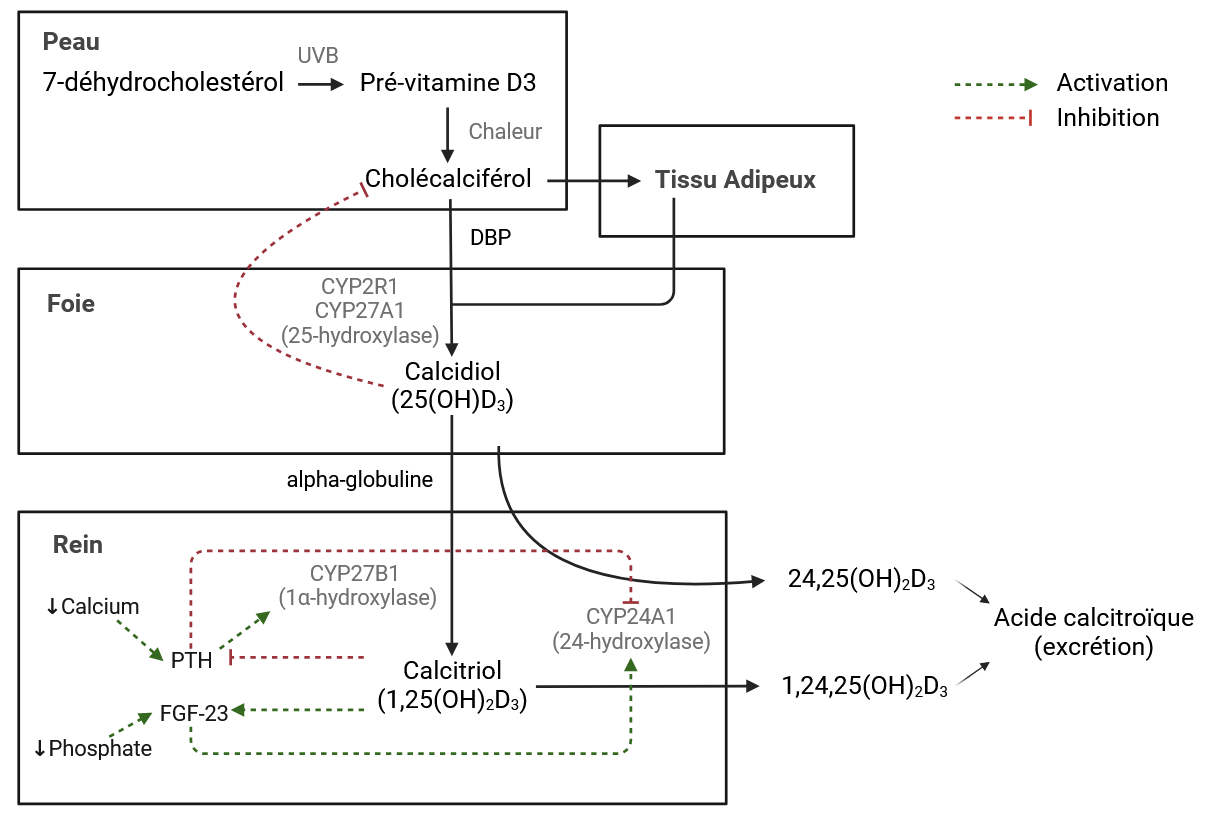
\includegraphics{figures/vitd-metabolism-fr.png}

}

\caption[Métabolisme de la vitamine
D.]{\label{fig-vitd-metabolism}\textbf{Métabolisme de la vitamine D.} Le
métabolisme de la vitamine D débute lorsque le 7-déhydrocholestérol,
présent dans la peau, est transformé par les rayons ultraviolets
provenant du soleil en cholécalciférol. Le cholécalciférol ou vitamine
D\textsubscript{3} est ensuite transporté par la protéine de liaison à
la vitamine D, et est métabolisé dans le foie par des enzymes
25-hydroxylases telles que le CYP2R1 en calcidiol ou \ac{25(OH)D3}.
L'autre étape du métabolisme se situe dans le rein, où après transport
du calcidiol, celui-ci se retrouve métabolisé en calcitriol ou
\ac{1,25(OH)2D3} par la \ac{CYP27B1}. \ac{DBP}, \acl{DBP}. La CYP24R1
est responsable du catabolisme de la vitamine D en métabolisant le
calcidiol et calcitriol en \ac{24,25(OH)2D3} et \ac{1,24,25(OH)3D3}
respectivement, où ils seront ensuite métabolisé par la même enzyme en
acide calcitroïque, qui sera excrété dans la bile du foie pour être
éliminé. D'après \textcite{Dankers.2017}, \textcite{Tsiaras.2011},
\textcite{Christakos.2010}, et \textcite{Prosser.2004}}

\end{figure}%

La synthèse du calcitriol est régulée par deux hormones, l'\acf{PTH} et
l'hormone de croissance des fibroblastes 23 (\acsu{FGF23}). La
\ac{FGF23}, induit par une concentration élevée de calcitriol et une
faible concentration de phosphate dans le sang, favorise l'induction de
la \ac{CYP24A1}, tandis que la \ac{PTH}, induite par une faible
concentration de calcium et inhibée par une forte concentration de
calcitriol, va induire la \ac{CYP27B1} et donc contribuer à la synthèse
du calcitriol \autocite{Dankers.2017,Christakos.2010}. La \ac{PTH} agit
également directement sur les os en augmentant la résorption osseuse et
augmentant ainsi la calcémie.

\section{Place de l'ergostérol}\label{place-de-lergostuxe9rol}

L'ergostérol ou vitamine D\textsubscript{2} est une autre forme de
vitamine D (\Cref{fig:ergo-struc}). Si les deux formes de vitamine sont
perçues comme interchangeables, la vitamine D\textsubscript{3} est
toutefois considérée plus intéressante en termes de traitement, car son
administration est plus efficace que celle de la vitamine
D\textsubscript{2} afin d'augmenter la concentration de calcidiol et
donc pour traiter les carences. En effet, la vitamine
D\textsubscript{2}, de nature végétale ou fongique, possède une
structure légèrement différente de la vitamine D\textsubscript{3}.

La métabolisation est fonctionnellement différente entre la vitamine
D\textsubscript{2} et vitamine D\textsubscript{3}. Ainsi, lors du
catabolisme de la vitamine D\textsubscript{2}, la 24-hydroxylation du
25(OH)D\textsubscript{2} et du
1,25(OH)\textsubscript{2}D\textsubscript{2} dans le rein conduit aux
métabolites 24,25(OH)\textsubscript{2}D\textsubscript{2} et
1,24,25(OH)\textsubscript{3}D\textsubscript{2} respectivement. Le
1,24,25(OH)\textsubscript{3}D\textsubscript{2} est inactif à la
différence de son analogue \ac{1,24,25(OH)3D3} qui nécessite une
oxydation supplémentaire afin d'être désactivée, et possède entre autres
une affinité pour le \ac{VDR} (jusqu'à 40 \% plus forte que
\ac{1,25(OH)2D3}). De plus, la 24-hydroxylation pourrait également avoir
lieu dans le foie, conduisant à la formation de
24(OH)D\textsubscript{2}. Le métabolite en résultant, la
1,24(OH)\textsubscript{2}D\textsubscript{2}, est moins affin pour le
\ac{VDR} comparé à son analogue D\textsubscript{3}. En revanche, la
vitamine D\textsubscript{3} ne subit pas cette première 24-hydroxylation
hépatique \autocite{Houghton.2006}. 1

\begin{figure}[ht]
\centering

\includegraphics[width=0.8\textwidth]{figures/ergo_vs_chole.png}
\caption[Comparaison de la structure de l'ergocalciférol par rapport au cholécalciférol.]{\textbf{Comparaison de la structure de l'ergocalciférol par rapport au cholécalciférol.} La structure de l'ergocalciférol comprend une double liaison et un groupement méthyl (CH\textsubscript{3}) supplémentaire par rapport au cholécalciférol. Cela implique une voie de métabolisation différente, notamment une voie d'élimination plus rapide, et donc une diminution de la concentration en métabolite biologiquement actif issue de l'ergocalciférol. \textcite{Houghton.2006}}
\label{fig:ergo-struc}

\vspace{1em}

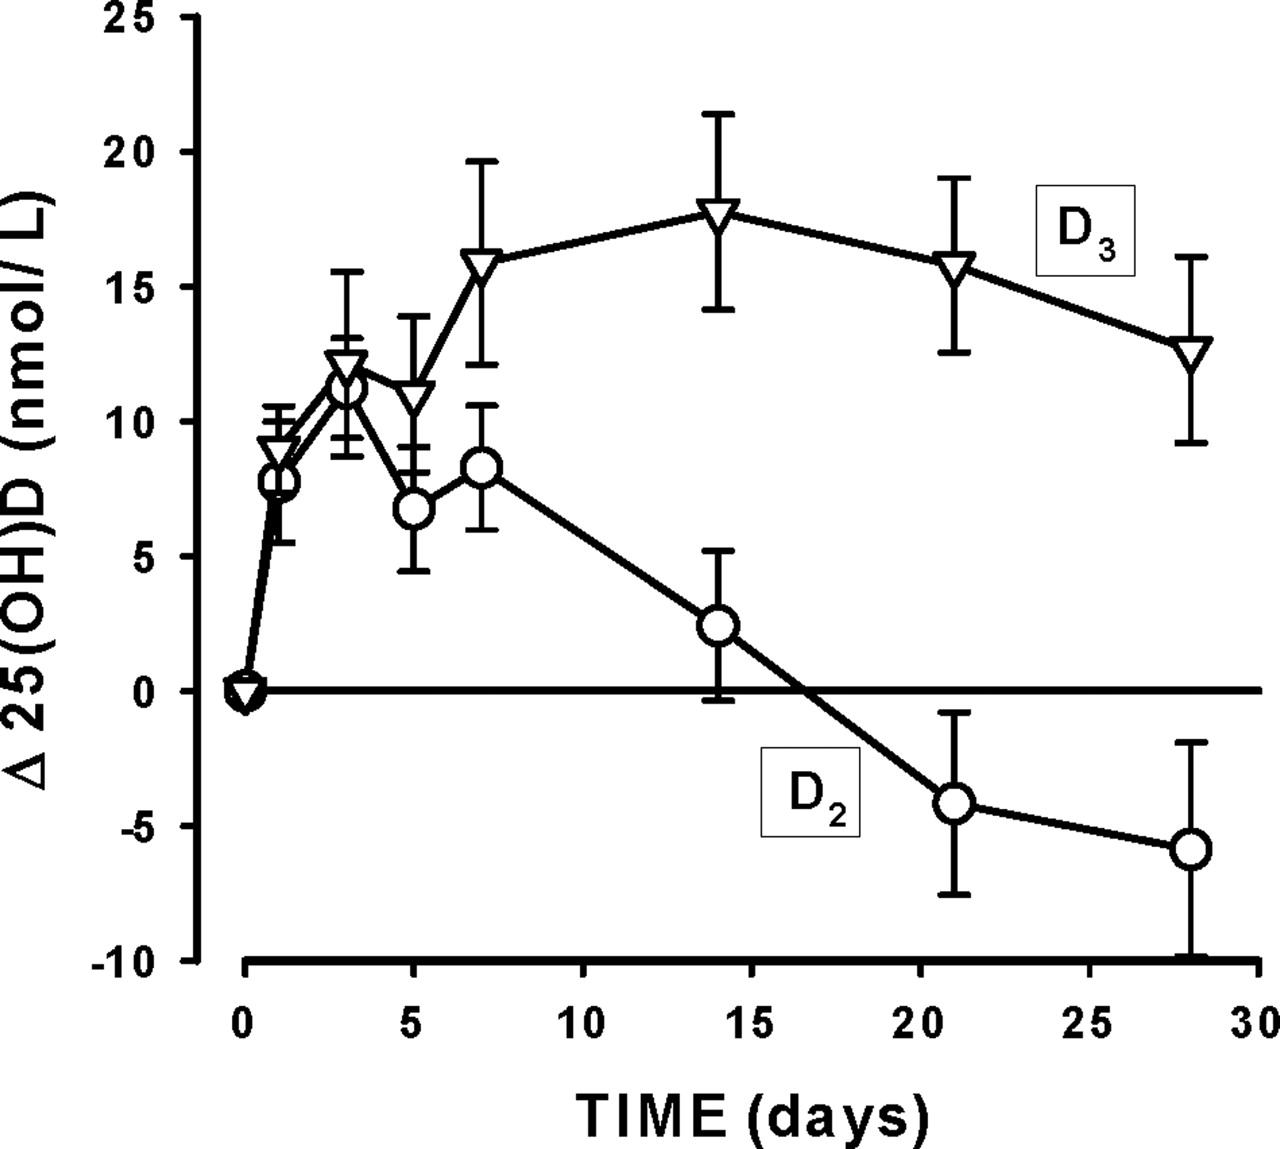
\includegraphics[width=0.8\textwidth]{figures/PK_D2_vs_D3.jpeg}
\caption[Evolution de la concentration en 25(OH)D après administration d'une dose de 50 000 UI de vitamine D\textsubscript{2} ou D\textsubscript{3} chez 10 patients.]{\textbf{Evolution de la concentration en 25(OH)D après administration d'une dose de 50 000 UI de vitamine D\textsubscript{2} ou D\textsubscript{3} chez 10 patients.} \textcite{Armas.2004}}
\label{fig:PK}
\end{figure}

De ce fait, la vitamine D\textsubscript{2} possède une pharmacocinétique
différente. La mesure de la capacité des deux formes de vitamine D à
maintenir les concentrations en \ac{25(OH)D} suite à l'administration
d'une dose de 50 000 UI des deux types de vitamine D (\Cref{fig:PK})
montre que la vitamine D\textsubscript{2} est inférieure à la vitamine
D\textsubscript{3}, malgré une phase d'absorption identique les trois
premiers jours, du fait d'une élimination beaucoup plus rapide
\autocite{Armas.2004}.

Selon les auteurs et la dose administrée, la vitamine D\textsubscript{3}
serait deux à trois fois plus efficace que la vitamine
D\textsubscript{2} pour augmenter la concentration en 25(OH)D
\autocites[ ]{Trang.1998}{Armas.2004}.

L'ergocalciférol continue d'être utilisée en tant que supplément aux
Etats-Unis \autocite{Houghton.2006}. Cependant, cette forme de
traitement reste moins efficace voire est insuffisante pour corriger les
déficits en vitamine D comparée au cholécalciférol, comme le montre
certains essais cliniques \autocite{Boyle.2005}.

Le cholécalciférol étant la forme de vitamine D possédant une meilleure
capacité à augmenter la concentration de calcidiol à long terme, il
devrait être privilégié lors de supplémentations. Pour ces raisons, nous
ne discuterons seulement que de la vitamine D\textsubscript{3} lorsque
nous examinerons l'usage et le potentiel thérapeutique de la vitamine D.

\section{Propriétés}\label{propriuxe9tuxe9s}

\subsection{Propriétés classiques
osseuses}\label{propriuxe9tuxe9s-classiques-osseuses}

L'usage de la vitamine D précède sa découverte avec l'utilisation de
l'huile de foie de morue décrite dans la littérature dès 1782 par Thomas
Percival, qui rapporte son usage et les effets bénéfiques constatés sur
le rhumatisme chronique en Angleterre 1782 par \autocite{Percival.1782}.
A cette époque, se multiplient chez l'enfant les cas de rachitisme, une
maladie caractérisée par le ramollissement et l'affaiblissement des os.
En France, Armand Trousseau compile en 1858 le Traité de thérapeutique
et de matière médicale, qui reprend les opinions contemporaines sur la
matière médicale et ses expériences, et décrit l'action thérapeutique de
l'usage de l'huile de foie de morue sur le rachitisme et fait
remarquablement disparaître tous les symptômes
\autocite{Trousseau.1858}. Il publie également son ouvrage Clinique
Médicale de l'Hôtel-Dieu en 1861, où il déclare que le rachitisme est
causé par une alimentation déséquilibrée que l'huile de foie de morue
peut résoudre \autocite{Hernigou.2019}. Le livre a été traduit en
anglais et est devenu célèbre \autocite{Hernigou.2019}.

Dans les années 1917--1922, les progrès concernant les causes et le
traitement du rachitisme se sont accélérées. \textcite{Hess.1917.lc}
démontrent que l'administration de l'huile de foie de morue permet de
prévenir et guérir du rachitisme chez les enfants afro-américains à New
York. En 1918, Mellanby a montré qu'il était possible de prévenir le
rachitisme expérimental chez des chiots avec de l'huile de foie de morue
et évoquait le rôle d'un ``facteur accessoire'' dans la production du
rachitisme \autocite{ORiordan.2014}. Par la suite, \textcite{Hess.1921}
ont rapporté que l'exposition au soleil permettait de guérir du
rachitisme. Ce sera \textcite{McCollum.1922} qui donnera le nom de
Vitamine D au ``facteur accessoire'' proposé par Mellanby
\autocite{Hernigou.2019,Mavrotas.2021}

L'intérêt pour la vitamine D s'est ensuite accru avec la découverte par
les scientifiques de son rôle crucial dans le métabolisme du calcium et
du phosphore. Depuis lors, de nombreuses études ont été menées pour
évaluer le rôle de la vitamine D dans le métabolisme osseux, et il est
désormais largement admis que la vitamine D joue un rôle essentiel dans
le maintien de la santé des os et des dents
\autocite{IOM.2011,Goltzman.2018}. Une carence en vitamine D est
associée à un risque accru d'ostéomalacie (une affection qui entraîne
une diminution de la masse osseuse) et d'ostéoporose (une affection
caractérisée par une fragilité des os).

L'action de la vitamine D est médiée par la liaison du calcitriol au
récepteur \ac{VDR}. En effet, le \ac{VDR} est un récepteur nucléaire
agissant comme un facteur de transcription. Le calcitriol rentre dans la
cellule cible et se lie au \ac{VDR}, induisant un changement
conformationnel et permettant de se lier à un autre récepteur \ac{RXR},
créant l'hétérodimère \ac{VDR}-\ac{RXR}. Ce complexe reconnaît une
séquence génétique spécifique appelée \ac{VDRE}, où l'hétérodimère
\ac{VDR}-\ac{RXR} et module ainsi l'expression des facteurs de
transcription \autocite{Dankers.2017,Pike.2010,Valdivielso.2009}.

La vitamine D agit directement sur le renouvellement osseux mais joue
également un rôle dans l'homéostasie du calcium. Cette dernière dépend
de l'absorption du calcium dans l'intestin, de sa réabsorption dans le
rein et de sa fixation/libération dans l'os. Le calcium est absorbé
grâce à des transporteurs transcellulaires (actifs) et par diffusion
paracellulaire (passive), sous le contrôle du calcitriol. Celui-ci est
considéré comme le principal facteur régulateur de l'absorption
intestinal de calcium. Lorsque les flux de calcium sont déséquilibrés,
les os servent de réservoir de calcium afin de maintenir l'équilibre
calcique. La réabsorption du calcium par le rein est contrôlée dans le
tubule contourné distal par l'action du calcitriol sur le \ac{VDR}
\autocite{Carmeliet.2015}. Ainsi, la vitamine D joue un rôle crucial
dans l'absorption intestinale du calcium et du phosphore, assurant ainsi
l'homéostasie du calcium et du phosphore dans l'organisme. Cependant, un
certain nombre des manifestations de la carence en vitamine D ne sont
pas totalement superposables à celles de l'invalidation du \ac{VDR}.

De plus, la liaison du calcitriol sur le VDR situé dans les ostéoblastes
entraîne une augmentation de la minéralisation osseuse et donc de la
fixation du calcium dans les os (diminution de RANKL, facteur de
transcription activant les ostéoclastes, et augmentation de LRP5)
\autocite{Carmeliet.2015}. Lorsque la calcémie est basse, l'augmentation
de la \ac{PTH} conduit à une augmentation de RANKL ce qui favorise la
résorption des os par les ostéoclastes afin d'augmenter la calcémie
(\Cref{fig-vitd-metabolism}).

\subsection{Propriétés
extra-osseuses}\label{propriuxe9tuxe9s-extra-osseuses}

La découverte des propriétés extra-osseuses de la vitamine D a commencé
avec le clonage du récepteur \ac{VDR} en 1987. Son identification dans
la majorité des tissus et populations cellulaires a ouvert la voie à de
nombreuses études fondamentales et cliniques autour du rôle pléiotrope
de la vitamine D \autocite{Rosen.2012}. Le \ac{VDR} est exprimé de façon
ubiquitaire ; cependant, certaines cellules ou tissus, tels que les
globules rouges, les muscles striés, et certaines cellules hautement
différenciés du cerveau telles que les cellules de Purkinje du cervelet,
n'expriment que faiblement \ac{VDR} \autocite{Bouillon.2008}.

Plus récemment l'intérêt pour la vitamine D a été étendu à différentes
pathologies diversement associées à des désordres osseux, en particulier
dans le cancer, les maladies cardio-métaboliques (obésité et diabète de
type 2, métabolisme du glucose) et les maladies auto-immunes (diabète de
type 1, sclérose en plaques, troubles thyroïdiens auto-immuns)
\autocite{Dankers.2017,Caprio.2017}. En effet, plusieurs recherchent
suggèrent que la vitamine D joue un rôle dans le diabète de type 2, en
stimulant l'expression des récepteurs à l'insuline et en augmentant la
sensibilité à l'insuline. Elle jouerait aussi un rôle dans l'obésité au
niveau du tissu adipeux, où des corrélations inverses ont été observées
entre le taux de calcidiol et la leptine (hormone régulant l'appétit) et
résistine (hormone pro-inflammatoire et contribue à la résistance à
l'insuline), et une association positive avec l'adiponectine (hormone
augmentant la sensibilité à l'insuline)
\autocite{Caprio.2017,Bellia.2013}. Il existe une association inverse
entre le taux de calcidiol et de marqueurs d'inflammation systémique
chez les sujets obèses \autocite{Bellia.2013}.

Un autre domaine d'intérêt concernant les effets extra-squelettiques de
la vitamine D concerne son rôle au niveau des muscles squelettiques.
Plusieurs études suggèrent que la vitamine D stimule la synthèse des
protéines musculaires ainsi que la réabsorption du calcium dans le
réticulum sarcoplasmique, ce qui permet de maintenir une force
musculaire adéquate \autocite{Caprio.2017}.

Enfin, la vitamine exercerait des effets régulateurs sur la fonction des
cellules immunitaires comme nous le verrons plus loin.

\begin{landscape}
\begin{figure}
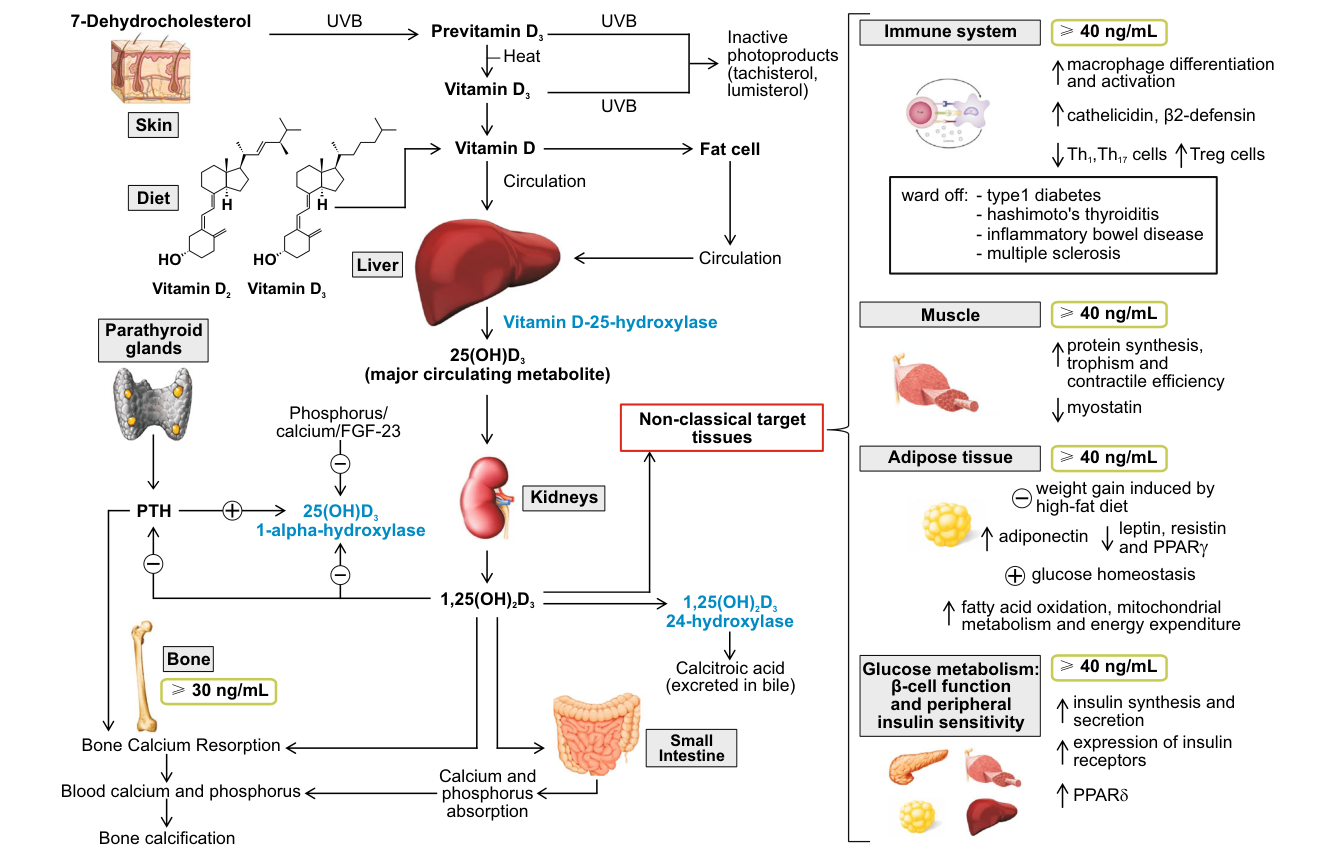
\includegraphics{figures/extra-skeletal-effect.png} 
\caption[Effets classiques et extra-squelettiques de la vitamine D.]
{\textbf{Effets classiques et extra-squelettiques de la vitamine D.} \textcite{Caprio.2017}}
\label{fig:extra-skeletal}
\end{figure}
\end{landscape}

La vitamine D exerce en plus de son action endocrine classique,
dépendante de la 1-hydroxylation par le rein, une action locale
autocrine et paracrine, par le biais d'une expression locale de
l'hydroxylase \ac{CYP27B1} dans différents tissus
\autocite{Carmeliet.2015,Cannell.2008}. Cela concerne notamment l'action
de la vitamine D sur l'immunité.

Cependant, selon certains auteurs, les bénéfices extra-squelettiques de
la vitamine D ne seraient notables que lorsque la concentration de
calcidiol serait supérieure au seuil de 20-30 ng/mL actuellement
recommandé par les autorités de santé. Les données contradictoires des
études cliniques randomisées sur les effets de la supplémentation en
vitamine D ne permettent pas de trancher \autocites[ ]{Caprio.2017}[
]{Lewis.2015}{Bouillon.2013,Rejnmark.2017}.

\section{Dose thérapeutique
efficace}\label{dose-thuxe9rapeutique-efficace}

\subsection{Unités}\label{unituxe9s}

L'expression de la dose de la vitamine D peut se faire en plusieurs
unités. Classiquement, c'est l'\ac{UI} qui est utilisée. Elle peut
également être exprimée en masse lors de prises de comprimés.
L'équivalence est de 1 µg pour 40 \ac{UI} ou 1 \ac{UI} pour 0,025 g. La
concentration de vitamine D (en fait celle de calcidiol utilisée comme
marqueur du statut vitaminique) est définie en ng/mL ou en nmol/L. Pour
passer de ng/mL en nmol/L, il suffit de multiplier par 2.5
\autocite{Pramyothin.2012}

Cependant la \ac{FDA} a décidé depuis janvier 2021 de passer à une dose
écrite en microgramme, ce qui oblige les fabricants à donner
l'information en microgramme, bien que la dénomination en UI reste
possible en parallèle \autocite{HHS.2016}.

Un essai-clinique visant à établir l'efficacité de la supplémentation en
cholécalciférol a été réalisée chez 61 patients, selon trois schémas
d'administration : 1000 UI par jour, 7000 UI par semaine ou 30 000 UI
par mois. Les patients inclus étaient carencés en début d'étude avec une
concentration de calcidiol inférieure à 20 ng/mL (en moyenne autour de
13,3 ng/mL) et ont été suivi pendant 3 mois. L'étude a permis de
déterminer que, en moyenne, une supplémentation en cholécalciférol
augmente la concentration de calcidiol de 1.3 ng/100 UI par jour
\autocite{Takács.2017}.

\subsection{Dose recommandée
journalière}\label{dose-recommanduxe9e-journaliuxe8re}

Actuellement, l'Académie américaine de médecine (anciennement Institute
of Medicine, \acsu{IOM}) est responsable des recommandations émises par
la \ac{FDA}, l'équivalent de l'\ac{ANSM} en France. L'\ac{AJR} pour la
vitamine D est de 600 UI par jour tous sexes confondus de 1 à 70 ans, et
reste le même en cas de grossesse ou d'allaitement \autocite{IOM.2011}.
L'\ac{AJR} est augmentée à 800 UI/jour chez les personnes de plus de 70
ans en raison de la plus grande variabilité des données disponibles
concernant cette catégorie d'âge. Une concentration sanguine de
calcidiol de 20 ng/mL ou plus est considérée par l'\ac{IOM} comme étant
le minimum adéquat chez 97,5 \% des personnes en bonne santé. Cette
concentration minimum de 20 ng/mL a été observé comme étant associée
pour la majorité de la population générale à une bonne santé osseuse
définie en termes de densité minérale osseuse et d'absorption du
calcium, d'accrétion et de maintenance osseuse, et de diminution du
risque d'ostéomalacie ou de rachitisme. Les concentrations de calcidiol
supérieures à 30 ng/mL ne sont pas associées à un bénéfice
supplémentaire selon l'\ac{IOM} \autocite{IOM.2011,Rosen.IOM.2012}.

Un autre acteur français, l'\ac{ANSES}, stipule que les recommandations
journalières de cholécalciférol sont de 15 µg par jour pour un adulte,
soit l'équivalent d'une dose de 600 UI/j, s'appuyant sur les
recommandations de l'Autorité européenne de sécurité des aliments
(\acsu{EFSA}) \autocite{ANSES.2021}. En effet, l'\ac{EFSA} a retenu une
valeur de 15 µg/j (soit 600 UI/j) permettant aux hommes et femmes
d'atteindre le seuil de calcidiol jugé adéquat de 50 nmol/L ou 20 ng/mL
\autocite{ANSES.2022.note} (\Cref{tbl-seuil}).

\begin{table}
\caption[Tableau comparatif des seuils d'adéquation de la vitamine D par différentes sources.]{\textbf{Tableau comparatif des seuils d'adéquation de la vitamine D par différentes sources.} IOM : Institut de Médecine ; ANSES : Agence nationale de sécurité sanitaire de l’alimentation, de l’environnement et du travail. D'après \textcite{IOM.2011} et \textcite{ANSES.2021}}
\label{tbl-seuil}
\centering
\begin{tabular}{ccc}
\toprule
\textbf{Seuil de vitamine D} & \textbf{IOM} & \textbf{ANSES}\\
\midrule
Déficience en vitamine D & < 12 ng/mL & < 10 ng/mL\\
Insuffisance en vitamine D & 12-20 ng/mL & 10-20 ng/mL\\
Valeurs recommandées & 20-30 ng/mL & 20-30 ng/mL\\
Limite Supérieure de Sécurité & > 50 ng/mL  & > 100 ng/mL \\
\bottomrule
\end{tabular}
\end{table}

\begin{table}
\centering
\caption[Apports journaliers recommandés de la vitamine D (UI/j)]{\textbf{Apports journaliers recommandés de la vitamine D (UI/j).} La mention d'\ac{AJR} indique que l'apport couvre les besoins minimum de 97,5 \% de la population pour atteindre une concentration de 20 ng/mL selon l'\ac{IOM}. D'après \textcite{ANSES.2021, IOM.2011}}
\label{tbl-AJR}
\begin{tabular}{ccc}
\toprule
\textbf{Groupe d'âge} & \textbf{IOM} & \textbf{ANSES/EFSA} \\
\midrule
Nourrissons (0-12 mois) & 400 & 400 \\
Enfants (1 - 11 ans) & 600 & 600 \\
Adolescents (11 - 17 ans) & 600 & 600 \\
Hommes et Femmes & 800 & 600 \\
Femmes enceintes & 600 & 600 \\
\bottomrule
\end{tabular}
\end{table}

\subsection{Controverse autour de la dose recommandée
journalière}\label{controverse-autour-de-la-dose-recommanduxe9e-journaliuxe8re}

Plusieurs acteurs tels que la Société d'Endocrinologie suggèrent que les
\ac{AJR} établis par l'\ac{IOM} sont insuffisants. La Société
d'Endocrinologie suggère un \ac{AJR} de 1500 UI/j pouvant aller à 2000
UI/j pour des adultes, avec des recommandations ciblées pour des
populations à risque avec des maladies spécifiques pour lesquelles le
seuil minimal de calcidiol serait de 30 ng/mL. L'\ac{IOM} suggère dans
une réponse à la Société d'Endocrinologie que les auteurs ont fait un
amalgame entre apports nutritionnels pour la population générale et
l'établissement des recommandations pour des personnes à risque, ce qui
inclut des conditions adéquates pour la population générale
\autocite{Rosen.IOM.2012}. De plus, l'\ac{IOM} est en désaccord en qui
concerne les bénéfices osseux, concluant sur la base de la littérature
qu'il n'y a pas de bénéfices osseux observés au-delà de 20 ng/mL, qui
est le seuil permettant de couvrir les besoins minimes de 97,5 \% de la
population (\Cref{tbl-seuil}). L'\ac{IOM} conclut que les bénéfices
extra-squelettiques de la vitamine D sont incertains et que les preuves
ne sont pas suffisantes pour recommander une augmentation de l'\ac{AJR}
\autocite{IOM.2011}.

\section{Utilisation thérapeutique}\label{utilisation-thuxe9rapeutique}

La vitamine D est surtout utilisée en thérapeutique afin de prévenir les
carences à des fins de bonne santé osseuse. Elle permet de prévenir le
rachitisme chez les enfants et l'ostéoporose chez les adultes et surtout
chez les personnes âgées. Elle permet de maintenir une bonne densité
osseuse et une absorption du calcium adéquat et prévient du rachitisme
et de l'ostéomalacie.

La vitamine D possède également un potentiel thérapeutique dans le
traitement des maladies auto-immunes. De ce fait, le groupe clinique
dirigé par Cicero Coimbra au Brésil utilise de fortes doses quotidiennes
de vitamine D, allant de 40 000 UI à 300 000 UI, pour traiter la
sclérose en plaques et le vitiligo. Le statut clinique des patients
atteints de psoriasis et le degré de repigmentation chez les patients
atteints de vitiligo s'améliorent de manière significative
\autocite{Amon.2022}. Néanmoins, il s'agit d'une circonstance
particulière où cette approche repose sur l'hypothèse que ces maladies
auto-immunes sont dues à une résistance à la vitamine D
\autocite{Lemke.2021}.

\section{Pharmacocinétique}\label{pharmacocinuxe9tique}

La pharmacocinétique de la vitamine D est beaucoup plus complexe que
celle d'un agent pharmacologique standard, en raison de l'hydroxylation
progressive nécessaire pour obtenir sa forme active, et de la présence
de ses métabolites dans la circulation et les tissus. De plus, sa
liaison à son transporteur \acsu{DBP} influence les propriétés des
métabolites de la vitamine D \autocite{Schoenmakers.2018}. Comme nous
l'avons vu (\textbf{Section~\ref{sec-metabolisme}}), la vitamine D est
hydroxylée en calcidiol par le CYP2R1, une enzyme possédant une haute
capacité de métabolisation : la demi-vie de la vitamine D non hydroxylée
est donc faible et il est possible d'observer le cholécalciférol en
concentration substantielle dans le plasma lors que la dose sature la
capacité de l'enzyme \autocite{Schoenmakers.2018}.

\begin{figure}

\centering{

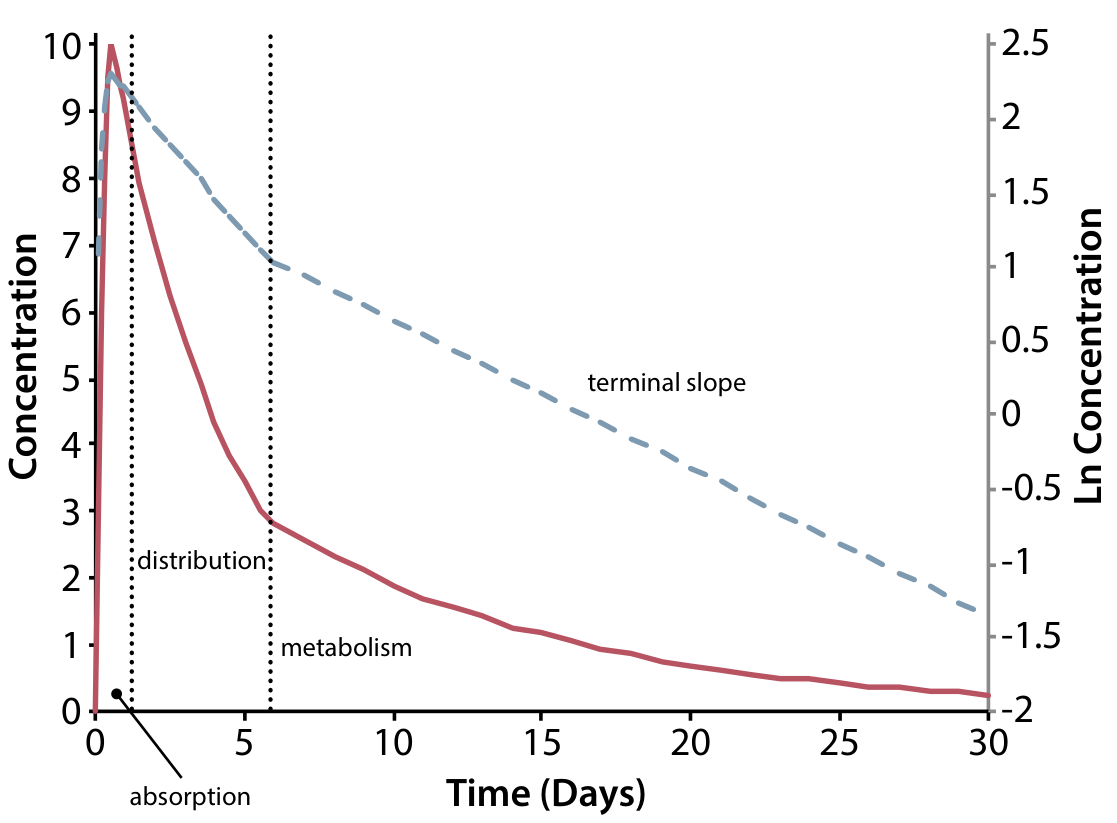
\includegraphics{figures/Schoenmakers.2018 - Plasma appearance and disappearance of 25(OH)D after oral intake.png}

}

\caption[Schéma des phases pharmacocinétiques du
cholécalciférol]{\label{fig-PK-all-VitD}\textbf{Schéma des phases
pharmacocinétiques du} \ac{25(OH)D3}. La ligne pointillée correspond au
logarithme naturel de la concentration duquel les différentes pentes et
les demi-vies sont calculées. \autocite{Schoenmakers.2018}}

\end{figure}%

\subsection{Absorption}\label{absorption}

La vitamine D (en tant que cholécalciférol) possède une absorption
rapide et linéaire, atteignant la \ac{Cmax} pour une dose de vitamine
D\textsubscript{3} à un \ac{Tmax} de 6 à 10 heures. Le calcidiol est
absorbé plus rapidement que le cholécalciférol, avec un \ac{Tmax} de 4 à
6 heures (\Cref{fig-PK-all-VitD}) \autocite{Schoenmakers.2018}.

Le cholécalciférol absorbé dans le tractus digestif, suit la même voie
d'absorption que les autres substances liposolubles. Le cholécalciférol
passe par les entérocytes où il se retrouve associée aux chylomicrons.
Elle peut puis est redistribuée entre les lipoprotéines, et enfin est
transférée vers la protéine de transport principale, la \ac{DBP}
(\Cref{fig-vd-absorption}). Le cholécalciférol associé au chylomicron
peut être transféré à la \ac{DBP} ou passer dans la circulation
sanguine.

Le calcidiol quant à lui est absorbé en majeure partie par la veine
porte du foie en diffusant à travers l'entérocyte et en mineure partie
absorbée par les chylomicrons. La majorité des métabolites de la
vitamine D, dont le calcidiol, est lié à la \ac{DBP}( à environ (85 \%),
et plus faiblement à l'albumine (15 \%) \autocite{Bikle.2017}.

\begin{figure}

\centering{

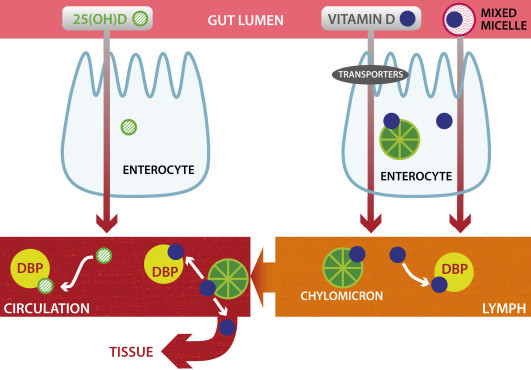
\includegraphics{figures/Schoenmakers.2018-vd-absorption.jpg}

}

\caption[Schéma de l'absorption de la vitamine D et du
calcidiol.]{\label{fig-vd-absorption}\textbf{Schéma de l'absorption de
la vitamine D et du calcidiol} \autocite{Schoenmakers.2018}. Le
cholécalciférol passe par des transporteurs actifs dans les entérocytes
où il se retrouve associé aux chylomicrons. Après être relâché dans la
lymphe, le cholécalciférol peut être transféré au \ac{DBP} ou suivre le
métabolisme du chylomicron qui peut relâcher le cholécalciférol dans les
tissus. Le calcidiol diffuse à travers l'entérocyte où il est lié en
grande majorité au \ac{DBP} plasmatique. \ac{DBP}, \acl{DBP}}

\end{figure}%

\subsection{Distribution}\label{distribution}

La vitamine D étant une molécule liposoluble, elle est principalement
distribuée dans les tissus adipeux où elle sert de compartiment de
stockage, mais également les tissus musculaires. Elle peut se retrouver
dans divers autres tissus tels que la peau, le plasma et d'autres
organes. Dans les réserves adipeuses vitamine D peut varier
considérablement entre 10 à 900 nmol/kg et il a été mesuré dans une
étude que le calcidiol pouvait varier de 2,3 à 12,8 nmol/kg. Une
corrélation positive existe entre la concentration de cholécalciférol
plasmatique et adipeuse mais elle n'est pas constamment retrouvée pour
le calcidiol.

Il n'existe pas encore d'études concernant la concentration de la
vitamine D dans les muscles chez les humains, mais des études conduites
sur des porcs nous permettent de faire des observations et
approximations. Ainsi, les muscles détiennent autour de 10\%--20\% du
cholécalciférol distribuée dans les tissus adipeux. Le ratio du
calcidiol entre le tissu adipeux et le muscle est plus élevé, variant
entre 0.5 à 1 en fonction de l'alimentation et du type de fibre
musculaire (rouge ou blanche). La concentration de calcidiol varie entre
75\% et 150\% du cholécalciférol présent dans les tissus adipeux
\autocite{Schoenmakers.2018}. La vitamine D étant une molécule
liposoluble et se distribuant abondamment dans les tissus adipeux, il
est possible de considérer que ce compartiment de distribution ait un
impact sur la pharmacocinétique de la vitamine D; le tissu adipeux
fonctionnerait comme un lieu de stockage et libèrerait de la vitamine D
sur le long terme dans la circulation sanguine.

Des données récentes suggèrent que la perte de poids n'influence pas le
statut en vitamine D. De plus, il n'est pas certain que la mobilisation
de la vitamine D et du calcidiol repose sur la diffusion de la forme
libre ou liée, ou qu'elle soit régulée, et l'impact de la masse adipeuse
sur la pharmacocinétique de la vitamine D est encore méconnu
\autocite{Schoenmakers.2018}.

Cependant il est connu que la dose nécessaire de vitamine D à
administrer pour atteindre le seuil thérapeutique doit augmenter lorsque
la masse graisse augmente, puisqu'un des compartiments de distribution
est plus grand, représenté par la masse graisseuse. La relation entre
l'\ac{IMC} a été étudiée par \textcite{Ekwaru.2014}. Ekwaru montre ainsi
la relation dose-réponse entre l'administration orale de cholécalciférol
et la concentration plasmatique de calcidiol pour l'ensemble des
individus (\Cref{subfig:vd-dose-response}), puis lorsque les sujets sont
classés selon leur \ac{IMC} (\Cref{subfig:vd-dose-imc}). Les auteurs
observent une relation dose-réponse exponentielle, où l'augmentation de
la concentration sérique de calcidiol diminue avec l'augmentation des
niveaux de supplémentation orale en vitamine D. Ils observent également
que les sujets ayant un \ac{IMC} plus élevé ont besoin d'une dose plus
élevée de vitamine D pour atteindre le même niveau de concentration
plasmatique de calcidiol.

\begin{figure}[H]
    \centering
    \begin{subfigure}{0.48\textwidth}
        \centering
        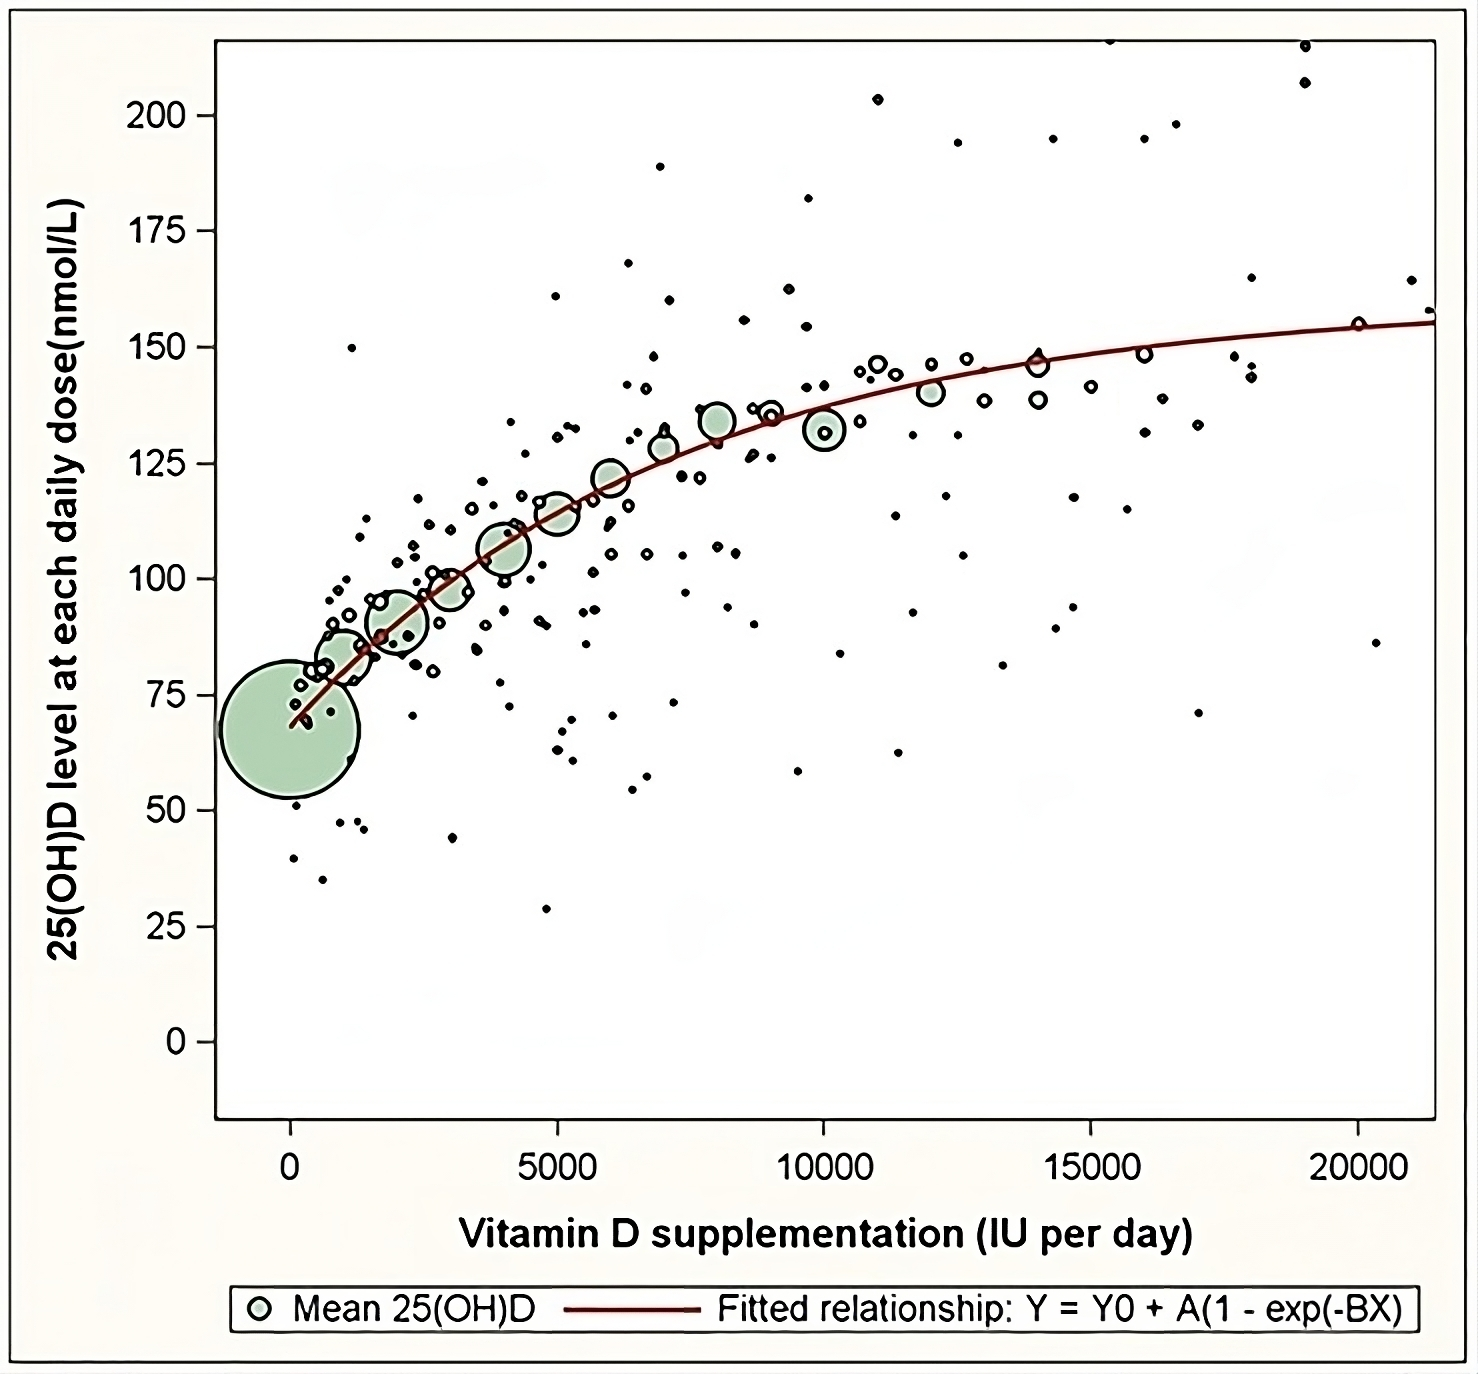
\includegraphics[width=\textwidth]{figures/ekwaru-dose-relation-transformed.jpg}
        \subcaption{Courbe dose-réponse de la supplémentation orale en vitamine D \ac{25(OH)D3} \autocite{Ekwaru.2014}.}
        \label{subfig:vd-dose-response}
    \end{subfigure}
    \hfill
    \begin{subfigure}{0.48\textwidth}
        \centering
        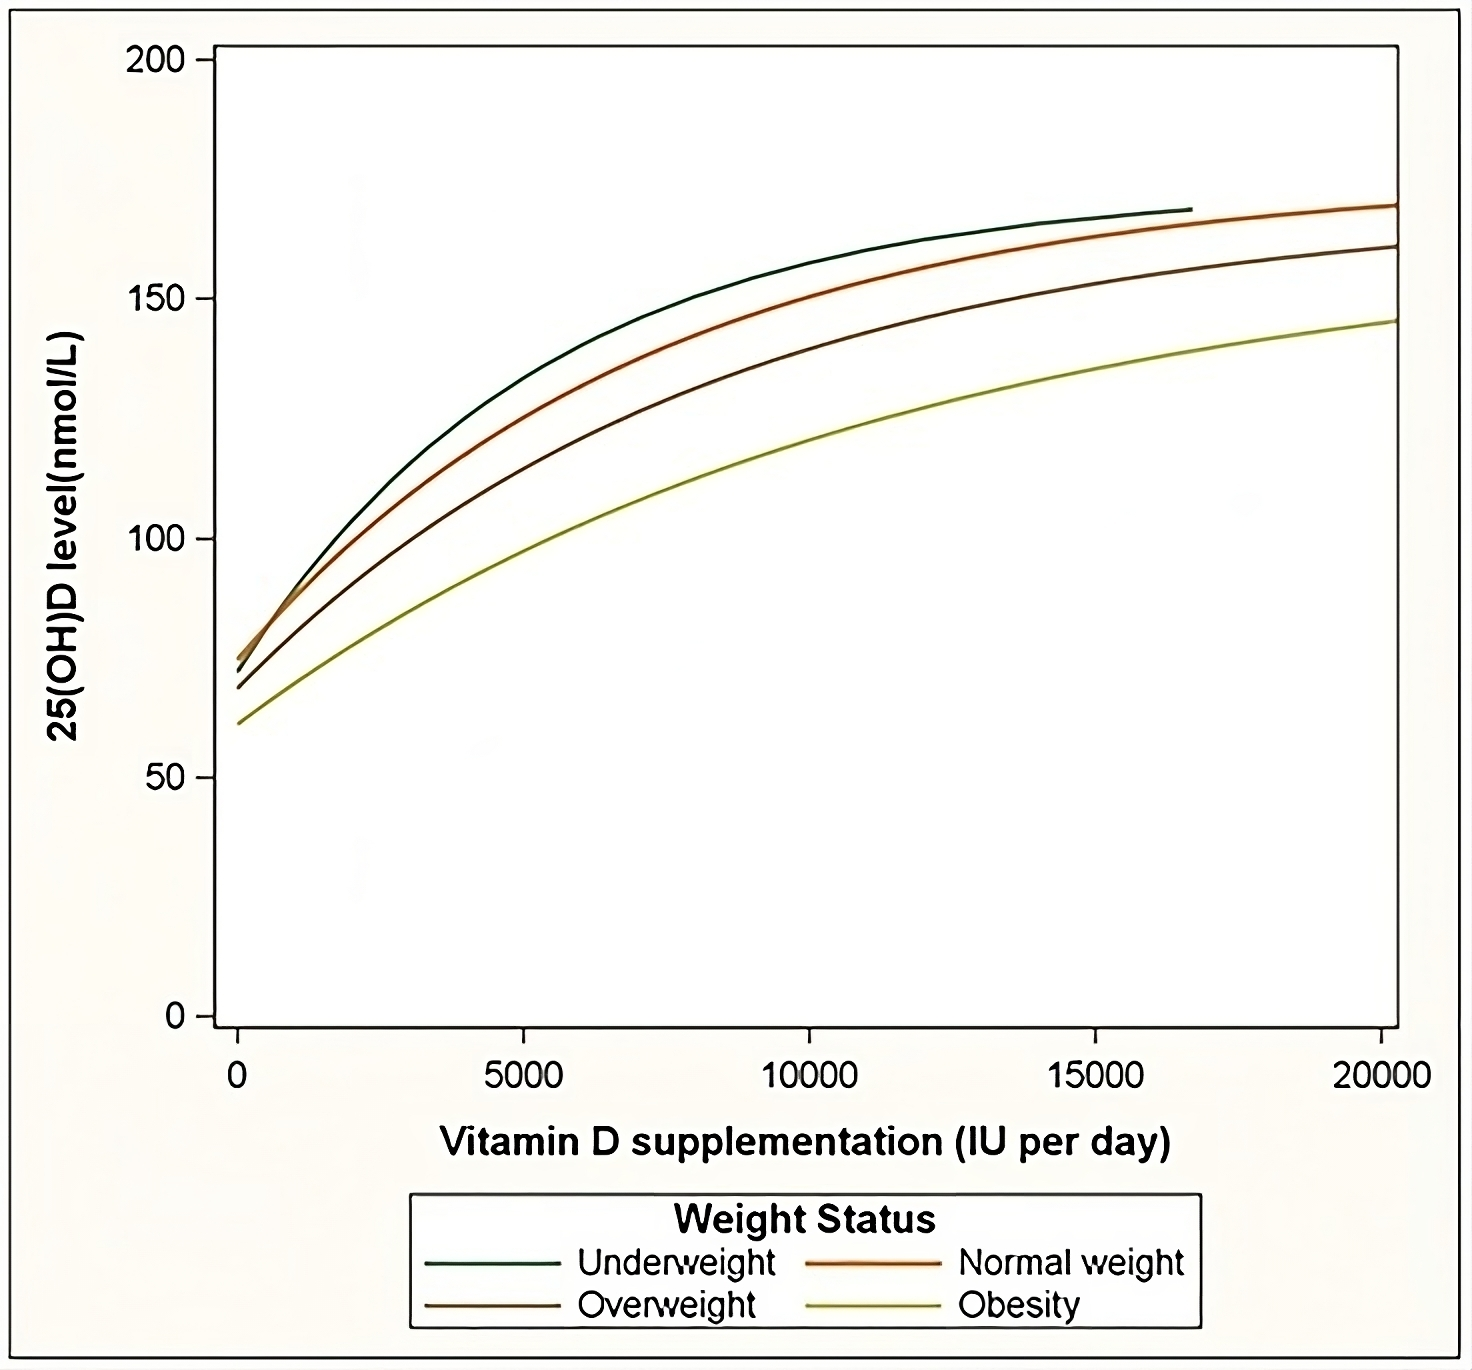
\includegraphics[width=\textwidth]{figures/ekwaru-dose-imc-transformed.jpg}
        \subcaption{Comparaison des courbes dose-réponse en fonction de l’indice de masse corporelle \autocite{Ekwaru.2014}.}
        \label{subfig:vd-dose-imc}
    \end{subfigure}
    \caption[Courbes dose-réponse de la supplémentation en vitamine D orale.]{\textbf{Courbes dose-réponse de la supplémentation en vitamine D orale.}}
    \label{fig:dose-response}
\end{figure}

Les auteurs notent que l'\ac{IMC} est un meilleur indicateur que le
poids absolu afin de juger de la quantité de vitamine D à administrer.
L'\ac{IOM} confirme également cette relation non linéaire avec une
augmentation plus marquée des concentrations sériques de calcidiol à des
doses inférieures à 1000 UI/j. La réponse est plus aplatie lorsque les
doses sont supérieures à 1000 UI/j \autocite{IOM.2011,Garland.2011}. De
ce fait, l'augmentation en vitamine D obtenue par supplémentation est
moindre lorsque la concentration initiale de vitamine D est plus élevée
(\Cref{fig:vd-expected-rise}).

\begin{figure}[H]
\centering
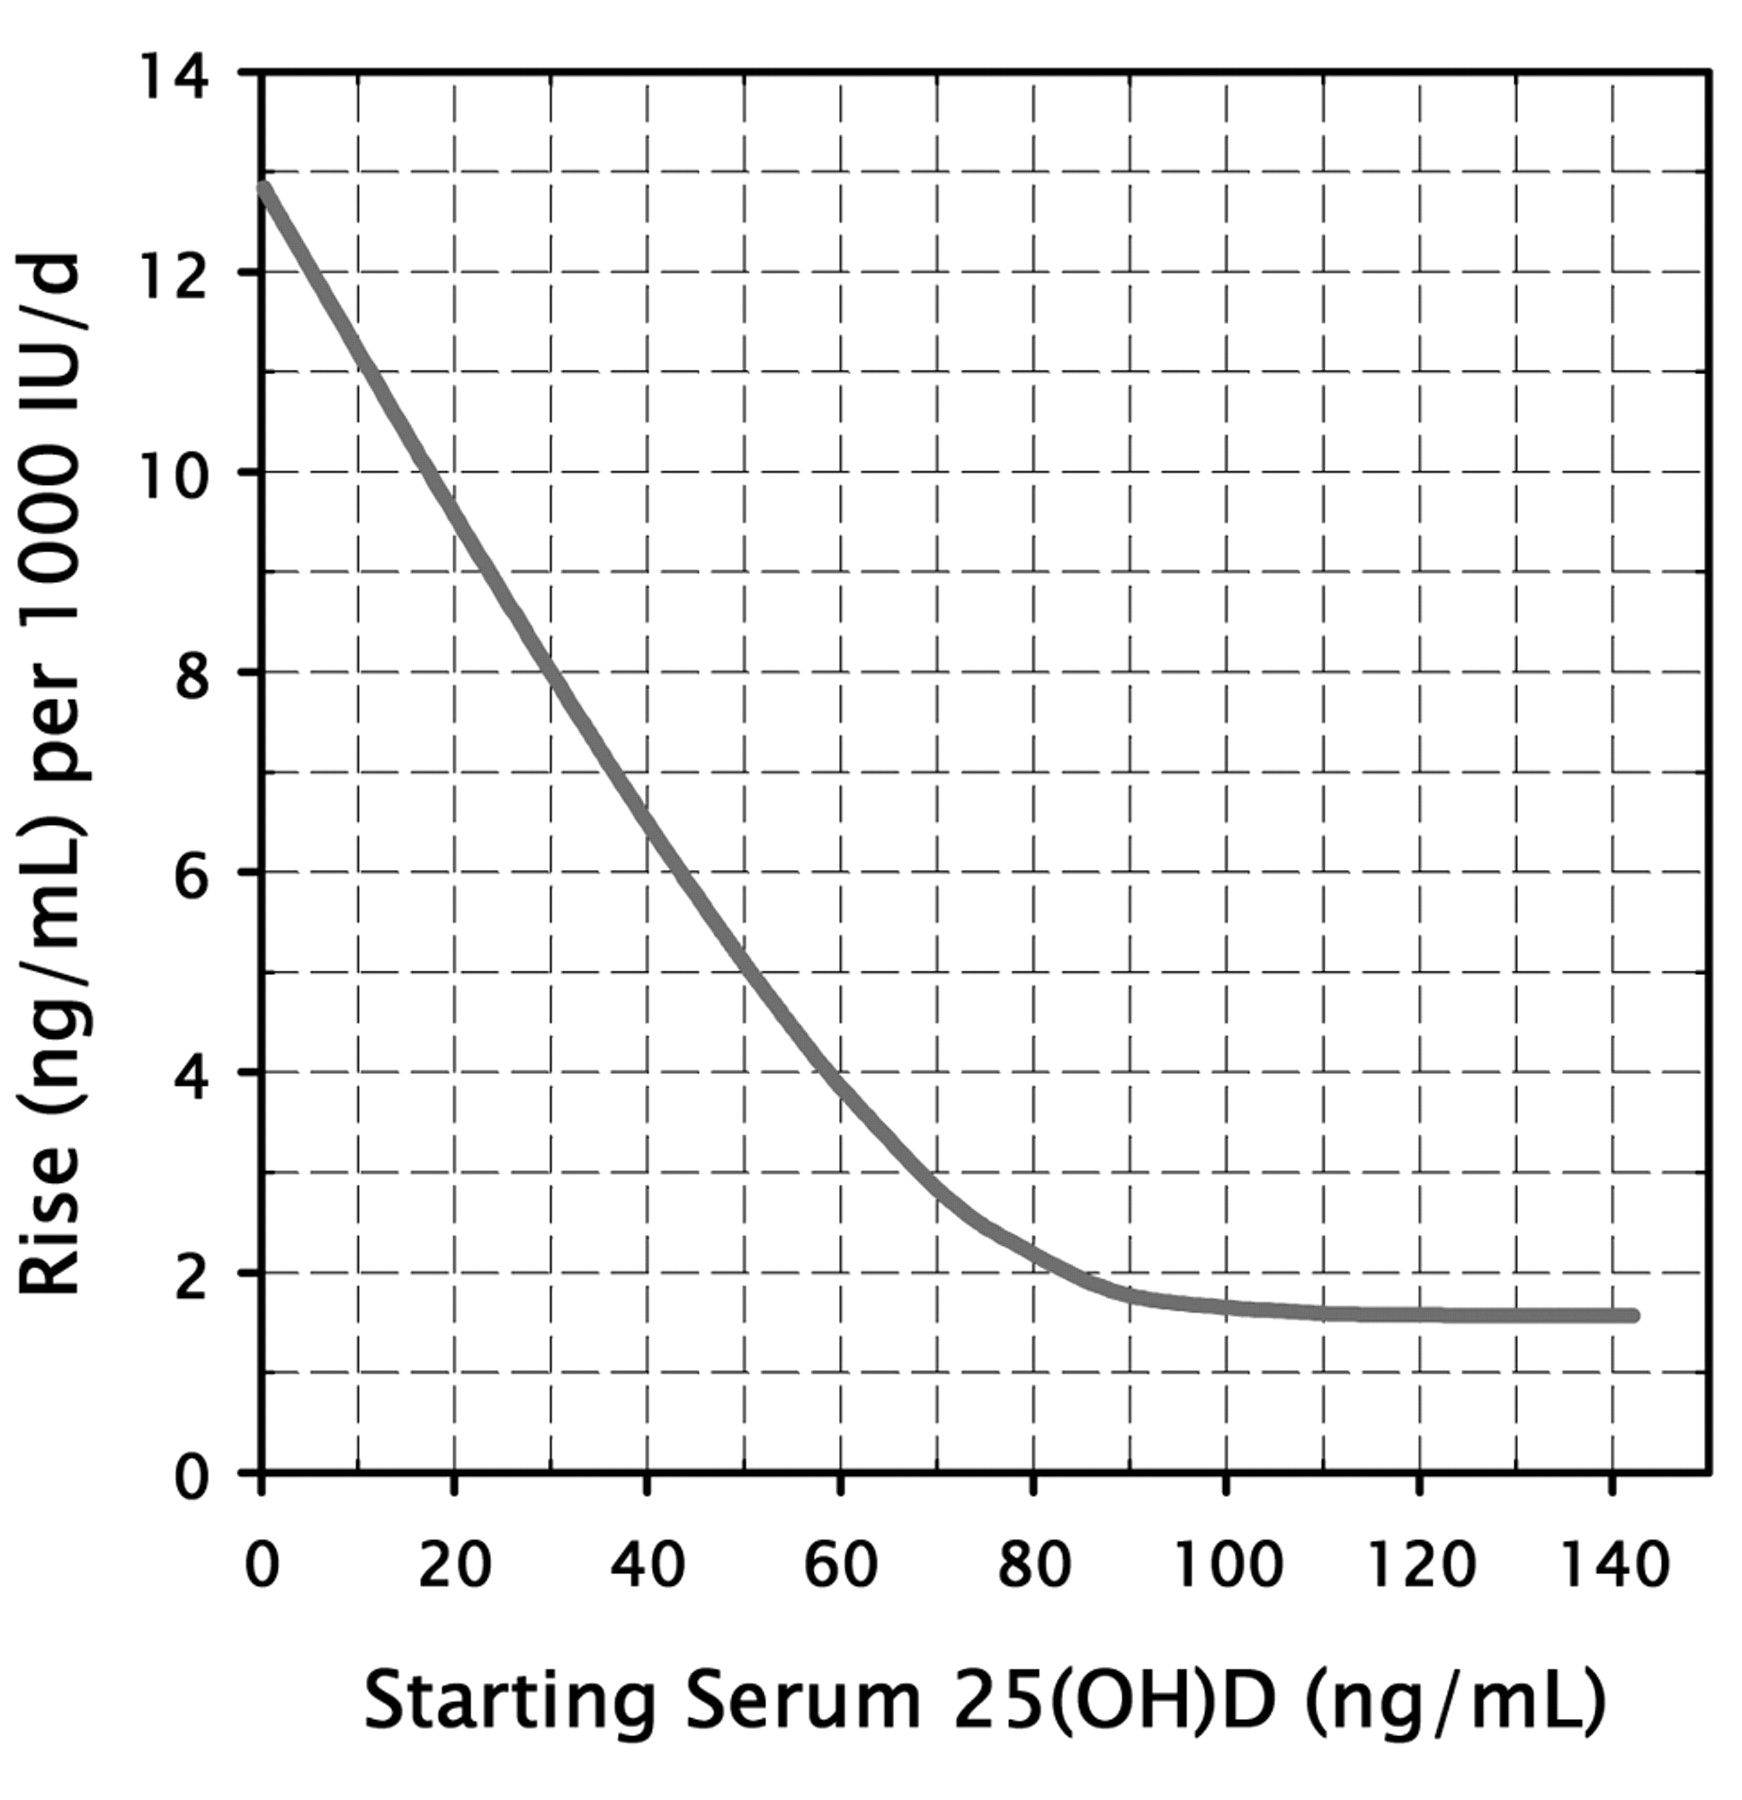
\includegraphics[width=0.5\textwidth]{figures/vd-expected-rise.jpeg}
\caption[Courbe de l'augmentation attendue de la 25(OH)D sérique pour chaque supplément de 1,000 UI de vitamine D3 par jour, en fonction de la valeur de base de la 25(OH)D de base]{\textbf{Courbe de l'augmentation attendue de la 25(OH)D sérique pour chaque supplément de 1,000 UI de vitamine D3 par jour, en fonction de la valeur de base de la 25(OH)D de base.} \autocite{Garland.2011}.}
\label{fig:vd-expected-rise}
\end{figure}

\subsection{Catabolisme et demi-vie}\label{catabolisme-et-demi-vie}

Le catabolisme de la vitamine D passe principalement par le \ac{CYP24A1}
et est exprimé universellement dans les cellules contenant le \ac{VDR}
régulant ainsi la stimulation du calcitriol sur l'expression des gènes
par son catabolisme. Elle est induite lorsque la concentration de
vitamine D devient élevée (\textgreater{} 220 nM ou 88 ng/mL). Elle
convertit ainsi le calcidiol et le calcitriol en métabolites
intermédiaires qui seront ensuite converti en acide calcitroïque par la
\ac{CYP24A1} où il sera éliminé par excrétion biliaire
\autocite{Schoenmakers.2018,Prosser.2004}.

La demi-vie du cholécalciférol est de 24 heures, et celle du calcidiol
de 10 à 40 jours, tandis que, comparativement, le calcitriol possède une
demi-vie très courte de 5 à 80 heures. Le métabolite \ac{24,25(OH)2D3}
possède quant à lui une demi-vie de 7-16 jours
\autocite{Schoenmakers.2018}. On observe ainsi que la vitamine D est
absorbée très rapidement, et se distribue rapidement dans les tissus,
mais que sa demi-vie est très longue, maintenant une concentration
plasmatique stable pendant plusieurs semaines (\Cref{fig-PK-all-VitD}).

\section{Toxicité}\label{toxicituxe9}

A dose toxique, la vitamine D induit un état hypercalcémique et
hypercalciurique, ce qui suggère un excès d'activité lié aux effets du
calcitriol \autocite{Vieth.1990}. Cet état s'accompagne d'une
suppression de l'activité de la \ac{PTH}, en raison de l'état
hypercalcémique qui exerce un rétrocontrôle négatif sur la \ac{PTH}
\autocites[ ]{Marcinowska-Suchowierska.2018}{Dusso.2005}. L'apport
excessif de cholécalciférol serait corrélée à une augmentation de
calcidiol qui induirait une augmentation de l'absorption intestinale du
calcium et de la résorption osseuse \autocite{Jones.2008,IOM.2011}.
Selon \textcite{Shepard.1980}, l'hypercalcémie proviendrait probablement
plus de cette résorption osseuse plutôt que de l'absorption intestinale
accrue du calcium

La symptomatologie de cette toxicité résulte principalement de
l'hypercalcémie et de l'hyperphosphatémie \autocites[
]{DeLuca.2011}{Janoušek.2022,Jones.2008,IOM.2011} affectant divers
organes. Les manifestations cliniques concernent notamment des troubles
gastro-intestinaux, des troubles du système cardiovasculaire ainsi que
des troubles du système musculo-squelettique. Le système rénal est
également impacté, et un trouble neurologique est également possible
(\Cref{fig-hypervitaminose-d}) \autocites[
]{Alshahrani.2013}{Janoušek.2022}. L'hypercalcémie peut également
conduire à une calcification des tissus mous, et des vaisseaux sanguins.
L'ensemble de ces conséquences cardiovasculaires et rénales causant une
défaillance de ces systèmes est probablement à l'origine de la mortalité
par intoxication à la vitamine D. L'ensemble de ces conséquences
cardiovasculaires et rénales causant une défaillance de ces systèmes est
probablement à l'origine de la mortalité par intoxication à la vitamine
D. Il est intéressant de noter que l'hypothèse selon laquelle un apport
excessif en vitamine D pourrait être associé à la formation de calculs
rénaux n'est pas appuyée par les données disponibles \autocite{IOM.2011}

\begin{figure}

\centering{

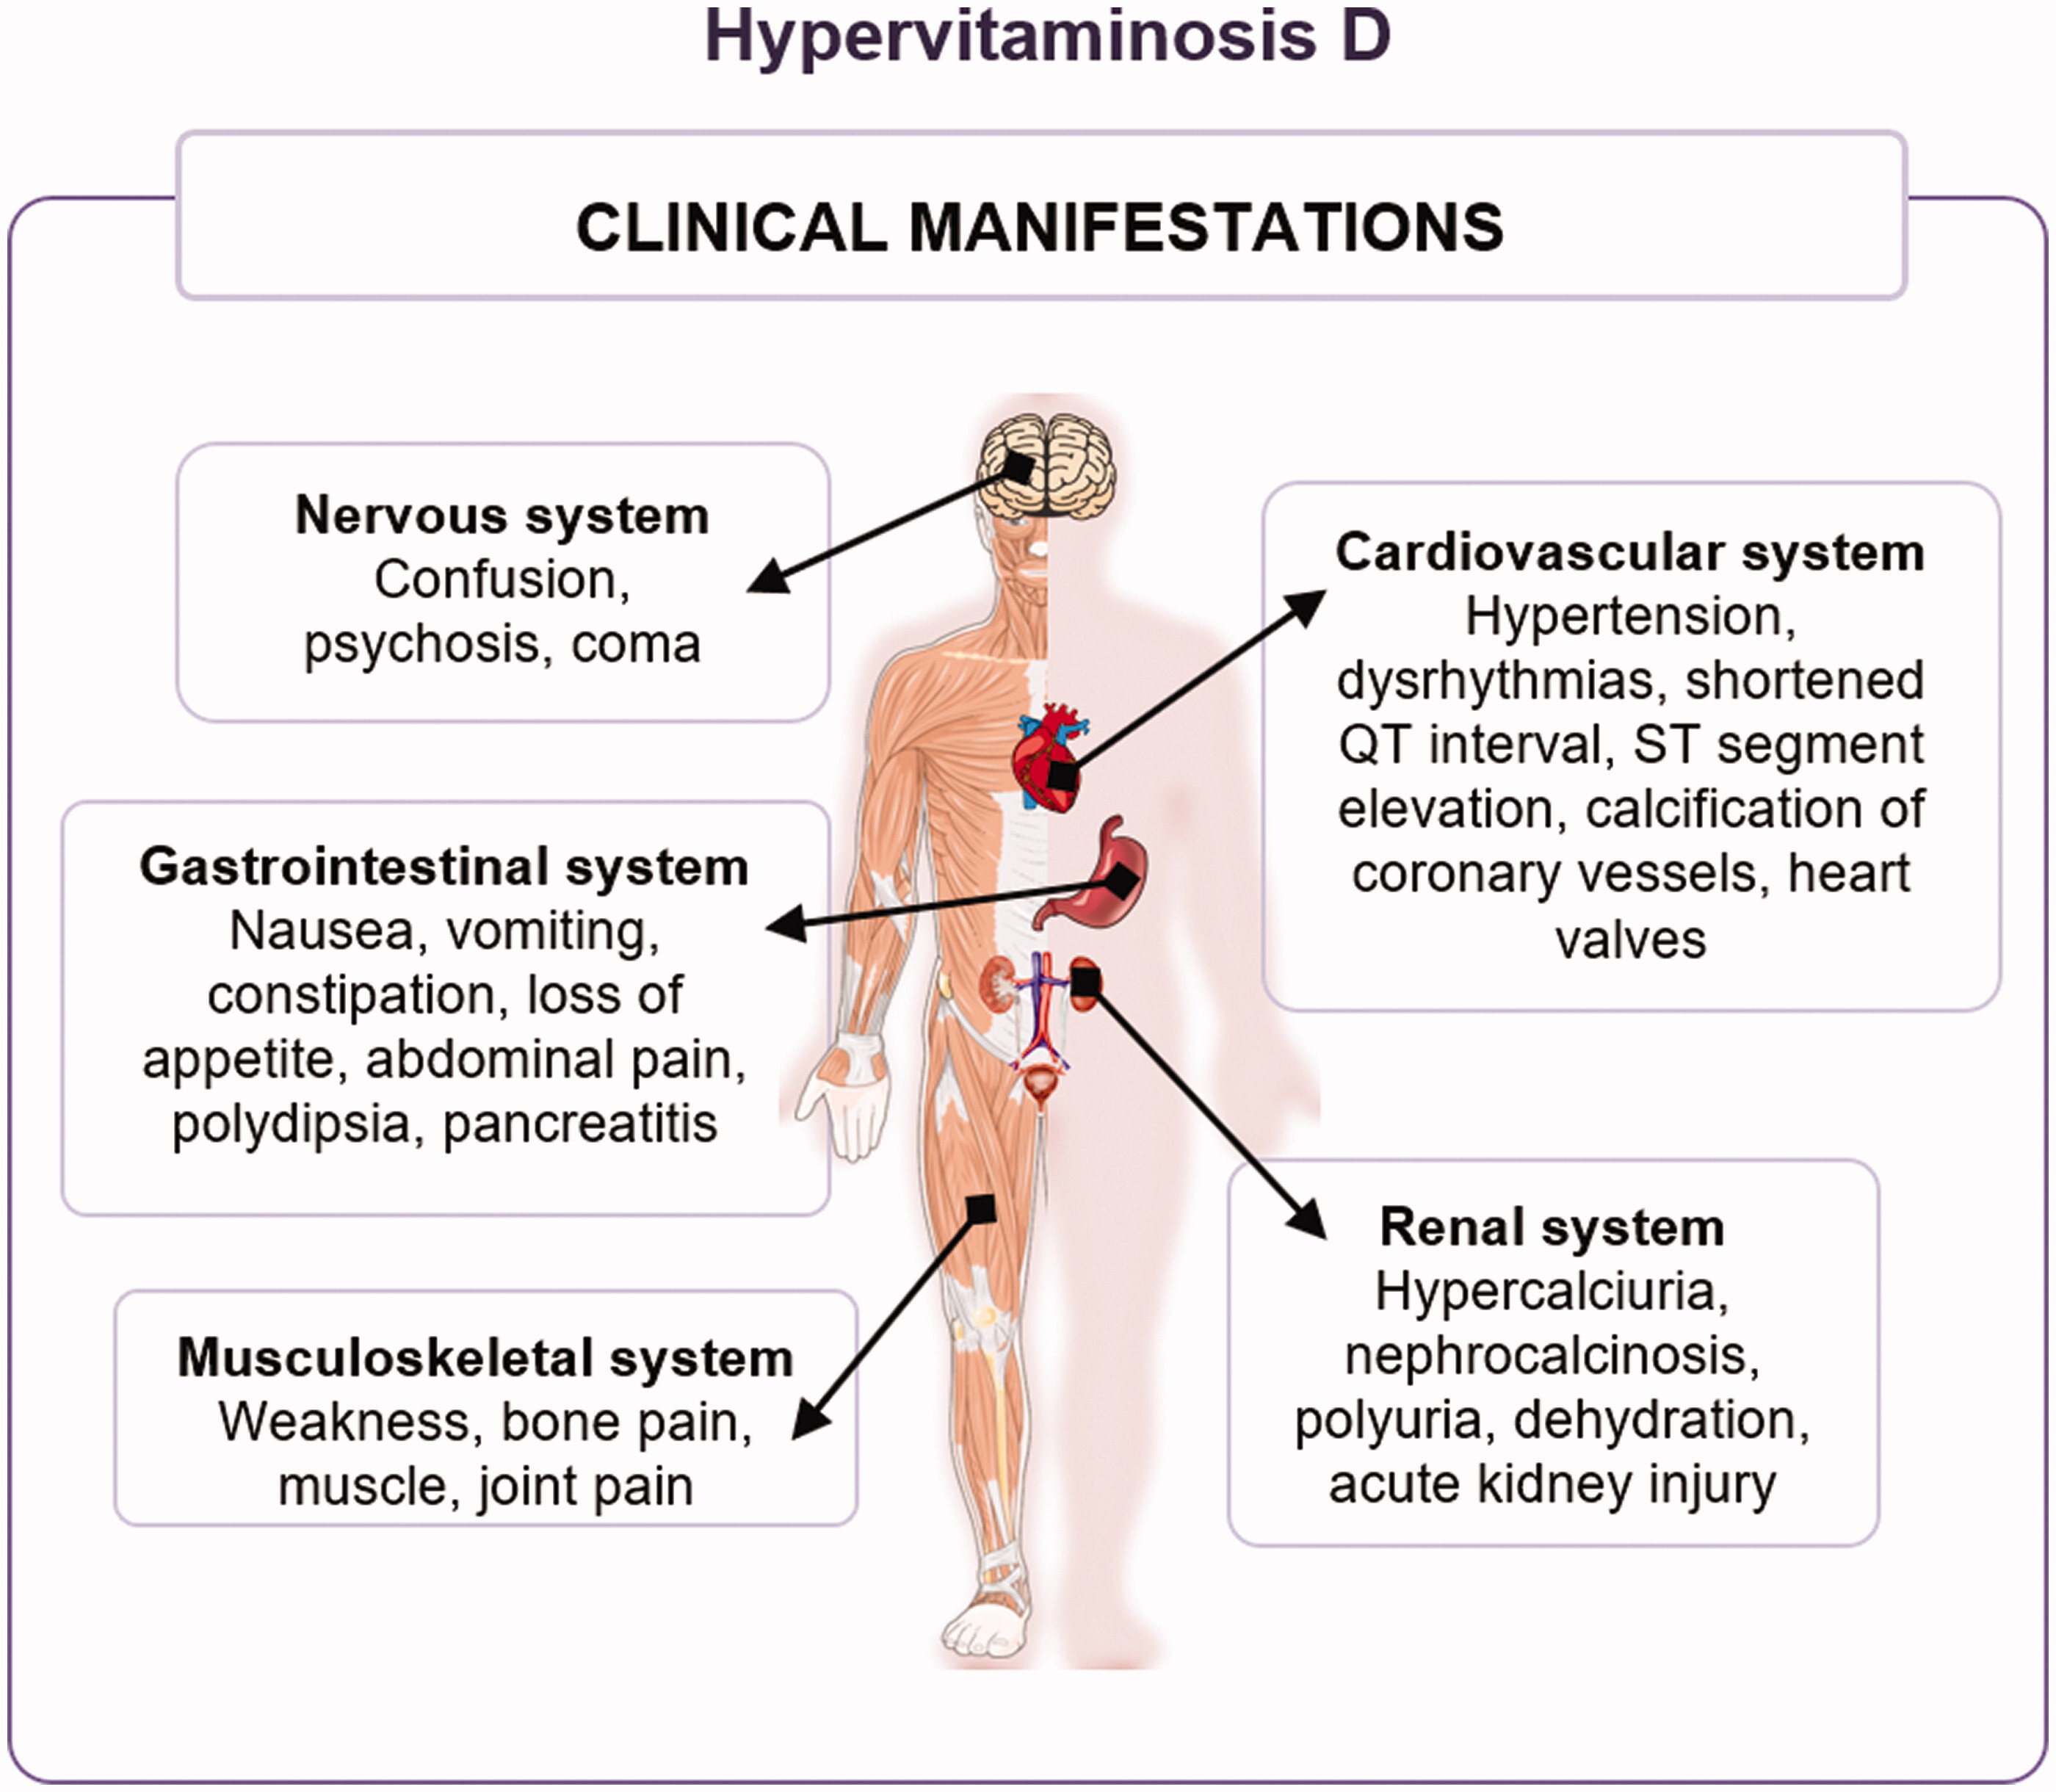
\includegraphics{figures/hypervitaminosis-d.jpg}

}

\caption[Symptômes associés lors d'une hypervitaminose
D.]{\label{fig-hypervitaminose-d}\textbf{Symptômes associés lors d'une
hypervitaminose D} \autocite{Janoušek.2022}.}

\end{figure}%

La toxicité de la vitamine D est habituellement d'origine iatrogène, le
surdosage de vitamine D pouvant être accidentel, conséquence d'une
erreur médicale ou d'un malentendu sur des recommandations médicales
\autocite{Lim.2020vd}. Elle peut aussi résulter d'une activité excessive
de la production endogène anormale de calcitriol par les macrophages
chez les patients lors de maladies granulomateuses comme la sarcoïdose,
les maladies fongiques, la lèpre et la bérylliose
\autocite{Marcinowska-Suchowierska.2018}. Il peut exister enfin des
situations d'excès de \ac{25(OH)D3} et de \ac{1,25(OH)2D3} dans des
troubles congénitaux, tels que le syndrome de Williams-Beuren, qui
s'accompagne d'une déficience en 24-hydroxylase, et donc ne permet pas
la métabolisation de \ac{25(OH)D3} and \ac{1,25(OH)2D3} en métabolites
inactifs \autocite{Marcinowska-Suchowierska.2018}. Ce syndrome cause
ainsi hypercalcémie, néphrolithiase, et néphrocalcinose
\autocite{Azer.2021}.

\subsection{Seuil de toxicité actuel}\label{seuil-de-toxicituxe9-actuel}

L'\ac{IOM} a fixé à 4000 UI/j de cholécalciférol la limite supérieure de
sécurité, c'est-à-dire la dose maximale pouvant être consommée sans
risque de façon chronique. Ce seuil a été établi en considérant un
apport de 10 000 UI/j de cholécalciférol comme le nouveau d'apport le
plus élevé non associé à des effets négatifs et en tenant compte des
incertitudes sur des données comme la mortalité toute causes, pour des
prises inférieures à 10 000 UI/j. La limite supérieure de sécurité
concerne également les enfants de 9 à 18 ans mais est réduite pour les
enfants de 1 à 8 ans (2500 à 3000 UI/j). Cependant l'IOM admet que les
signes de toxicité de la vitamine D sont rares pour une valeur de 10 000
UI/j, mais que la toxicité est plus commune vers des doses de 50 000
UI/j . Ces valeurs sont toutefois basées sur des données limitées et des
études supplémentaires sont nécessaires pour déterminer les effets de la
vitamine D sur la santé au-delà de ces valeurs \autocite{IOM.2011}.

L'ANSM a publié un avis sur le bon usage de la vitamine D, suite à des
cas rapportés de surdosage de vitamine D entraînant une hypercalcémie,
parfois accompagnée de lithiase et néphrocalcinose chez des enfants et
des nourrissons, après avoir pris une dose plus de deux fois supérieure
à la dose recommandée (400 UI par jour de 0 à 18 ans chez l'enfant en
bonne santé sans facteur de risque, 800 UI par jour de 0 à 18 ans chez
l'enfant présentant un facteur de risque) pendant plusieurs semaines, et
deux cas d'intoxication sévère à la vitamine D après avoir pris un
complément alimentaire acheté sur internet contenant une dose de 10 000
UI par goutte \autocite{ANSM.2021}.

--\textgreater{}

\newpage{}

\chapter{Vitamine D, système immunitaire et réponse
antivirale}\label{vitamine-d-systuxe8me-immunitaire-et-ruxe9ponse-antivirale}

L'importance du rôle de la vitamine D sur le système immunitaire a
récemment retenu l'attention des chercheurs depuis la découverte de la
coexistence du \ac{VDR} et du \ac{CYP27B1} dans des tissus dont la
fonction n'est pas directement liée à l'homéostasie du calcium
\autocite{Zehnder.2001}. En particulier, l'expression du \ac{CYP27B1}
dans les cellules immunitaires est régulée indépendamment de
l'homéostasie du calcium \autocite{White.2022}. Deux observations
principales suggèrent un rôle de la vitamine D dans le système
immunitaire : le \ac{VDR} est présent dans toutes les cellules
immunitaires, et la présence du \ac{CYP27B1} est induite par certaines
cellules immunes \autocite{Giannini.2022}. De ce fait, cette découverte
de la présence de CYP27B1 extra-rénale suggère un rôle local de l'action
paracrine ou intracrine du calcitriol
\autocite{Hewison.2007,Bishop.2021}.

La vitamine D agit à la fois sur le système immunitaire inné et
adaptatif (\Cref{fig-vd-immune-effect}). En effet, par le biais de la
synthèse intracrine du calcitriol par les macrophages et cellules
dendritiques, le calcitriol est active en amont et en aval des \acp{PRR}
qui jouent un rôle initial dans la réponse innée, stimule la production
de peptides antimicrobiens et en particulier la cathélicidine dont il
est un puissant inducteur, diminue les concentrations de fer via
l'induction de l'hepcidine, augmente l'autophagie permettant de
combattre les pathogènes intracellulaires tels que \emph{M.
tuberculosis} \autocite{Liu.2006}, et les infections virales, et joue un
rôle important dans le système adaptatif par une suppression des
réponses cellulaires \ac{Th1} et \ac{Th17} tout en promotant une
immunotolérance \autocites[ ]{Bishop.2021}{Ismailova.2022}.

Ainsi, plusieurs cellules immunitaires peuvent synthétiser l'enzyme clé
permettant la conversion du \ac{25(OH)D3} en \ac{1,25(OH)2D3}, le
cytochrome \ac{CYP27B1} ou aussi appelée 1α-hydroxylase. L'induction de
cette enzyme concerne des cellules telles que les cellules dendritiques,
monocytes, macrophages, lymphocytes B et T
\autocite{Giannini.2022,Dankers.2017}.

Dans ce contexte, l'enzyme 1α-hydroxylase n'est pas uprégulée par la
\ac{PTH}. Par conséquent, la production de \ac{1,25(OH)2D3} dépend des
niveaux de substrat de \ac{25(OH)D3} et peut être régulée par des
signaux inflammatoires, tels que le \ac{LPS} et les cytokines
\autocite{Giannini.2022}.

\section{Mécanismes d'action de la vitamine D sur le système
immunitaire}\label{muxe9canismes-daction-de-la-vitamine-d-sur-le-systuxe8me-immunitaire}

Comme nous allons le voir, la vitamine D possède une action globalement
anti-inflammatoire et donc régulatrice de l'inflammation
(\Cref{fig-vd-immune-effect}). Elle agit à la fois sur le système
immunitaire inné et adaptatif. A l'initiation de la réponse
inflammatoire, le calcitriol est essentiel afin de répondre à une
infection. Les effets de la vitamine D ne répriment pas totalement le
système immunitaire mais plutôt induit une modulation immunitaire, en
faisant évoluer le système immunitaire adaptatif vers une tolérance
antigénique, et le système immunitaire inné vers une meilleure
élimination virale et bactérienne \autocite{Martens.2020}. Le calcitriol
n'est donc pas purement anti-inflammatoire mais il contribue à maintenir
l'équilibre entre un état pro- et anti-inflammatoire et est donc capable
de rétablir l'équilibre perturbé \autocite{Dankers.2017}.

\begin{figure}

\centering{

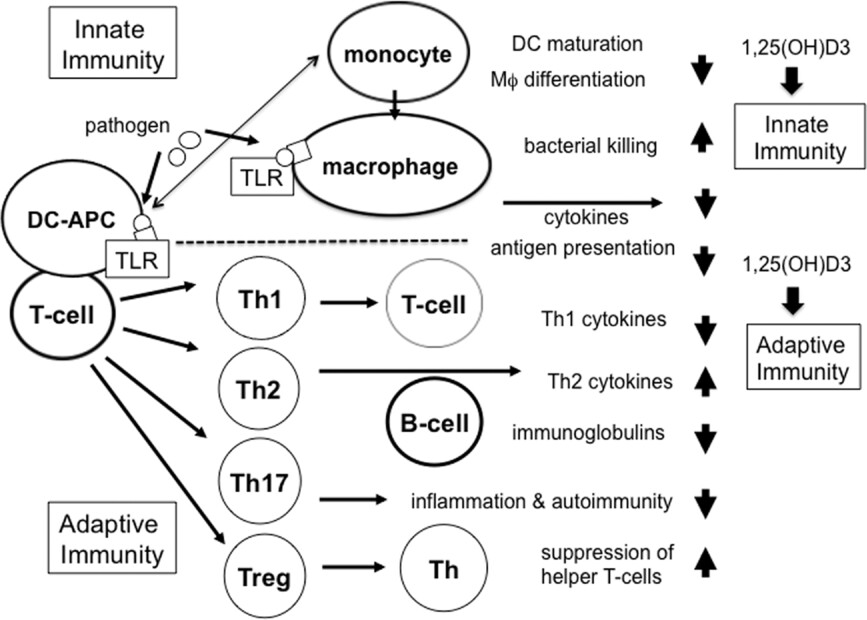
\includegraphics{figures/vd-immune-effect.jpg}

}

\caption[Effets du calcitriol sur la réponse
immunitaire.]{\label{fig-vd-immune-effect}\textbf{Effets du calcitriol
sur la réponse immunitaire.} La \ac{1,25(OH)2D3} régule à la fois
l'immunité innée et l'immunité adaptative, en potentialisant l'activité
antimicrobienne des macrophages, en diminuant la présentation de
l'antigène et en diminuant les fonctions des lymphocytes B et de
certains lymphocytes T. Cependant, dans des conditions normales, la
\ac{1,25(OH)2D3} augmente le phénotype \ac{Th2} des lymphocytes T helper
et l'efficacité des \ac{Treg}. DC, cellules dendritiques ; APC, cellules
présentatrices d'antigènes ; \acs{TLR}, \acl{TLR} ; \ac{Treg},
\acl{Treg}. D'après \textcite{Cutolo.2014}}

\end{figure}%

\subsection{Action intracrine et
autocrine}\label{action-intracrine-et-autocrine}

Les études suggèrent que la vitamine D délivre ses effets par un
mécanisme intracrine ou autocrine et non systémique au sein des tissus
non-classiques \autocite{Hewison.2007} et agit localement dans les
cellules immunitaires. Un mécanisme intracrine se réfère à un mécanisme
impliquant une molécule agissant et produite par la même cellule. En
effet, trois aspects spécifiques de la \ac{CYP27B1} ont attiré
l'attention des chercheurs : l'expression et la régulation dans les
tissus non classiques au cours de la physiologie normale ; les effets
sur le système immunitaire et les maladies inflammatoires ; l'expression
et la fonction dans les tumeurs.

\textcite{Hewison.2007} investigue l'idée d'un mécanisme extra-rénal de
\ac{CYP27B1} rapporté dans la littérature et l'efficacité de la réponse
du calcitriol endogène dans la modulation de la réponse immune. En
représentant les conditions de carence en vitamine D, d'insuffisance en
vitamine D et de suffisance en vitamine D, par une dose de 5, 50 and 150
nM respectivement, l'accumulation de calcitriol dans les cellules
dendritiques et macrophages et d'un inhibiteur de CYP27B1, est due à
l'activité de l'enzyme 1α-hydroxylase et est augmenté, lorsque les
concentrations de calcidiol augmentent, et impacte selon une relation
dose-réponse la stimulation de CD14 et la répression de marqueurs de
cellule dendritique CD86, CD83 et HLA-DR.

Similairement, l'essai \emph{in vitro} de \textcite{Adams.2009} montre
que le calcidiol est nécessaire pour produire la cathélicidine et
qu'elle est dépendante de l'expression du CYP27B1 du macrophage, bien
qu'à haute concentration le calcidiol peut stimuler la production de
cathélicidine sans passer par l'activation des macrophages via le
\ac{TLR} De plus, l'expression de cathélicidine est fortement diminuée
lorsque la concentration de vitamine D administrée est inférieure à 30
ng/mL. En outre, les auteurs ont observé une absence de corrélation
entre les niveaux de cathélicidine plasmatique et les niveaux de
calcidiol plasmatique, ainsi que la concentration de cathélicidine
leucocytaire et la concentration plasmatique de calcidiol, ce qui
suggère que l'effet de la vitamine D sur la synthèse de la cathélicidine
par les cellules immunes est due non pas à la présence de calcidiol
plasmatique mais bien à l'effet local intracrine des cellules immunes.

\textcite{Chun.2010} a montré que la concentration de calcitriol dans
les monocytes était de 10-100 fois plus élevée que dans le plasma, ce
qui suggère que la concentration locale de calcitriol est beaucoup plus
élevée que la concentration plasmatique. Cela suggère que la vitamine D
peut agir de manière intracrine.

L'effet autocrine de la vitamine D sur des lymphocytes T
CD4\textsuperscript{+} a été observé par \textcite{Chauss.2022}.
L'administration de calcitriol actif ou calcidiol conduit aux cellules à
réprimer l'\ac{ifng} et augmenter la synthèse d'\ac{IL-10}, indiquant
que les cellules ont acquises la capacité de métaboliser et de répondre
aux métabolites de la vitamine D. Inversement, lors du KO d'un des gènes
concernant la vitamine D tel que \emph{CTSL}, \emph{VDR} ou
\emph{CYP27B1}, une réduction nette en \ac{IL-10} est observée. Dans
l'ensemble les résultats indiquent l'effet d'un mécanisme
intracellulaire autocrine/paracrine de la vitamine D. Des résultats
similaires ont été retrouvé par \textcite{Adams.2009} par le KO du
\emph{VDR} et \emph{CYP27B1} et l'expression de la cathélicidine
diminuée.

\subsection{Induction de l'immunité innée
antimicrobienne}\label{induction-de-limmunituxe9-innuxe9e-antimicrobienne}

Après l'entrée du calcitriol dans la cellule ou la conversion du
calcidiol en calcitriol intracellulaire, l'action du calcitriol est
médié par l'hétérodimère \ac{VDR}-\ac{RXR} et se fixe sur le \ac{VDRE},
causant la régulation de multiples gènes
(\Cref{fig-vd-immune-signaling}) \autocite{Caprio.2017,Yasmin.2005}. Un
des mécanismes principaux de l'immunité innée antimicrobienne passe par
l'induction de peptides antimicrobiens et en particulier la forte
induction de cathélicidine \autocite{Wang.2004}. En effet, la vitamine D
stimule l'expression du gène \emph{CAMP} en se liant au \ac{VDRE} situé
son promoteur et induit la cathélicidine humaine hCAP-18, clivant ce
précurseur en LL-37 par la protéinase 3. Le domaine C-terminal de hCAP18
nommé LL-37, est un peptide antimicrobien qui déstabilise les membranes
bactériennes et fongiques et peut empêcher la réplication virale en se
liant aux protéines de pointes \autocite{Bishop.2021,Charoenngam.2020}.
De plus, LL-37 est impliqué dans la signalisation, induisant la
chimiotaxie et participe à la régénération tissulaire et est capable
d'activer les TLR7 et TLR8 activant la cellule dendritique
\autocite{Silva.2012}. Le LL-37 est exprimé par les leucocytes,
notamment les neutrophiles, les monocytes, les mastocytes, les cellules
NK, les lymphocytes T et B. Le LL-37 a également été trouvé dans le
plasma, la moelle osseuse, les voies respiratoires, l'intestin, les
glandes mammaires, l'épididyme et la peau \autocite{Silva.2012}. De
plus, le calcitriol induit également la défensine \mupbeta 2 et par le
gène \emph{HBD2} qui contribue à la défense antimicrobienne.

\begin{figure}

\centering{

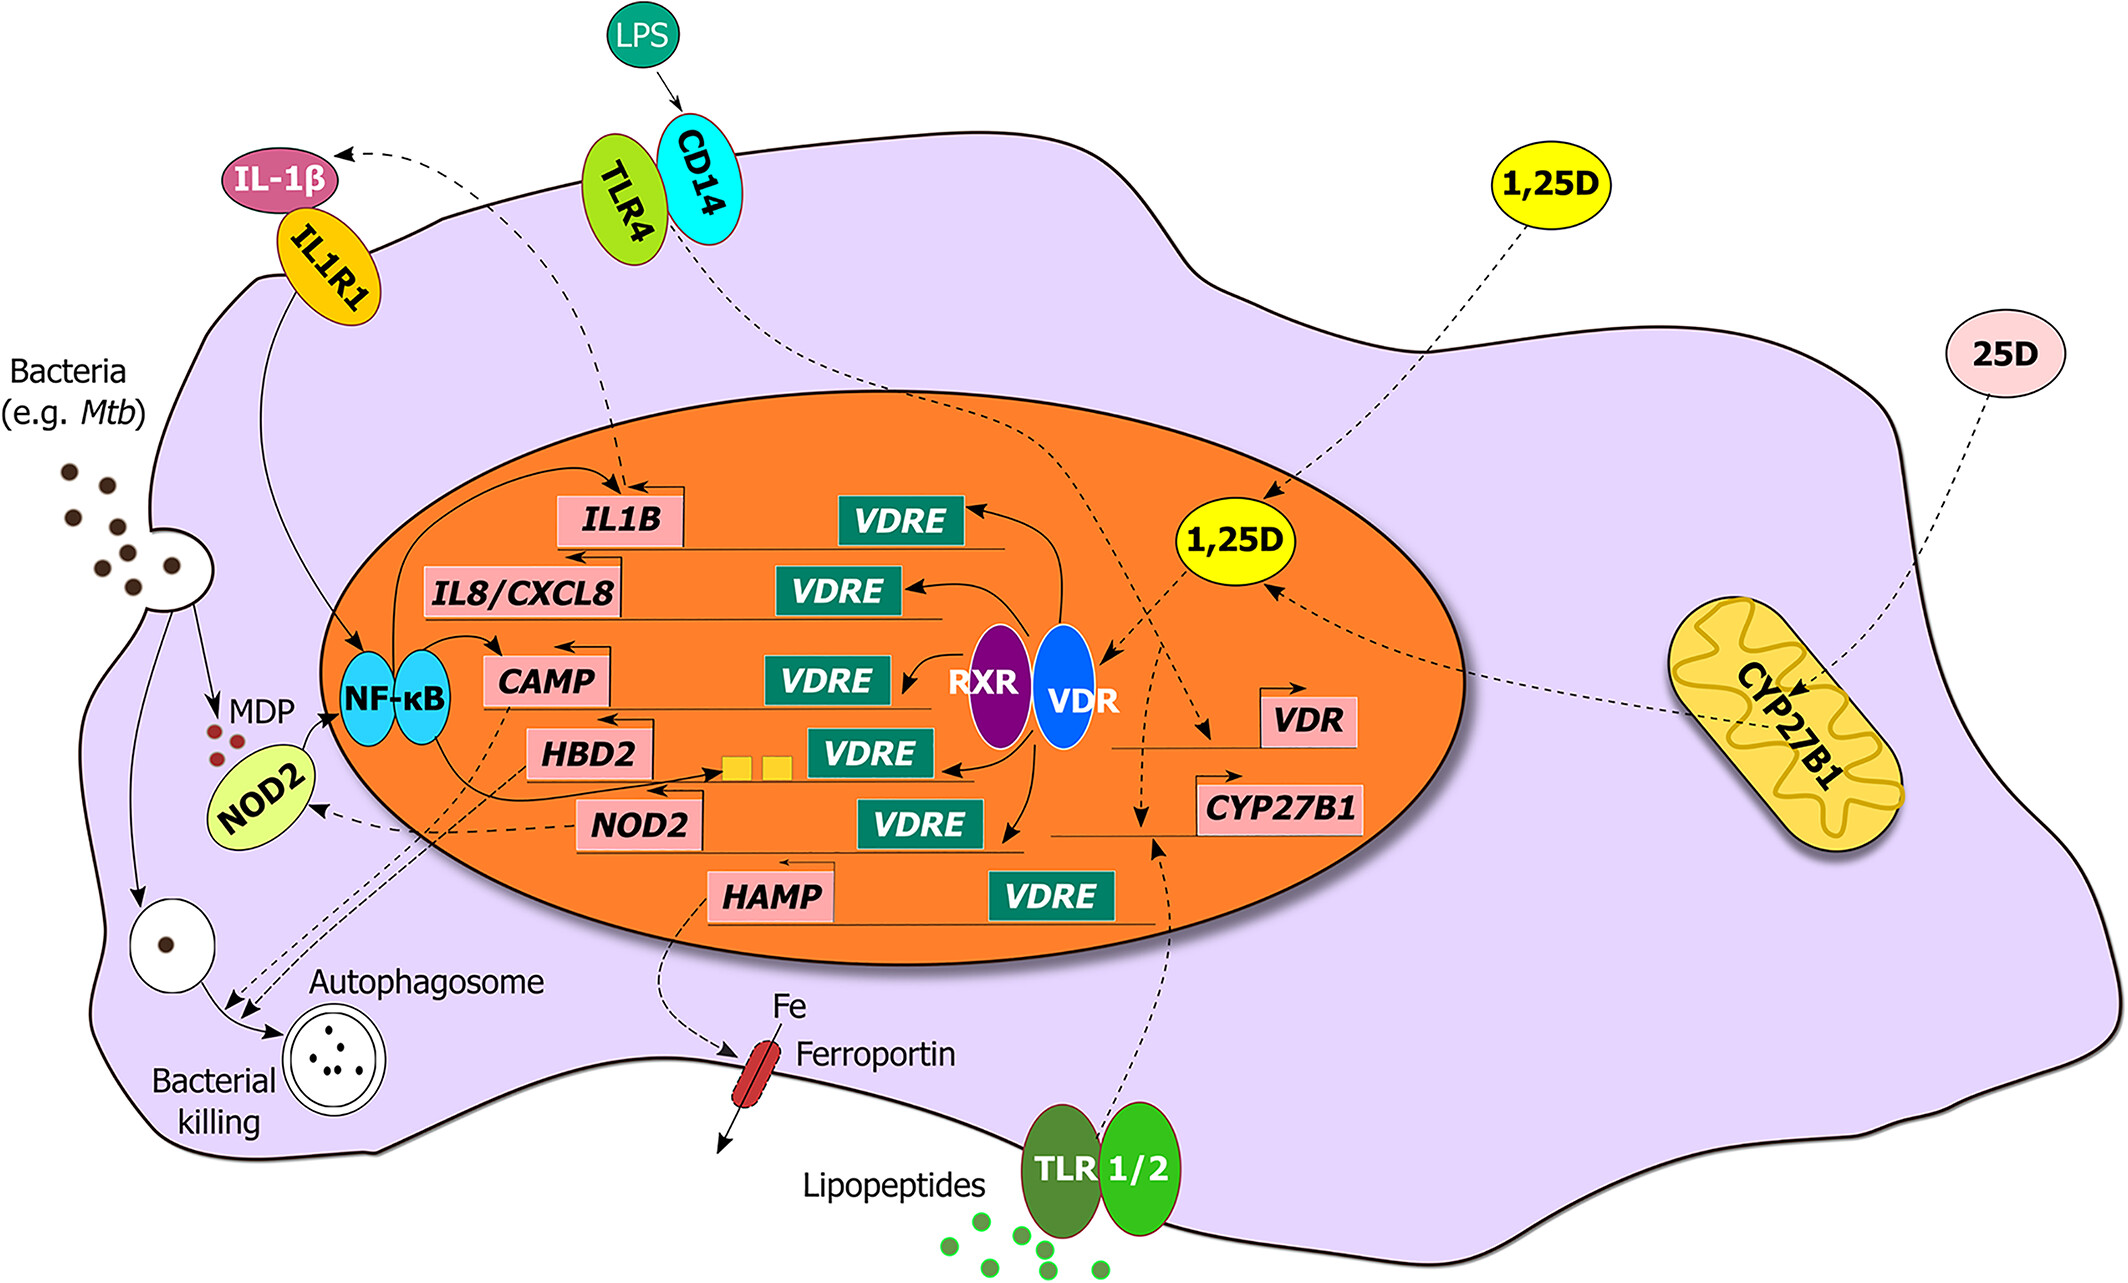
\includegraphics{figures/Ismailova.2022-Vitamin_D_metabolism_and_innate_immune_signaling_in_the_monocyte-macrophage.jpg}

}

\caption[Métabolisme de la vitamine D et signalisation immunitaire innée
dans le
monocyte/macrophage.]{\label{fig-vd-immune-signaling}\textbf{Métabolisme
de la vitamine D et signalisation immunitaire innée dans le
monocyte/macrophage.} Après liaison du calcitriol sur le VDR, le
complexe VDR-RXR se lie sur différentes séquences \ac{VDRE} spécifiques,
induisant l'expression de peptides antimicrobiens tel que la
cathélicidine et la défensine \mupbeta 2, diminue l'expression de
l'hepcidine, favorise l'autophagie, l'expression de PRR et de cytokines
\autocite{Ismailova.2022}.}

\end{figure}%

En réponse au calcitriol, le \ac{VDR} induit l'expression des \ac{PRR}
NOD2, des peptides antimicrobiens comme la cathélicidine et défensine
\mupbeta 2, et des cytokines IL-1β et IL-8
(\Cref{fig-vd-immune-signaling}). Le complexe calcitriol-VDR a également
pour fonction de supprimer l'expression de \emph{HAMP}, ce qui entraîne
une augmentation de l'exportation du fer médiée par la ferroportine. En
effet, presque tous les microorganismes utilisent le fer pour leur
croissance. De ce fait, la restriction du fer par l'organisme constitue
une des réponses afin de lutter contre l'infection ; l'expression de
\emph{HAMP} est augmentée lors de stimuli bactériens et viraux
\autocite{Bishop.2021}. Lors de la stimulation par le ligand muramyl
dipeptide (MDP) généré par la décomposition du peptidoglycane bactérien,
NOD2 et IL-1β peuvent augmenter l'expression de \emph{HBD2}, \emph{CAMP}
et \emph{IL1B} \autocite{Bishop.2021}.

\subsection{Effets immunomodulateurs}\label{effets-immunomodulateurs}

\subsubsection{Macrophages et monocytes}\label{macrophages-et-monocytes}

Le calcitriol induit le switch phénotypique de macrophage M1 vers M2 par
la régulation positive de l'\ac{IL-10}. Le macrophage M2 est un type de
macrophage ayant un profil anti-inflammatoire contrairement au
macrophage M1 au profil pro-inflammatoire. Le calcitriol inhibe
également des cytokines majeures pro-inflammatoires telles que
l'\ac{IL-6} et le \ac{tnfa} \autocite{Meza-Meza.2022,Caprio.2017}. Il a
également été démontré que le calcitriol supprime l'expression des
\ac{TLR} sur les monocytes et inhibe la production des cytokines
inflammatoires \ac{IL-2}, l'\ac{IL-6} et l'\ac{IL-17}. La vitamine D
stimule également le signalement cytokinique, avec induction de
chimiokines comme l'IL-8/CXCL8, une chimiokine agissant sur le
neutrophile.

Comme discuté précédemment, les effets du calcitriol ne sont pas
toujours de nature pro-inflammatoire. La vitamine D possède un pouvoir
pro-inflammatoire dans la réponse initiale de l'inflammation, puis un
pouvoir anti-inflammatoire lors de la phase de résolution de
l'inflammation \autocite{Dankers.2017}. En effet, la culture de
monocytes avec le \ac{LPS} montre une répression de l'\ac{IL-10} pendant
les 8 premières heures, suivie d'une induction 48 heures après la
réponse initiale \autocite{Matilainen.2010}.

\begin{figure}

\centering{

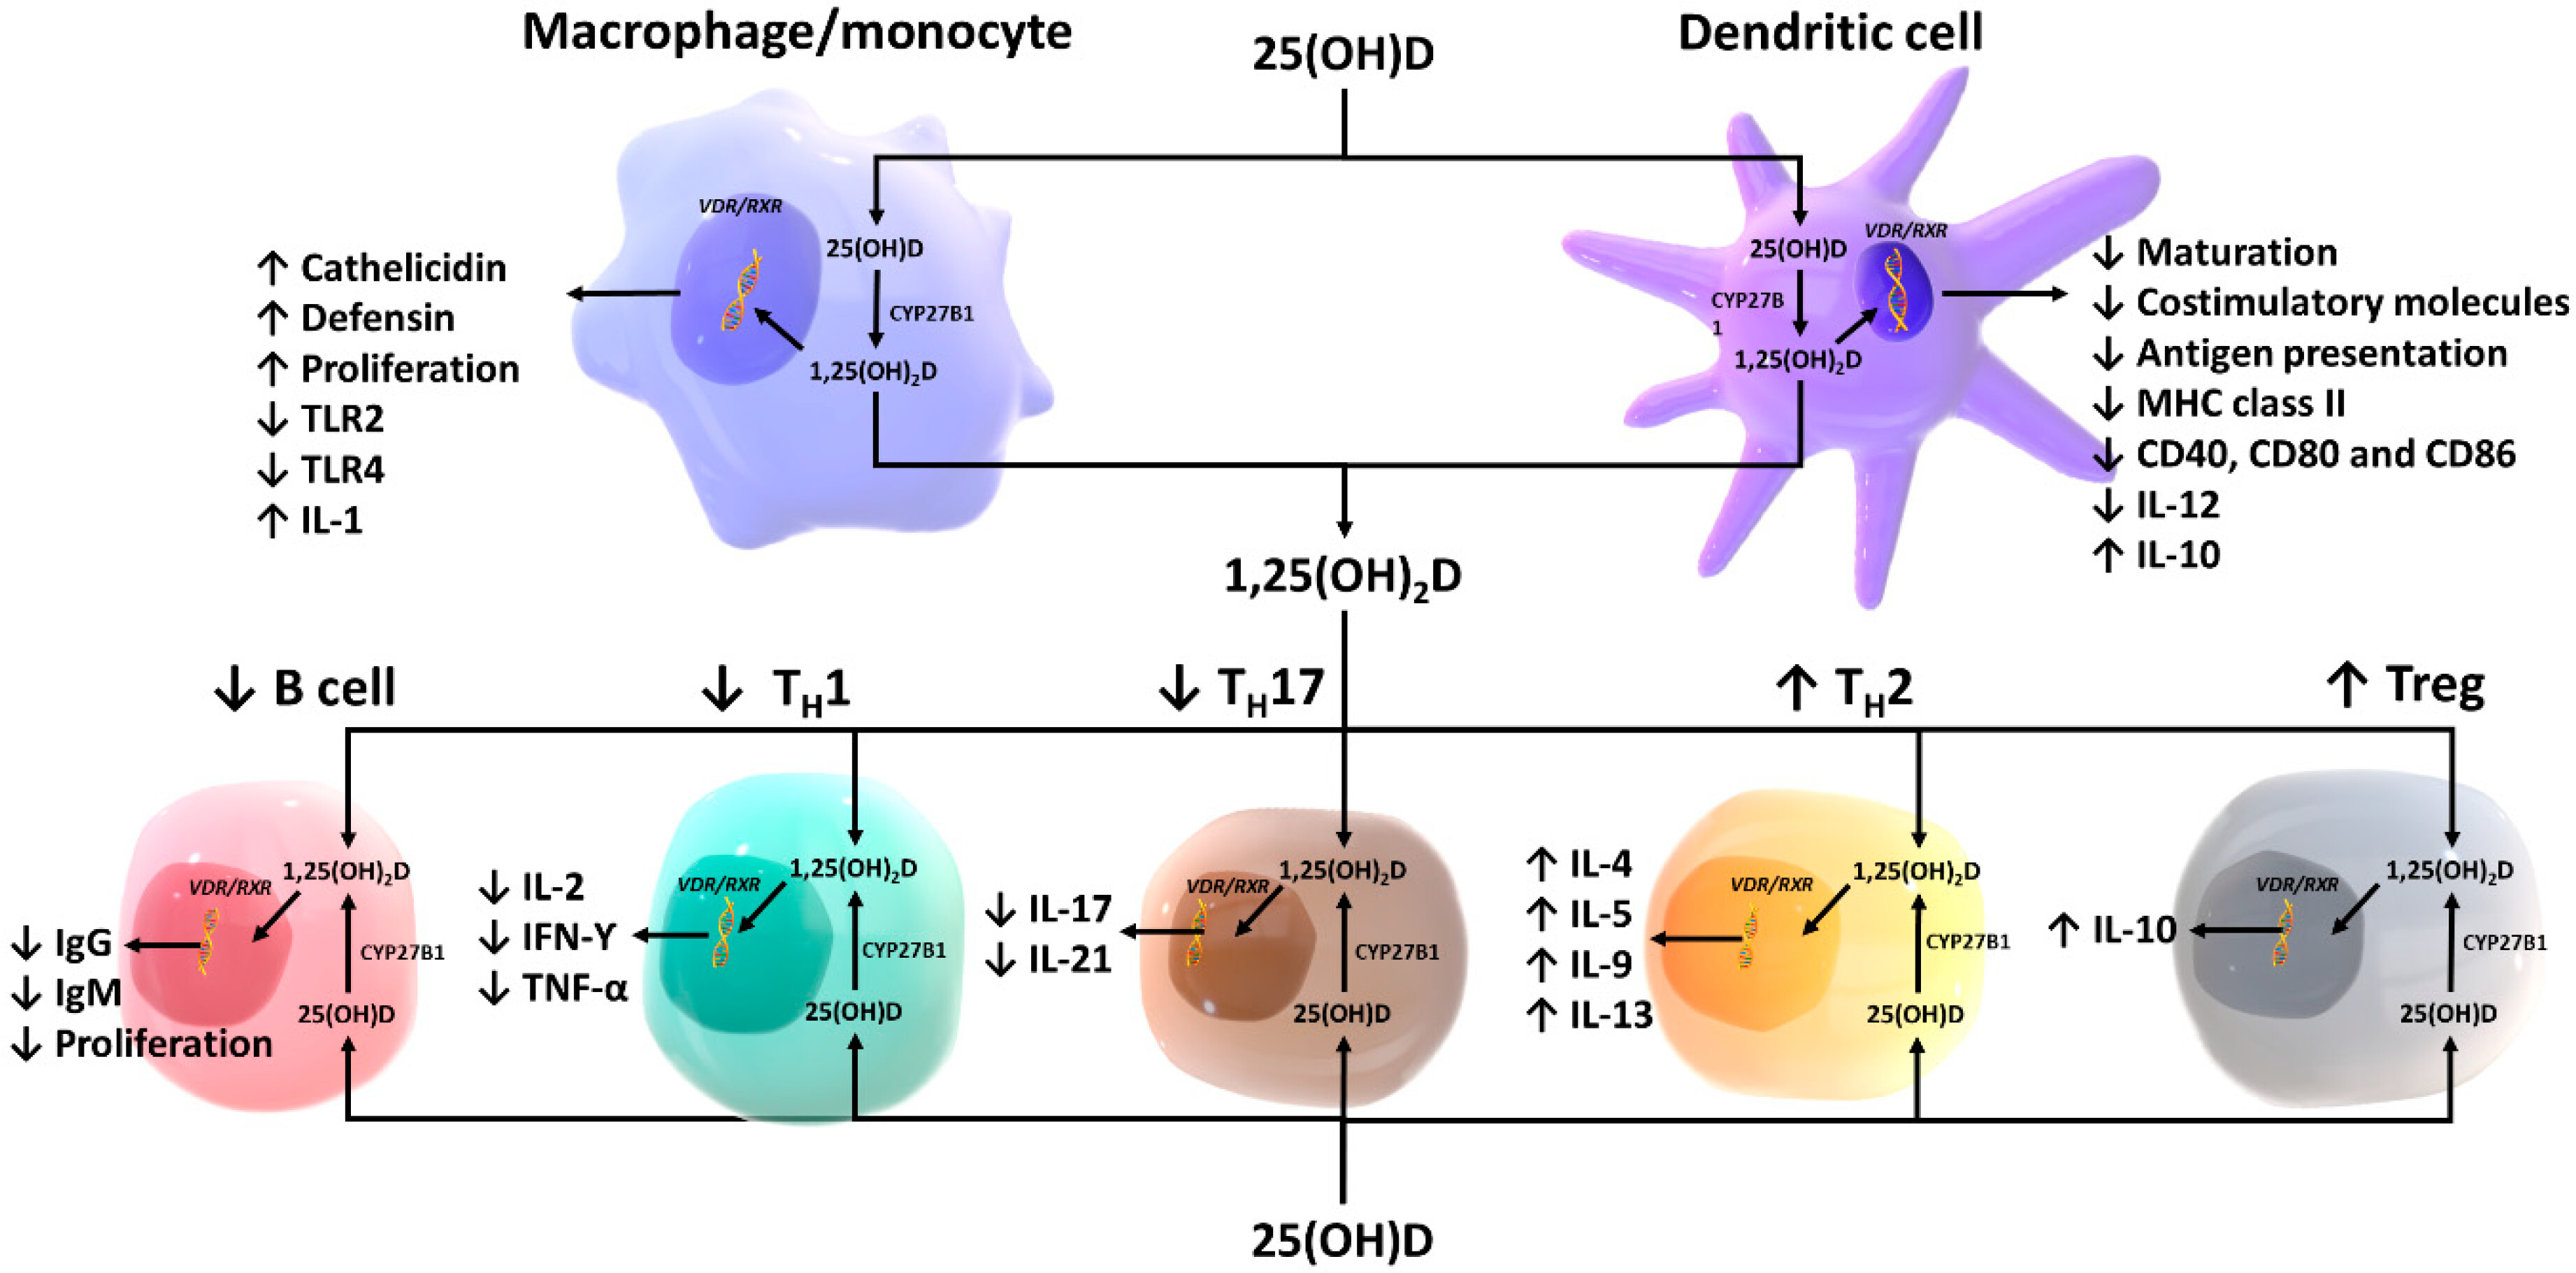
\includegraphics{figures/vd-action.jpg}

}

\caption[Représentation schématique des fonctions paracrine et
intracrine de la vitamine D et de ses métabolites et des actions de la
\ac{1,25(OH)2D3} sur les systèmes immunitaires innés et
adaptatifs.]{\label{fig-vd-action}\textbf{Représentation schématique des
fonctions paracrine et intracrine de la vitamine D et de ses métabolites
et des actions de la \ac{1,25(OH)2D3} sur les systèmes immunitaires
innés et adaptatifs.} Les macrophages, monocytes et cellules
dendritiques sont capables d'induire le \ac{CYP27B1} afin de métaboliser
le calcidiol en calcitriol, qui va ensuite agir de manière intracrine
par le biais de la translocation de l'hétérodimère \ac{VDR}-\ac{RXR} et
agir directement sur l'expression des facteurs de transcription.
Globalement les effets issus du calcitriol seront liés à l'augmentation
de la défense innée notamment par le biais de la cathélicidine, ainsi
qu'une diminution du phénotype mature de la cellule dendritique et une
augmentation du phénotype tolérogène. Par la suite, le calcitriol peut
agir sur les cellules environnantes en favorisant un phénotype
anti-inflammatoire chez les cellules \ac{Th2} et \ac{Treg} ainsi qu'une
diminution de l'activation des cellules \ac{Th1} et \ac{Th17}, et des
cellules B. Abréviation : \ac{1,25(OH)2D3} : \acl{1,25(OH)2D3} ;
\ac{25(OH)D3} : \acl{25(OH)D3} ; \ac{ifng} : \acl{ifng} ; IL :
interleukine ; CMH : complexe majeur d'histocompatibilité ; RXR :
\acl{RXR} ; Th1 : T helper 1 ; Th2 : T helper 2 ; Th17 : T helper 17 ;
\ac{Treg}, \acl{Treg} ; \ac{tnfa}, \acl{tnfa} ; \ac{TLR}, \acl{TLR}
\ac{VDR}, \acl{VDR}. \autocite{Charoenngam.2020}}

\end{figure}%

\subsubsection{Cellules présentatrices d'antigènes et lymphocytes
NK}\label{cellules-pruxe9sentatrices-dantiguxe8nes-et-lymphocytes-nk}

Le calcitriol agit également sur les \ac{CPA} : cellules dendritiques,
macrophages, lymphocytes B, et \ac{NK} en les rendant plus immature et
tolérogéniques, par le biais d'une diminution de l'expression de
\ac{CMH-II} qui leur permet de présenter des antigènes étrangers, ainsi
que l'expression de molécules de co-stimulation (\ac{CD} 40, CD80, CD86)
qui jouent un rôle essentiel dans la stimulation des lymphocytes
(\Cref{fig-vd-action})
\autocite{Charoenngam.2020,Meza-Meza.2022,Caprio.2017}. Ce changement
phénotypique s'accompagne donc d'une diminution de la capacité de
présentation d'antigènes et de production d'\ac{IL-12}, interleukine clé
pour la différenciation des lymphocytes T en Th1, l'activité cytotoxique
des lymphocytes \ac{NK} et lymphocytes CD8\textsuperscript{+}, ainsi
qu'une augmentation d'\ac{IL-10}, une cytokine clé dans la régulation du
système immunitaire.

En outre, des études expérimentales ont suggéré que la différenciation
et la fonction des lymphocytes \ac{NK} peuvent être modulées par un
traitement au calcitriol \autocite{Charoenngam.2020}. Cependant, le rôle
inducteur ou inhibiteur du calcitriol est encore indéterminé par manque
de données cohérentes.

La vitamine D joue un rôle essentiel dans la modulation des réponses
immunitaires adaptatives, en particulier des lymphocytes T et B, qui
sont les principales cellules immunitaires de cette composante du
système immunitaire. Les lymphocytes T sont impliqués dans la
reconnaissance des antigènes et la destruction des cellules infectées ou
tumorales, tandis que les lymphocytes B sont impliqués dans la
production d'anticorps. La vitamine D agit sur ces deux types de
lymphocytes en modulant leur fonctionnement et leur activation. La
vitamine D est notamment importante comme élément régulateur entre les
réponses immunitaires pro-inflammatoires et anti-inflammatoires.

Il a été observé que les lymphocytes n'expriment que faiblement le
\ac{VDR} à l'état basal, contrairement aux monocytes, mais fortement
après activation. Les lymphocytes activés expriment également le
\ac{CYP27B1} nécessaire pour convertir le calcidiol en calcitriol
\autocite{Charoengramm.2020}

\subsubsection{Lymphocytes T}\label{lymphocytes-t}

Les lymphocytes T sont composés en plusieurs sous-groupes :

\begin{itemize}
\item
  les lymphocytes T auxiliaires ou helper CD4\textsuperscript{+} Th1,
  Th2, Th17. Les populations \ac{Th1} et \ac{Th17} ont principalement
  pour rôle de stimuler une réponse cytotoxique, respectivement
  intracellulaire antibactérienne et antiprotozoaire comme le
  toxoplasme, et extracellulaire antibactérienne et fongique. La
  population \ac{Th2} en revanche est centrée sur une stimulation de la
  réponse humorale ou médiée par les anticorps, contre les parasites
  extracellulaires, les bactéries, les allergènes et les toxines, médiée
  par le biais de cytokines causant une forte production d'anticorps,
  l'activation des éosinophiles et de l'inhibition de plusieurs
  fonctions des macrophages
\item
  les lymphocytes T effecteurs CD8\textsuperscript{+} capables d'induire
  la mort des cellules.
\item
  les lymphocytes T CD4\textsuperscript{+} régulateurs ou \ac{Treg}, qui
  ont pour rôle de réguler l'inflammation et donc la réponse
  immunitaire.
\end{itemize}

lymphocytes T auxiliaires ou helpers \acs{Th} type
CD4\textsuperscript{+} (Th\textsubscript{1}, Th\textsubscript{2},
Th\textsubscript{17}), et les lymphocytes T CD8\textsuperscript{+} qui
sont les lymphocytes effecteurs capables d'induire l'apoptose des
cellules. La population Th\textsubscript{1} et Th\textsubscript{17} a
principalement pour rôle de stimuler une réponse cytotoxique, en
stimulant respectivement les macrophages pour une réponse
intracellulaire antibactérienne et antiprotozoaire comme le toxoplasme,
et les neutrophiles pour une réponse extracellulaire antibactérienne et
fongique. La population Th\textsubscript{2} en revanche est centrée sur
une stimulation de la réponse humorale ou médiée par les anticorps,
contre les parasites extracellulaires, les bactéries, les allergènes et
les toxines, médiée par le biais de cytokines causant une forte
production d'anticorps, l'activation des éosinophiles et de l'inhibition
de plusieurs fonctions des macrophages, fournissant ainsi des réponses
protectrices indépendantes des phagocytes
\autocite{Cantorna.2015,Walker.2018}.

Le calcitriol est capable d'induire le changement phénotypique des
sous-populations de lymphocytes T CD4\textsuperscript{+}, favorisant le
phénotype \ac{Th2}, au détriment des \ac{Th1} et \ac{Th17}, et
l'expression des cytokines \ac{Th2.} La sous-population \ac{Th2} réprime
à son tour les populations \ac{Th1} et \ac{Th17}
\autocite{Meza-Meza.2022}, diminuant ainsi globalement l'activité
cytotoxique médiée par ces cellules. De plus, le calcitriol inhibe la
prolifération des lymphocytes Th1 et Th17 \autocite{Cantorna.2015}.

Le calcitriol est capable d'induire le changement phénotypique des
sous-populations de lymphocytes T CD4\textsuperscript{+}, favorisant un
changement de la population T auxiliaire \ac{Th1} et \ac{Th17} vers la
population \ac{Th2}, en inhibant les cytokines favorisant la population
\ac{Th1} et \ac{Th17} et en augmentant l'expression des cytokines
\ac{Th2}. La sous-population Th\textsubscript{2} régule à son tour les
populations \ac{Th1} et \ac{Th17} dans un équilibre, diminuant ainsi
globalement l'activité cytotoxique médiée par les cellules, qui est
exacerbée dans les maladies auto-immunes et infections par des
pathogènes \autocite{Meza-Meza.2022}. De plus, le calcitriol en plus de
moduler la production des cytokines, inhibe la prolifération des
lymphocytes T \autocite{Cantorna.2015}.

Le calcitriol favorise la différenciation des \acp{Treg} à la fois
directement et indirectement par contact avec les \ac{CPA}, où cette
différenciation dépend du contact entre le \ac{CMH-II} des \ac{CPA} et
le récepteur \ac{IL-2} présent sur les lymphocytes
\autocite{Charoenngam.2020}. Cependant, les recherches montrent que les
lymphocytes FoxP3\textsuperscript{+} \ac{Treg} sont fonctionnellement
indépendant de l'expression de VDR pour effectuer leurs fonctions
régulatrices \autocite{Cantorna.2010}.

la vitamine D modifie un ratio bas de CD4/CD8 reflétant une activation
immunitaire plus forte à un ratio plus élevé de CD4/CD8, impliquant une
suppression immunitaire \autocite{Charoenngam.2020}. Cependant le
mécanisme exact du calcitriol sur les lymphocytes T
CD8\textsuperscript{+} reste encore indéterminé. Les effets du
calcitriol sur la prolifération, différenciation et fonction seraient
probablement lié à l'effet direct et indirect du VDR.

De ce fait, la présence de calcitriol et du \ac{VDR} est essentielle
pour le caractère régulateur des lymphocytes T, et favorise un
changement phénotypique des lignées lymphocytaires vers une immunité
plus tolérogène en induisant des sous-types de population \ac{Th2},
ainsi que d'autres types de lymphocytes ayant un caractère régulateur.
Les lymphocytes \ac{Treg} FoxP3\textsuperscript{+} ne semblent eux ne
pas nécessiter la présence de vitamine D et du \ac{VDR} pour exercer
leurs fonctions régulatrices \autocite{Cantorna.2010}.

\subsubsection{Lymphocytes B}\label{lymphocytes-b}

Le calcitriol joue un rôle immunomodulateur sur les lymphocytes B en
diminuant la réponse immune des lymphocytes B hyperactivés. Cela se
passe directement par l'induction de cytokines anti-inflammatoires chez
les lymphocytes B, telles que l'\ac{IL-10} et le \ac{CCR10}, la
diminution de la formation des lymphocytes B en plasmocytes et des
lymphocytes B mémoires après commutation de classe isotypique, en
modulant le CD40 et donc indirectement le \ac{nfkb}, ainsi que
l'induction de l'apoptose des lymphocytes B activés et les plasmocytes.
Le calcitriol réduit aussi le pouvoir activateur des lymphocytes B par
la régulation à la baisse du CD86 et l'induction du CD74, qui permettent
d'activer les lymphocytes T lorsque le lymphocyte B joue son rôle de
présentateur d'antigènes \autocite{Meza-Meza.2022,Martens.2020}.

\begin{figure}

\centering{

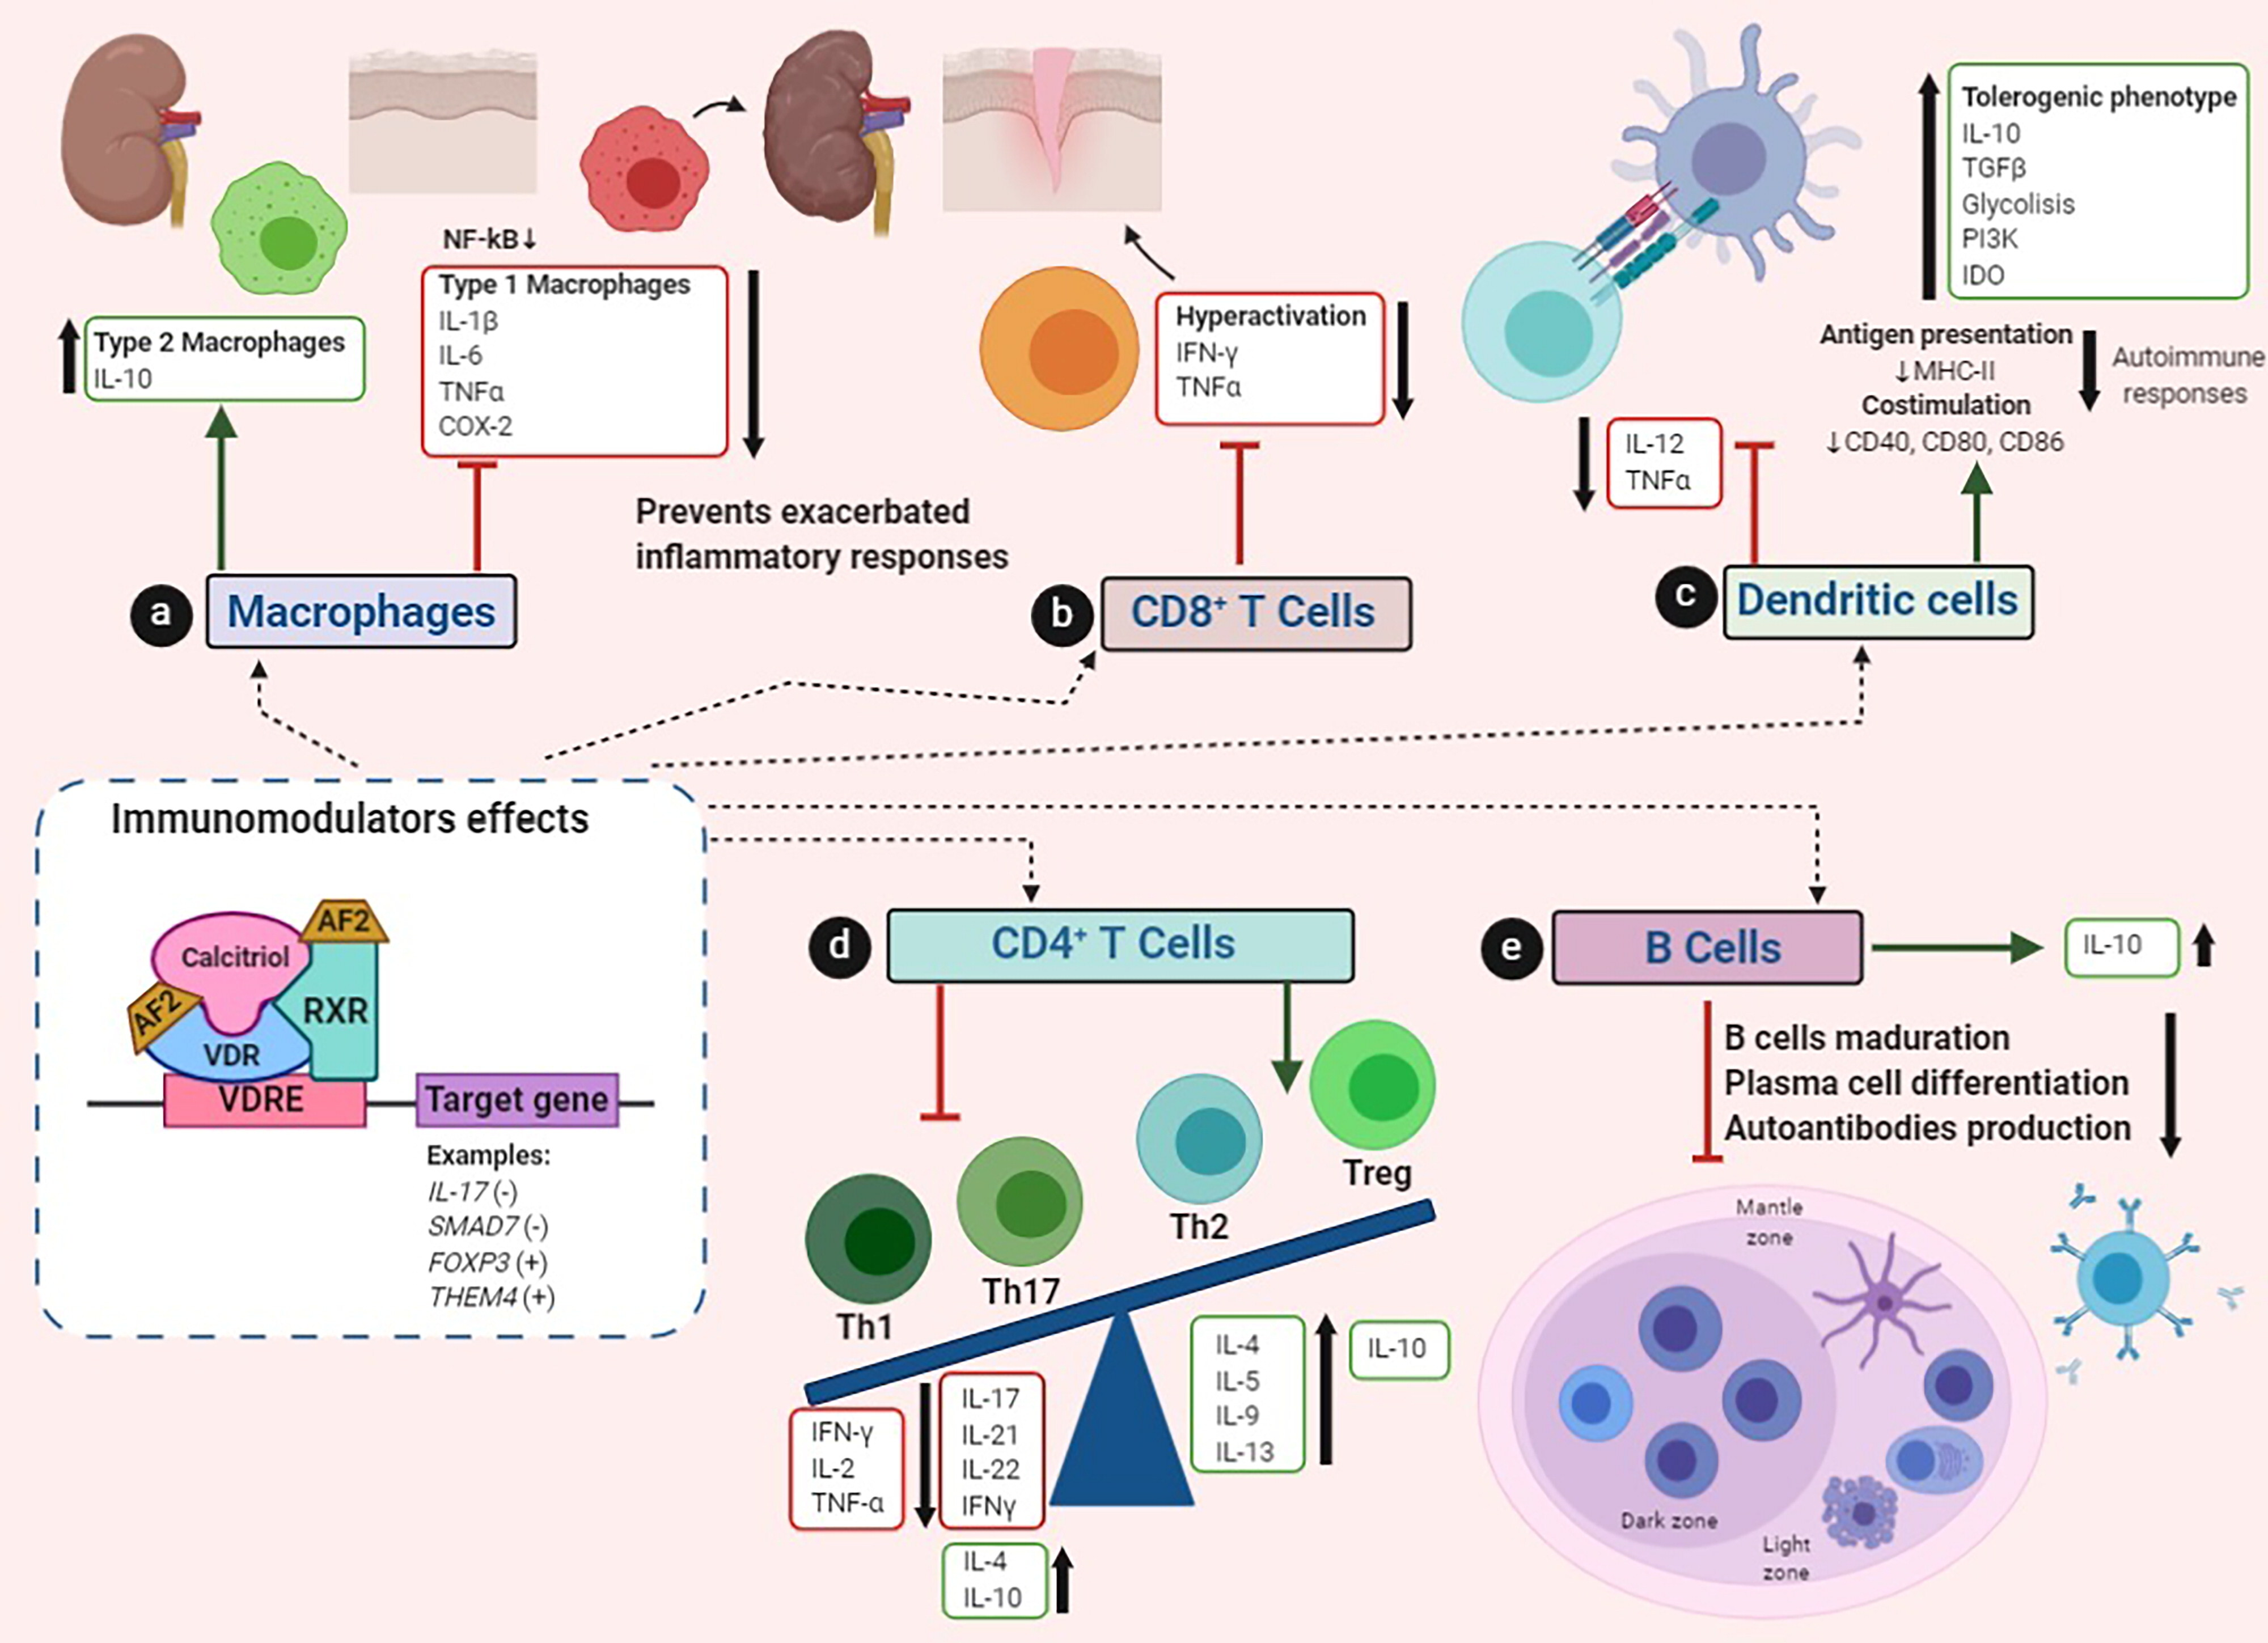
\includegraphics{figures/calcitriol-immunomodulatory.jpg}

}

\caption[Schéma récapitulatif des effets immunomodulateurs du
calcitriol.]{\label{fig-immunomod}\textbf{Schéma récapitulatif des
effets immunomodulateurs du calcitriol.} Le calcitriol se fixe sur le
\ac{VDR} qui en interagissant avec le \ac{VDRE} provoque une
transcription de gènes régulateurs de l'immunité, conduisant à des
effets globalement favorisant la suppression et tolérance immunitaire.
Cette modulation se manifeste directement par l'inhibition de facteurs
cytokines pro-inflammatoires et l'augmentation de cytokines
anti-inflammatoires ou indirectement en favorisant le phénotype de
cellules immunes immunosuppressives comme les macrophages de type M2,
les sous-types de lymphocytes \ac{Th2} et \ac{Treg} ou le phénotype
tolérogénique des cellules dendritiques \autocite{Meza-Meza.2022}.}

\end{figure}%

\section{Schéma d'une réponse antivirale
classique}\label{schuxe9ma-dune-ruxe9ponse-antivirale-classique}

La voie des interférons de type I (IFN-1) est centrale dans la réponse
antivirale initiale. Elle permet d'inhiber la réplication virale, de
protéger les cellules non-infectées et de stimuler l'immunité
lymphocytaire antivirale (lymphocytes T CD8, NK). Ces mécanismes
d'immunité innée conduisent à la lyse des cellules infectées et à
l'instauration d'une immunité durable. Dans l'ensemble, ces processus
éliminent le virus, limitent l'atteinte pulmonaire et mènent à une
potentielle guérison.

\section{Vitamine D et pouvoir
antiviral}\label{vitamine-d-et-pouvoir-antiviral}

\textcite{Bishop.2021}

Les études montrent globalement que la vitamine D augmente l'immunité
antivirale et en particulier par le biais de la réponse innée immune, et
inhibe les réponses cytokiniques pro-inflammatoires. La vitamine D
possède une implication dans la réponse immunitaire antivirale car de
nombreux virus respiratoires ciblent les cellules épithéliales
pulmonaires, qui sont très sensibles à la présence de vitamine D. Les
cellules épithéliales induisent fortement le \ac{CYP27B1} lors de
présence du calcidiol ainsi que lors de la détection d'ARN viraux double
brins \autocite{Bishop.2021}.

La réponse antivirale innée passe en partie par l'activation des
\acp{TLR}, qui cause l'induction du \ac{CYPB27B1} et du \ac{VDR}, médié
par l'activation du TLR2, induisant par la suite l'expression de
\emph{CAMP} \autocite{Liu.2006}. La vitamine D est ainsi un très fort
inducteur du gène \emph{CAMP} qui transcrit le peptide antimicrobien
cathélicidine LL-37 capable de se lier aux \ac{LPS} et de causer la
perméabilisation des membranes, et induit de CD14
\autocite{Hewison.2007}. Le CD14 est le cofacteur du TLR4 qui permet de
reconnaître classiquement le \ac{LPS.} Le calcitriol inhibe également le
signalement du facteur pro-inflammatoire \ac{nfkb} dans les cellules
pulmonaires \autocite{Bishop.2021}.

La vitamine D régule la production d'interférons et module la fonction
des cellules immunitaires antivirales ainsi qu'en induisant la
production de peptides antimicrobiens. En effet, elle stimule la
production des AMPs, \emph{CAMP}, \emph{HBD2}, \emph{DEFB4}, dont les
deux derniers éléments contiennent/permettent la génération du complexe
\ac{VDRE} \autocite{Bishop.2021}.

Les réponses transcriptionnelles initiales ayant lieu lors d'une
infection virale concernent en particulier les membres de la famille des
facteurs de régulation de l'interféron tels que IRF3 et IRF7, les
membres de la famille AP-1 et \ac{nfkb}. Le calcitriol agit en inhibant
le \ac{nfkb} qui est un puissant pro-inflammatoire, grâce à l'induction
de \ac{IKBa} \autocite{Bishop.2021}.

Un mécanisme clé de la réponse antivirale médiée par la vitamine D est
l'induction puissante de l'expression de \emph{CAMP} via le TLR2, gène
codant pour la forme active de la cathélicidine LL-37 qui va à son tour
favoriser la détection des ARN viraux double brins par le \ac{PRR} TLR3.
Le LL-37 peut se lier à l'ARN double brin viral qui se retrouve dans les
endosomes, où est situé le TLR3. Le TLR3 est un \ac{PRR} important dans
la reconnaissance du virus, et enclenche à son tour l'activation du
mécanisme immunitaire inné, en passant par le \ac{nfkb}. Les études
montrent également que le LL-37 possède une activité antivirale directe
qui perturbe les membranes virales \autocite{Bishop.2021}. Une étude
montre que lorsque la concentration de vitamine D est insuffisante, ou
lorsqu'un anticorps anti-LL37 est utilisé afin de bloquer l'effet de la
forme active de la cathélicidine, l'activité antivirale observé dans les
poumons est bloqué, et la supplémentation en vitamine D restaure le
pouvoir antiviral de LL-37 \autocite{Buonfiglio.2017}. Il est
intéressant de noter que cette induction de \emph{CAMP} dépend de la
concentration en calcidiol, et une concentration insuffisante ne permet
pas une induction en CAMP, ce qui renforce l'importance d'une
concentration adéquate en vitamine D appropriée pour le système
immunitaire \autocite{White.2022}.

Le calcitriol est capable d'induire NOD2 qui induit l'autophagie pour
augmenter la clairance virale. L'autophagie est un mécanisme clé dans le
contrôle de la réplication et l'infection virale, permettant la
dégradation des composants intracellulaires, y compris les protéines
virales et les acides nucléiques. En effet, le calcitriol induit
directement l'expression d'enzymes clés de l'autophagie comme Beclin1 et
PI3KC. en favorisant la cathélicidine qui induit Beclin1. Il peut
également favoriser indirectement l'autophagie en supprimant
l'inhibition de l'autophagie par la voie de signalisation mTOR, et en
stimulant le calcium intracellulaire et le \ac{NO} par le calcitriol
afin d'augmenter l'activité de PI3KC3 \autocite{Bishop.2021}.

\begin{figure}

\centering{

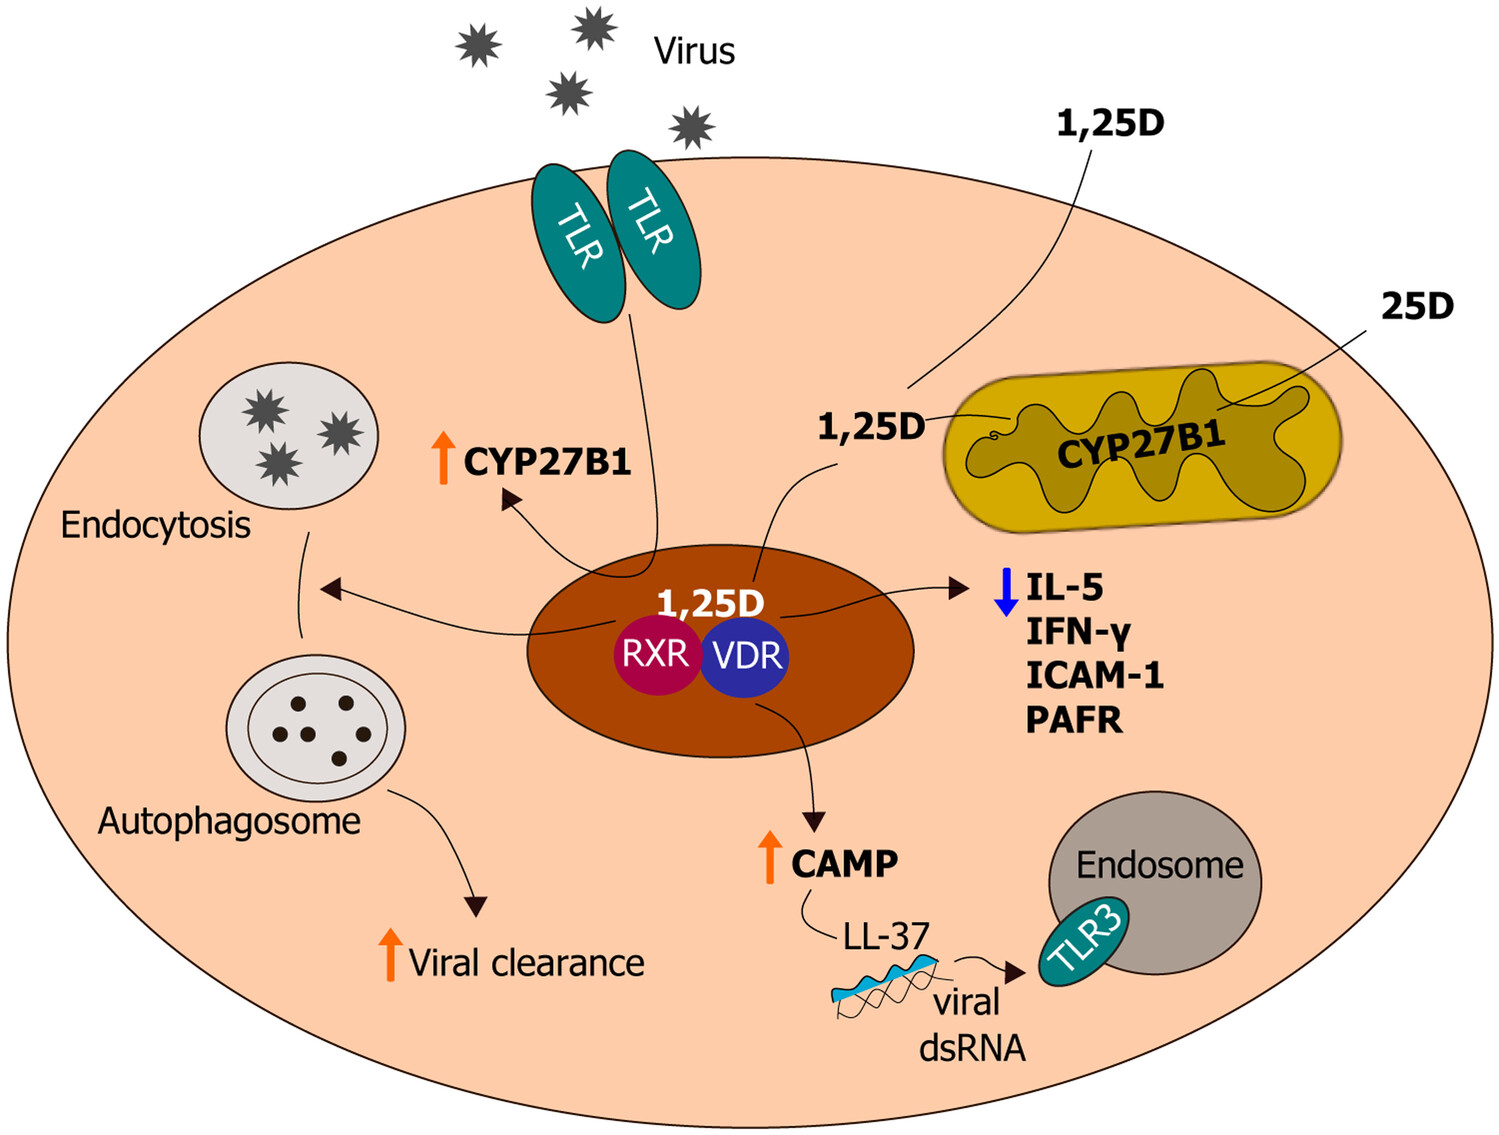
\includegraphics{figures/Ismailova.2022.-Antiviral_activity_of_vitamin_D_lung_cell.jpg}

}

\caption[Activité antivirale de la vitamine D dans une cellule
épithéliale pulmonaire.]{\label{fig-vd-antiviral}\textbf{Activité
antivirale de la vitamine D dans une cellule épithéliale pulmonaire.}
Illustration montrant les évènements qui sous-tendent le métabolisme et
la signalisation de la vitamine D au cours d'une infection virale et les
réponses induites par la 1,25D. Il s'agit notamment de l'induction de
l'expression du CAMP et de la suppression des cytokines inflammatoires
IL-5 et IFN-γ, ICAM-1 et PAFR par l'intermédiaire de la 1,25D. La forme
mature de CAMP, LL37, se lie à l'ARNdb viral, ce qui permet une liaison
efficace au TLR3 endosomal, augmentant la signalisation du TLR3 et la
clairance virale subséquente. Un autre mécanisme d'élimination virale
est l'induction de l'autophagie par le 1,25D \autocite{Ismailova.2022}.}

\end{figure}%

\section{Metabolisme de la vitamine D dans le système immunitaire
inné}\label{metabolisme-de-la-vitamine-d-dans-le-systuxe8me-immunitaire-innuxe9}

Les cellules immunitaires contrôlent leur propre expression du \ac{VDR}
et du \ac{CYP27B1} afin de moduler les effets du calcitriol sur leur
activation, en fonction des signaux et du statut inflammatoire de
l'environnement. En effet, la \ac{CYP27B1} et le \ac{VDR} peuvent être
induites par les monocytes et macrophages en réponse au signalement des
\ac{PRR} tel que l'activation de CD14-TLR4 (CD14 étant le corécepteur de
TLR4 et une cible d'induction du calcitriol) \autocite{Stoffels.2009},
la stimulation de TLR1 et TLR2 \autocite{Liu.2006}.

Certaines cytokines sont également capables de réguler l'expression de
\ac{CYP27B1} tel que l'\ac{ifng} \autocite{Stoffels.2009} et l'IL-15 en
tant qu'intermédiaire après stimulation du TLR1/2
\autocite{Krutzik.2008}.

L'expression de \ac{CYP27B1} et de \ac{VDR} contribue à la synthèse de
calcitriol grâce au calcidiol circulant, et contribue au fonctionnement
du mécanisme immunitaire.

\newpage{}

\chapter{Vitamine D et COVID-19}\label{vitamine-d-et-covid-19}

\section{Physiopathologie de la COVID-19 concernant le système
immunitaire}\label{physiopathologie-de-la-covid-19-concernant-le-systuxe8me-immunitaire}

\begin{itemize}
\item
  La \ac{COVID-19} est causée par le virus \ac{SARS-CoV-2} qui est un
  virus à ARN simple brin enveloppé qui appartient à la famille des
  Coronaviridae. Le virus envahit l'organisme par le biais de la
  protéine de pointe appelée spike protein (S). La protéine de pointe
  est impliquée dans la liaison aux récepteurs de surface des cellules
  hôtes, notamment l'\ac{ACE2}, qui est notamment impliquée dans le
  \ac{SRAA}.
\item
  Lorsque la réponse inflammatoire innée et adaptative ne devient plus
  protectrice mais devient exacerbée, associée à une réplication virale
  non controllée et des cellules infectée non éliminée, la réponse
  immunitaire se perpétue et s'aggrave, entraînant un \ac{SDRA} ou une
  \ac{CIVD} \autocite{Contreras-Bolívar.2023}.
\end{itemize}

\subsection{Processus d'infection : entrée dans les cellules hôtes,
réplication
virale}\label{processus-dinfection-entruxe9e-dans-les-cellules-huxf4tes-ruxe9plication-virale}

Le \ac{SARS-CoV-2} utilise sa protéine de pointe pour se fixer à la
surface des cellules respiratoires humaines. Une fois attaché à
\ac{ACE2}, le virus fusionne avec la membrane cellulaire, permettant
ainsi son entrée dans la cellule. Une fois à l'intérieur de la cellule,
le génome viral est libéré, et le virus commence à se répliquer en
utilisant les ressources de la cellule hôte. La réplication virale
aboutit à la production de nombreuses particules virales qui peuvent
infecter d'autres cellules, propageant ainsi l'infection dans le tissu
pulmonaire et au-delà.

Après fusion des membranes virales et cellulaires, le SARS-CoV-2 pénètre
et infecte les cellules épithéliales et les pneumocytes de type II. La
liaison de la protéine S virale avec l'\ac{ACE2} entraîne la sécrétion
de cytokines (TNF-α, IL-1, IL-6, chimiokines), ce qui provoque une
hyperperméabilité́ capillaire ainsi que l'attraction d'\ac{IFN-1} et de
cellules inflammatoires.

L'infection par le SARS-CoV-2 downrégule l'activité ACE2 ce qui cause
une accumulation de Ang II qui peut causer des conséquences de la
suractivation du SRAA (\Cref{fig-sraa-covid19}) \autocite{Mahdavi.2020}.

\subsection{Réponse immunitaire innée et adaptative face à
l'infection}\label{ruxe9ponse-immunitaire-innuxe9e-et-adaptative-face-uxe0-linfection}

Lorsque le SARS-CoV-2 infecte les cellules respiratoires, il déclenche
une série de réponses immunitaires impliquant d'abord des cellules
immunitaires innées telles que les macrophages et les cellules
dendritiques qui détectent la présence du virus. La réponse innée
entraîne la production de cytokines pro-inflammatoires pour attirer
davantage de cellules immunitaires sur le site de l'infection par le
biais de chimiokines tel que l'\ac{IL-8} et le MCP-1 qui attirent les
neutrophiles, granulocytes et monocytes.

Simultanément, le système immunitaire adaptatif est mobilisé. Les
lymphocytes T cytotoxiques (CD8\textsuperscript{+}) identifient et
détruisent les cellules infectées par le virus, limitant ainsi la
propagation du \ac{SARS-CoV-2}. Les lymphocytes B produisent des
anticorps spécifiques qui peuvent neutraliser le virus. Ensemble, ces
deux composantes de la réponse immunitaire contribuent à contrôler
l'infection.

\begin{itemize}
\tightlist
\item
  Rôle de IL-17 dans la physiopathologie du COVID-19 : IL-17 est
  impliqué dans des risques de thrombose et de \ac{SDRA}
  \autocite{Pal.2022}.
\item
  La dysrégulation de ACE2 impliqué dans le SRAA peut causer une tempête
  cytokinique et d'autres réponses inflammatoires pathogéniques, pouvant
  mener à une défaillance d'organe multiviscérale
  \autocite{Argano.2023}.
\end{itemize}

\subsection{Tempête cytokinique}\label{tempuxeate-cytokinique}

\begin{itemize}
\tightlist
\item
  Lorsque la réponse immunitaire est excessive, elle peut entraîner une
  tempête de cytokines, également appelée orage cytokinique, qui est
  caractérisée par une libération massive de cytokines
  pro-inflammatoires.
\item
  COVID-19+ et soins intensifs : Plus de IL-2, IL-7, IL-10, G-CSF,
  \ac{ifng}, MCP et \ac{tnfa} que les patients non soins intensifs.
\item
  Niveaux d'IL-6 plus élevés chez les patients COVID-19 sévères que
  modéré et léger.
\item
  Présence de lymphocyte Th1 et Th2 suractivé lors de la tempête
  cytokinique avec patients COVID-19 et potentiellement une dysfonction
  immunitaire sévère, et activation monocytaire.
\item
  Immunosuppression des CD4+, CD8+, NK.
\end{itemize}

La tempête cytokinique peut endommager les poumons et causer une
infiltration pulmonaire et une sévère hypoxie, résultant en une
dysfonction de la respiration. Elle est également impliquée lors des
défaillances d'organes multiviscérales \autocite{Argano.2023}.

\subsection{Sepsis}\label{sepsis}

Le sepsis est une complication grave de l'infection par le
\ac{SARS-CoV-2} qui peut entraîner une défaillance multi-organique et la
mort. Le sepsis est caractérisé par une réponse inflammatoire systémique
incontrôlée qui peut entraîner des dommages aux organes vitaux tels que
les poumons, le cœur, le foie et les reins.

Traditionnellement l'activation immune est considérée comme étant le
stage précoce de l'inflammation, et l'immunosuppression la phase tardive
de l'inflammation après élimination du pathogène, mais des études
récentes ont montré que l'activation immune et l'immunosuppression
coexistes tout au long de la réponse immune et que les processus
inflammatoires résultent d'une balance immune entre ces deux processus.
Le sepsis est de ce fait le résultat d'une hyperinflammation incontrôlée
et d'une immunosuppression insuffisante. Lors du sepsis, la vitamine D a
un rôle inhibiteur des cytokines pro-inflammatoires (IL-12, \ac{ifng},
IL-6, IL-8, \ac{tnfa}, IL-17, IL-9), d'inhibition de la transcription du
COX-2 et de la prolifération, différenciation, activation et production
d'immunoglobuline des lymphocytes B et induit l'apoptose des lymphocytes
B. En contrepartie la vitamine D promeut la production de cytokines
anti-inflammatoires (IL-4, IL-5, IL-10) et la différenciation des
lymphocytes T régulateurs, des monocytes et des cellules dendritiques à
phénotype tolérogènes, et est un fort inducteur de la cathélicidine
hCAP18, précurseur du LL-37 qui a des propriétés anti-infectieuses et en
particulier dans la COVID-19 en empêchant l'entrée du virus dans la
cellule en se liant à la protéine Spike.
\autocite{Cutuli.2024,Keutmann.2022,Ødum.2023}

\section{Rationnel du mécanisme physiologique de l'usage de la vitamine
D dans la
COVID-19}\label{rationnel-du-muxe9canisme-physiologique-de-lusage-de-la-vitamine-d-dans-la-covid-19}

\textcite{Borsche.2021}: La vitamine D agit sur deux principaux
évènements mettant le pronostic vital en jeu dans la physiopathologie de
la COVID-19: \ac{SDRA} et \ac{CRS}, par un mécanisme particulier
spécifique entre la vitamine D et le SARS-CoV-2 :

\begin{itemize}
\tightlist
\item
  la vitamine D agit comme modulateur du \ac{SRAA} en diminuant la
  rénine et en augmentant ACE2
\item
  La diminution de l'angiotensine II (ATII) et l'augmentation de
  Ang(1-7) ce qui favorise la voie MasR.
\end{itemize}

Selon \textcite{Borsche.2021}, il existe 5 mécanismes par lesquels la
vitamine D supporte le système immunitaire :

\begin{itemize}
\tightlist
\item
  Diminution de production de Th1
\item
  Diminution du \ac{CRS}
\item
  Induction de la production de LL-37 (cathélicidine), peptide
  antimicrobien
\item
  Modulation de la fonction endothéliale et de la perméabilité
  vasculaire
\item
  Réduction des anomalies de la coagulabilité dans les patients COVID-19
\end{itemize}

Selon \textcite{Pal.2022} : 3 mécanismes supportant l'action de la
vitamine D

\begin{itemize}
\tightlist
\item
  Induction de LL-37 et de sa protection antivirale ; note sur la
  relation inverse entre LL-37 et IL-17, uprégulé lors du COVID-19.
\item
  Diminution de la production de cytokines pro-inflammatoires
  (\ac{IL-6}, \ac{tnfa}, augmentation \ac{IL-10})
\item
  Action sur le \ac{SRAA}
\end{itemize}

\subsection{Système Rénine Angiotensine
Aldostérone}\label{systuxe8me-ruxe9nine-angiotensine-aldostuxe9rone}

\begin{itemize}
\item
  La physiopathologie de la COVID-19 implique le \ac{SRAA} causé par
  l'entrée du virus dans les cellules ce qui provoque l'endocytose du
  récepteur-enzyme ACE2 et inhibant ainsi ses fonctions. ACE2 est une
  enzyme importante dans le \ac{SRAA}, qui possède un effet antagoniste
  du récepteur ACE, les deux agissant comme une balance afin de réguler
  diverses fonctions physiologiques telles que la pression artérielle,
  l'inflammation, la fibrose, la prolifération cellulaire, la
  régénération tissulaire, et la réponse immunitaire
  (\Cref{fig-ace2-masR}) \autocite{Brojakowska.2020}.
\item
  Il a été observé que le calcitriol diminue le ratio ACE/ACE2,
  diminuant la uprégulation de ACE et la downrégulation de ACE2 dans
  chez les rats diabétiques, réprime le récepteur AT1 de l'Ang II et
  ACE, et réduit la formation de Ang II, tout en augmentant l'expression
  des éléments ACE2, Ang(1-7), MasR \autocite{Mahdavi.2020}.
\item
  De plus, ACE2 n'est pas seulement le récepteur d'entrée du SARS-CoV-2
  mais joue également un rôle dans la régulation immune en agissant par
  d'autres mécanismes indirects \autocites[ ]{Argano.2023}{Zipeto.2020},
  tel que l'interaction avec les protéines ADAM17 et TMPRSS2 qui
  modulent des cytokines pro-inflammatoires.
\item
  De plus, la bradykinine, régulée par ACE, est impliquée dans les
  processus perturbés par la COVID-19. ACE est responsable de la
  dégradation de la bradykinine, qui est impliquée dans le système
  bradykinine, régulant la pression artérielle, induisant la
  vasodilatation, natriurèse et hypotension (\Cref{fig-ace2-masR}). La
  bradykinine serait également impliqué lors de l'inflammation car elle
  induit le recrutement des neutrophiles et une augmentation de la
  perméabilité vasculaire. L'analyse computationnelle de l'expression
  des gènes des fluides de lavages bronchoalvéolaires de
  \textcite{Garvin.2020} révèle une ``tempête bradykinique'', où
  l'expression de bradykinine chez les patients COVID-19 est en
  surreprésentation par rapport aux patients contrôles. De plus,
  l'expression de ACE2 est également surreprésentée chez les patients
  COVID-19, ce qui implique une régulation négative de ACE par ACE2,
  conduisant à une augmentation de la bradykinine. L'augmentation de
  bradykinine induit une vasodilatation et une perméabilité vasculaire.
  La tempête bradykinique explique la plupart de la symptomatologie de
  la COVID-19 \autocite{Garvin.2020}.
\end{itemize}

\begin{figure}

\centering{

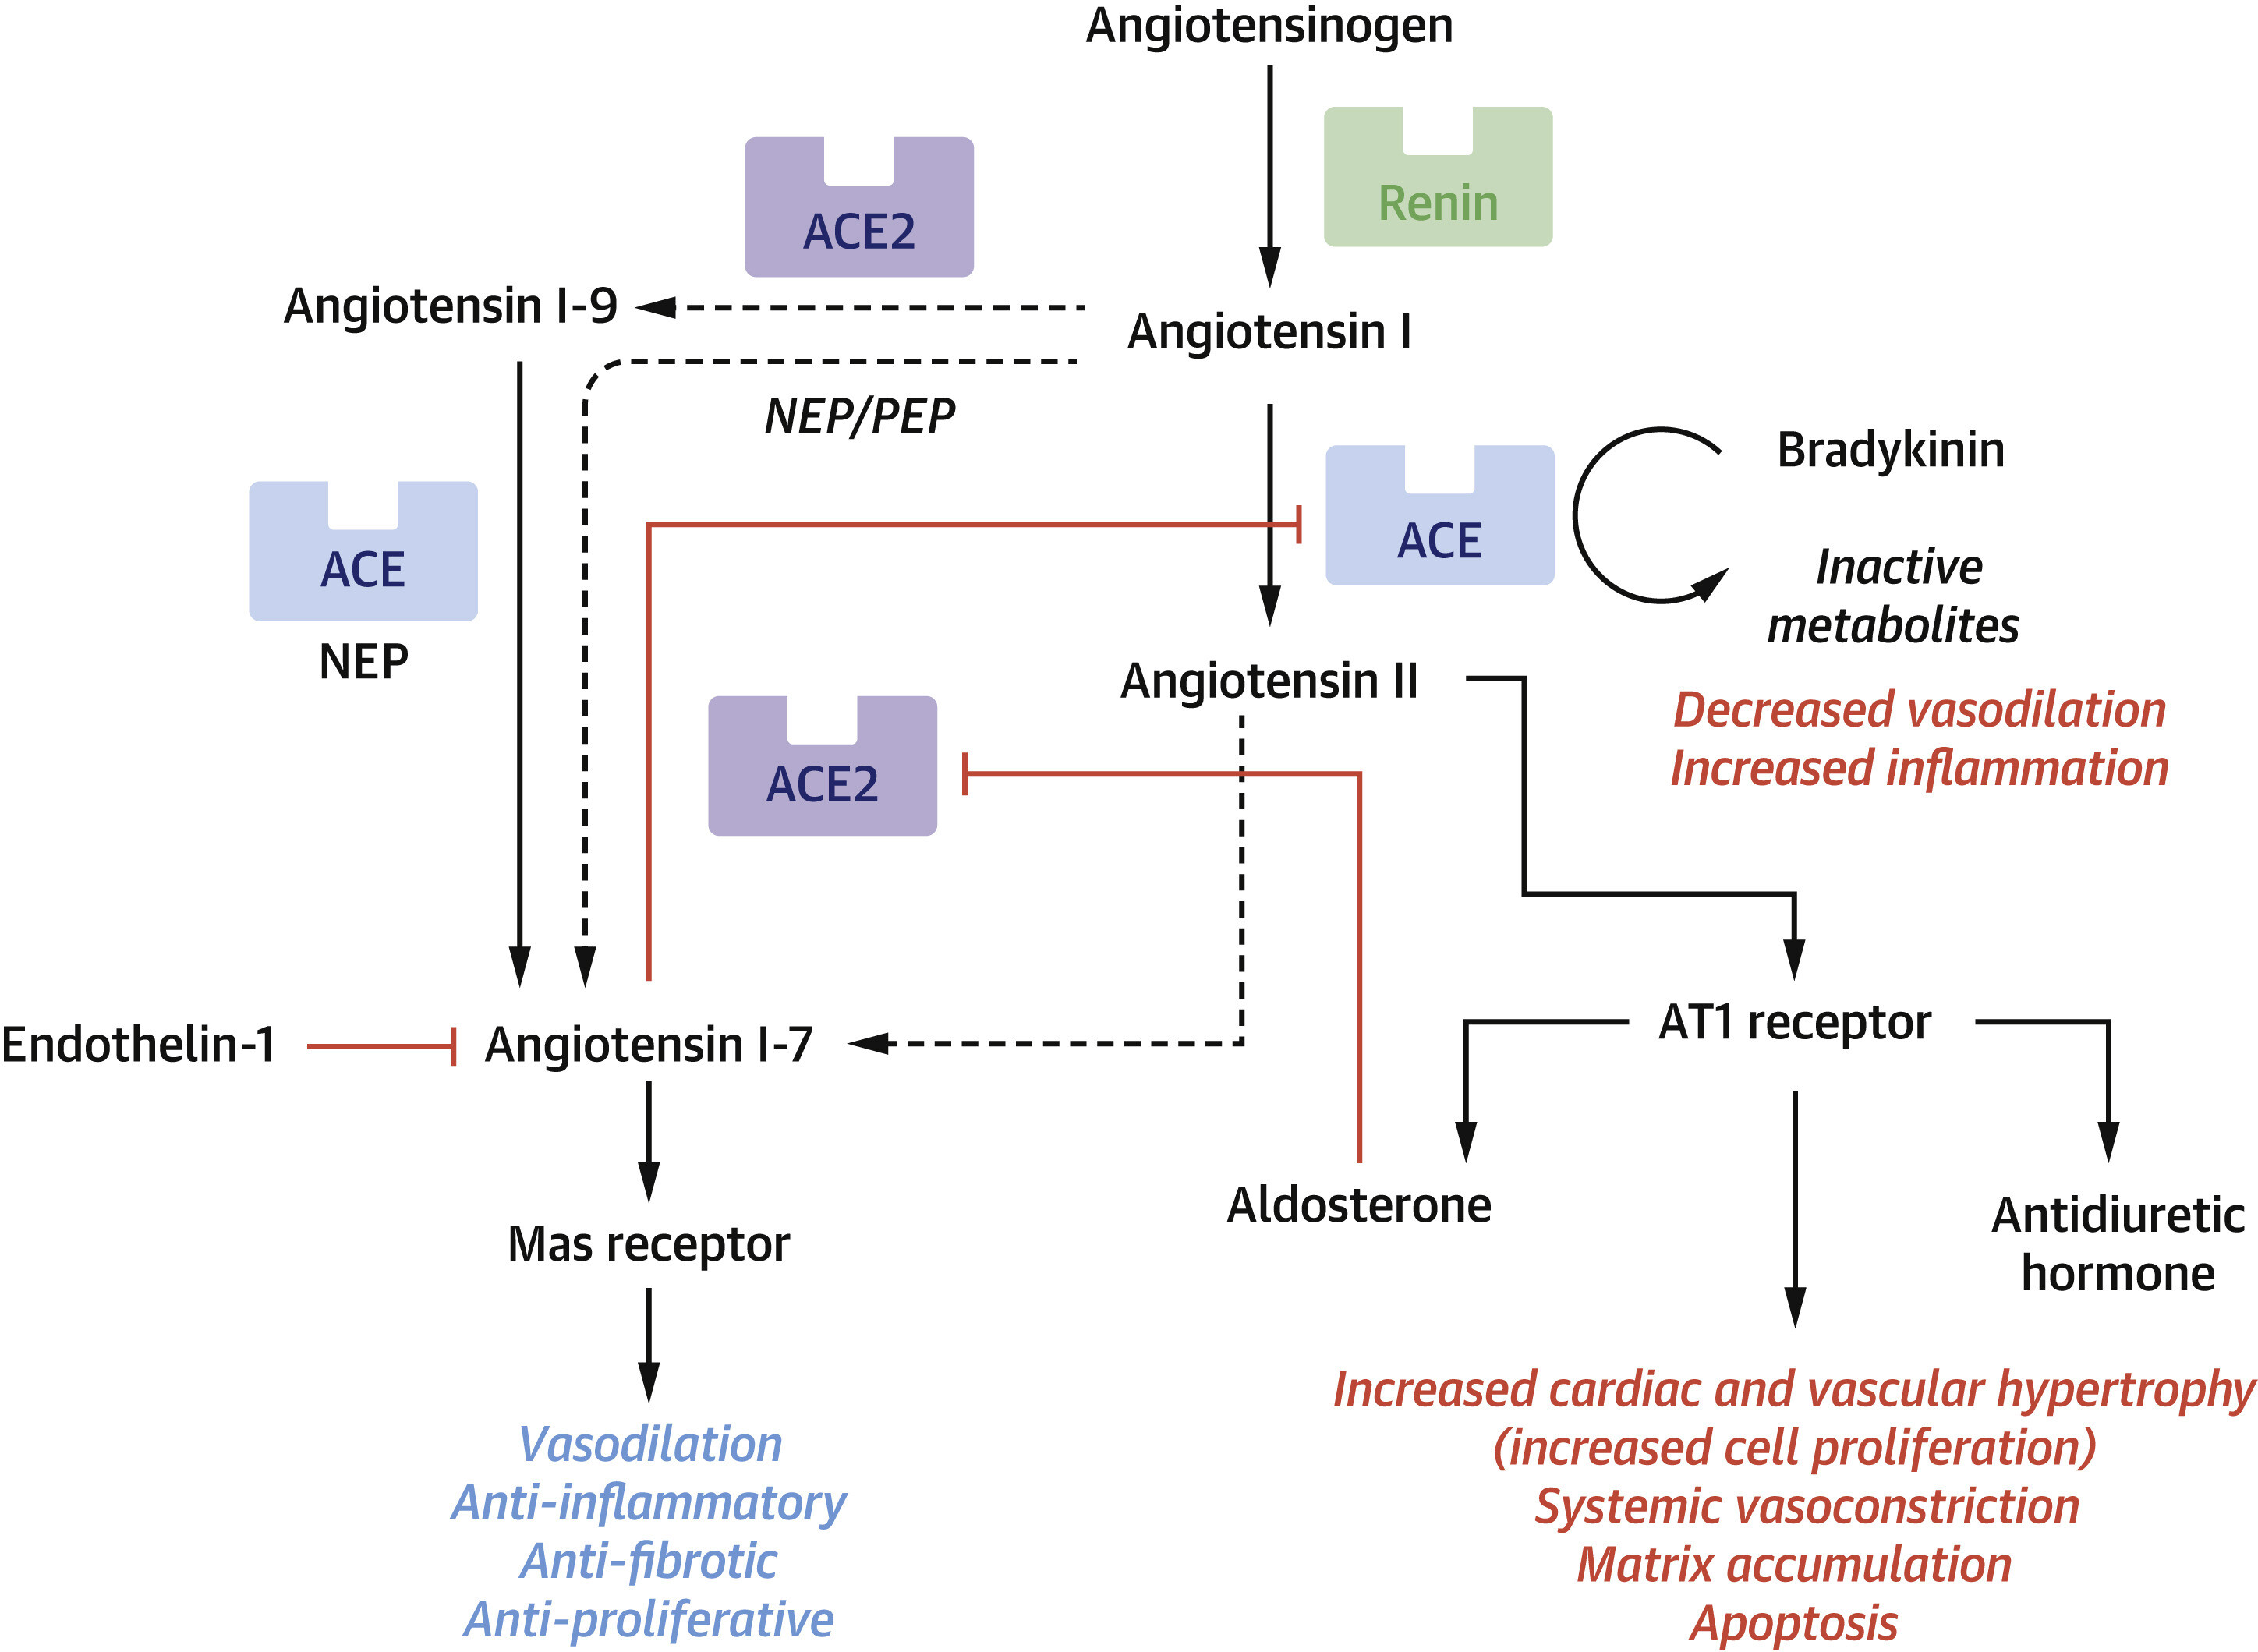
\includegraphics{figures/Brojakowska-RAS-ACE2-Regulation.jpg}

}

\caption[Régulation du SRAA et de l'axe
ACE2/Ang-1-7/AT1/MasR]{\label{fig-ace2-masR}\textbf{Régulation du SRAA
et de l'axe ACE2/Ang-1-7/MasR \autocite{Brojakowska.2020}.}}

\end{figure}%

\begin{figure}

\centering{

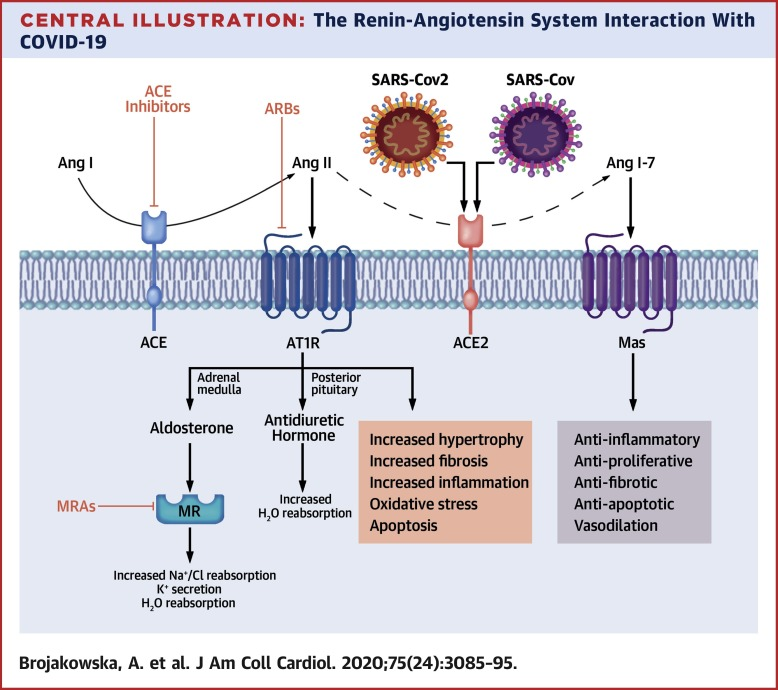
\includegraphics{figures/Brojakowska-RAS-COVID-19.jpg}

}

\caption[Interaction du SRAA avec la
COVID-19.]{\label{fig-sraa-covid19}\textbf{Interaction du SRAA avec la
COVID-19 \autocite{Brojakowska.2020}.}}

\end{figure}%

\begin{itemize}
\tightlist
\item
  \textcite{Li.2002} ont établi une relation entre la rénine et le
  système rénine-angiotensine-aldostérone. La vitamine
  D\textsubscript{3} a été observée comme étant un régulateur négatif du
  \ac{SRAA}. Lorsque le VDR est KO, l'activité du SRAA est augmentée.
  L'ajout de vitamine D diminue la production de rénine.
\end{itemize}

\begin{figure}

\centering{

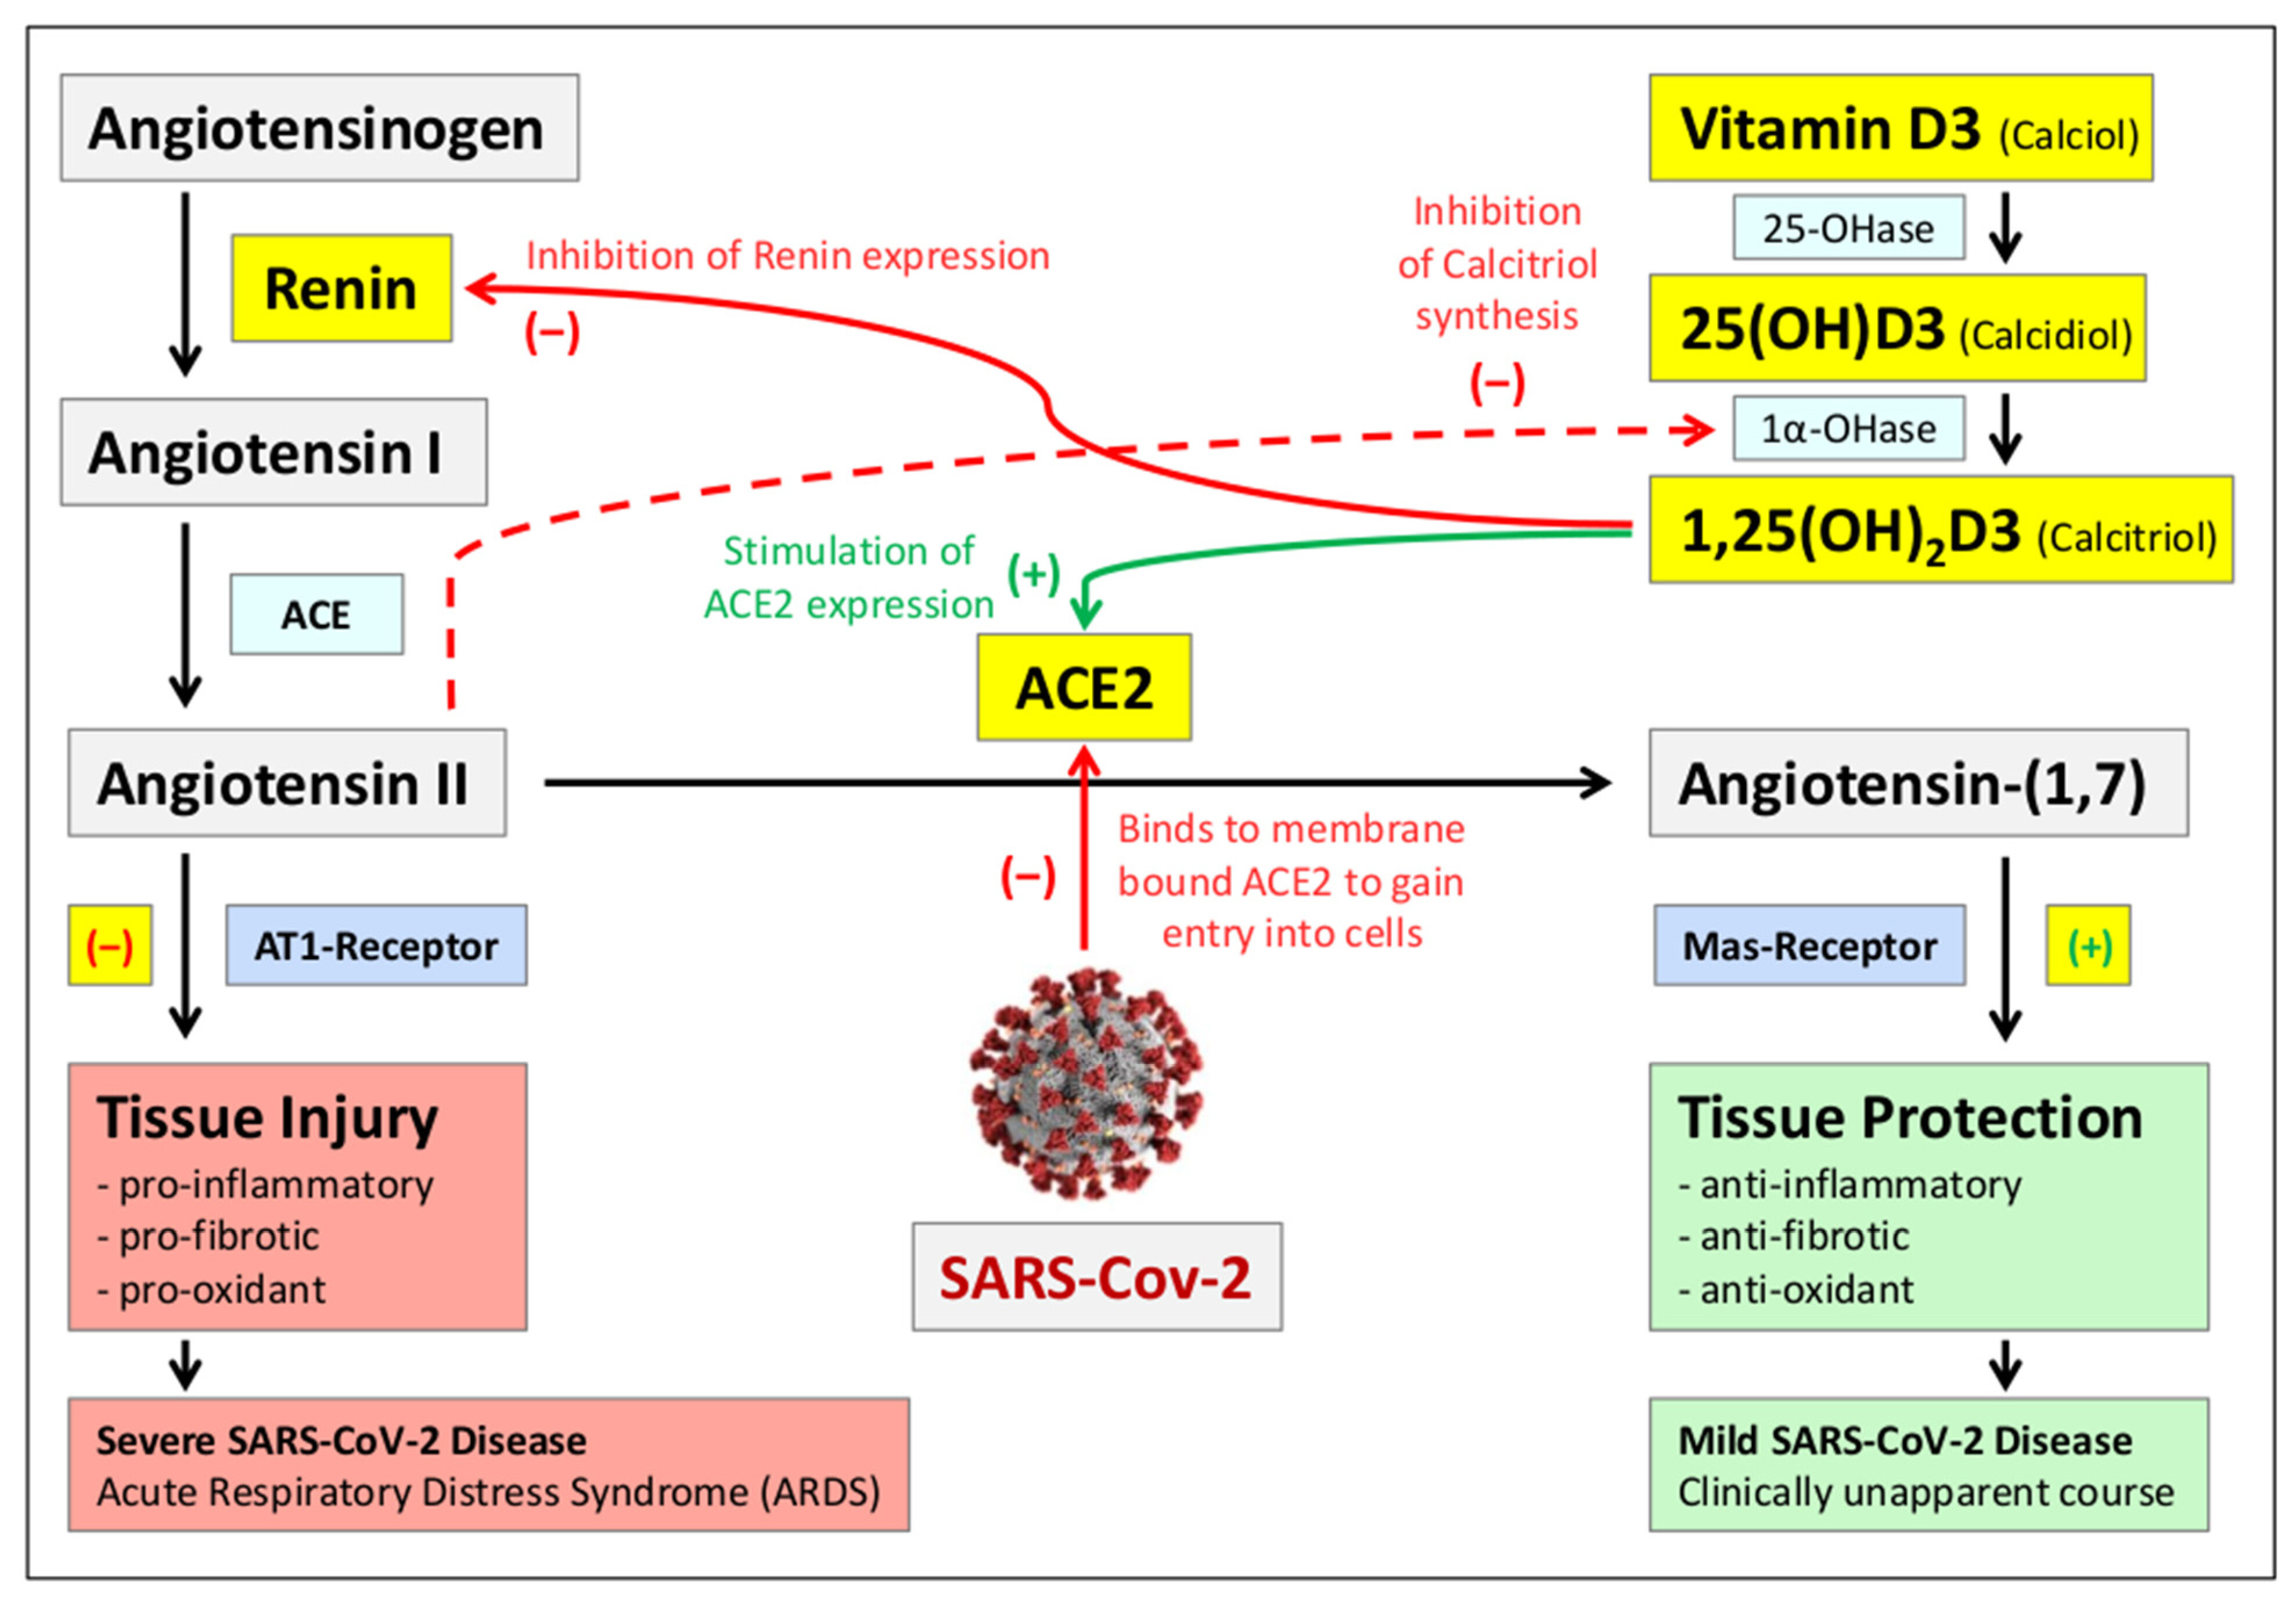
\includegraphics{figures/borsche.2021-vd-ras.jpg}

}

\caption[Schéma du rôle du la vitamine D dans l'inhibition du
SRAA.]{\label{fig-vd-ras}\textbf{Schéma du rôle du la vitamine D dans
l'inhibition du SRAA \autocite{Borsche.2021}.}}

\end{figure}%

\subsection{Mécanisme lié l'inhibition de
l'hyperinflammation}\label{muxe9canisme-liuxe9-linhibition-de-lhyperinflammation}

SARS-CoV-2, cause des dégâts notamment par une inflammation incontrôlée
médiée notamment par l'activation du SRAA, qui peut jouer un rôle
exacerbant l'inflammation et une tempête cytokinique.

\subsubsection{Mécanisme impliquant l'immunité
innée}\label{muxe9canisme-impliquant-limmunituxe9-innuxe9e}

\begin{itemize}
\item
  Le calcitriol, par l'induction de LL-37, peut réduire la NETose des
  neutrophiles et inhiber la liaison entre le SARS-CoV-2 et ACE2. Le
  calcitriol peut atténuer le TLR2 qui reconnaît le SARS-CoV-2 et
  engendre une cascade inflammatoire, inhiber la voie subséquente de
  \ac{nfkb} et l'inflammasome NLRP3. Le calcitriol favorise l'autophagie
  par le biais de LL-37, qui est un mécanisme de défense contre les
  infections virales et peut inhiber la réplication virale
  \autocite{Gotelli.2022}.
\item
  De plus, LL-37 est inversement corrélé aux niveaux de IL-17, qui est
  impliqué dans des risques de thrombose et de \ac{SDRA}
  \autocite{Pal.2022}.
\item
  Action potentielle par le biais du DBP recrutant des neutrophiles et
  activant le complément C5a, induisant une inflammation systémique ; la
  présence de vitamine D entre en compétition avec le DBP sur le même
  site de liaison d'activation du complément et réduit l'action du DBP
  \autocite{Speeckaert.2020,Contreras-Bolívar.2023}.
\end{itemize}

\subsubsection{Mécanisme impliquant l'immunité
adaptative}\label{muxe9canisme-impliquant-limmunituxe9-adaptative}

\begin{itemize}
\tightlist
\item
  Le calcitriol diminue les cytokines IL-12 et IL-23 qui promeut un
  phénotype tolérogène des cellules dendritiques
  \autocite{Gotelli.2022}.
\item
  Le calcitriol favorise la différenciation des lymphocytes B vers des
  plasmocytes sécréteurs d'IgA \autocites[ ]{Gotelli.2022}{Chauss.2022}
\end{itemize}

Une étude menée par \textcite{Chauss.2022} examine les mécanismes
moléculaires qui conduisent à la rétractation et à l'arrêt du phénotype
\ac{Th1}. Les analyses issues du single cell RNA-sequencing ont permises
de mettre en évidence que le complément induisait l'expression de
\ac{VDR} et de \ac{CYP27B1}, permettant aux cellules d'utiliser la
vitamine D. La vitamine D permet ainsi de faire passer le phénotype
pro-inflammatoire \ac{Th1} au phénotype anti-inflammatoire
IL-10\textsuperscript{+}. La vitamine D active plusieurs facteurs de
transcriptions tels que c-JUN, STAT3 et BACH2 qui contribuent au rôle de
répression des \ac{Th1} et Th17 et induisent l'IL-10 par le biais du
signalement de STAT3. De plus, les patients présentaient des cellules
CD4+ à prédominance \ac{Th1} et montrent une dérépression de gènes
normalement downrégulés par la vitamine D. - Il est intéressant de noter
la vitamine D a permise d'induire l'IL-6, qui possède dans ce cas un
rôle immunomodulateur contrairement au rôle standard de pro-inflammation
\autocite{Chauss.2022}.

\subsection{Mécanisme antiviral induit par la vitamine D contre la
COVID-19}\label{muxe9canisme-antiviral-induit-par-la-vitamine-d-contre-la-covid-19}

En interagissant avec le \ac{VDR} qui se trouve sur les cellules
immunitaires (cellules B, cellules T et cellules présentatrices
d'antigènes) et les cellules épithéliales pulmonaires, le complexe
calcitriol - \ac{VDR} se lie sur le \ac{VDRE}. Le \ac{VDRE} est situé
sur le promoteur du gène \emph{CAMP}. La vitamine D stimule l'expression
de ce gène, et induit la cathélicidine humaine hCAP-18, précurseur de
LL-37, clivé par la protéinase 3 en LL-37. Le domaine C-terminal de
hCAP18 nommé LL-37, est un peptide antimicrobien qui a un rôle dans
l'immunité innée et adaptative, et a un rôle antiviral contre le
SARS-CoV-2. En effet, le LL-37 se lie avec une grande affinité à la
protéine de pointe S du SARS-CoV-2, empêchant celle-ci de se lier à la
cellule hôte. Le LL-37 se lie également à ACE2 et empêche la protéine de
pointe de se lier et donc d'entrer dans la cellule hôte. Des niveaux
sériques plus faibles de LL-37 sont associés à la gravité de la maladie
et à la durée du séjour à l'hôpital \autocites[ ]{Keutmann.2022}[
]{Cutuli.2024}{Shiravi.2022,Munshi.2021}.

La vitamine D possède des effets antioxydantes en modulant l'activité
mitochondriale, la uprégulation du glutathion, de la peroxydase et
superoxyde dismutase, et en downrégulant la NADPH oxydase. La présence
de NO et de superoxyde peut exercer une activité antivirale \autocites[
]{Shiravi.2022}{Contreras-Bolívar.2023}.

\begin{figure}

\centering{

\includegraphics{figures/Contreras-Bolívar.2023-vd_paracrine_intracrine_functions.jpg}

}

\caption[Représentation schématique des fonctions paracrines et
intracrines de la vitamine D et de ses métabolites et actions dans les
systèmes immunitaires innés et
adaptatifs.]{\label{fig-vd-covid-function}\textbf{Représentation
schématique des fonctions paracrines et intracrines de la vitamine D et
de ses métabolites et actions dans les systèmes immunitaires innés et
adaptatifs.} A : Synthèse de la vitamine D. B1 : Immunité adaptative. B2
: immunité innée. C : Réponse inflammatoire médiée par le SARS-CoV-2
\autocite{Contreras-Bolívar.2023}.}

\end{figure}%

La \ac{COVID-19} est caractérisée souvent par une hyperinflammation non
résolue, associée à une infection aiguë des poumons. De plus, la
majorité des personnes sont déficientes en vitamine D
(Section~\ref{sec-statut-vd}). La vitamine D montre donc son potentiel
dans cadre de la \ac{COVID-19} en renforçant le système immunitaire
contre l'infection virale pulmonaire, tout en permettant au système
immunitaire de pouvoir basculer du programme d'hyperinflammation vers un
équilibre immunitaire plus tolérogène.

\subsection{Vitamine D et
neuroprotection}\label{vitamine-d-et-neuroprotection}

\textcite{Shiravi.2022} rapporte que ACE2 est présent dans les neurones
et astrocytes. L'interaction avec ACE2 dans l'endothélium capillaire
peut endommager la barrière hémato-encéphalique. La vitamine D peut
avoir un effet neuroprotecteur car le VDR est également trouvé dans les
neurones et astrocytes ainsi que la présence de 1-alpha hydroxylase. Les
études \emph{in vitro} montrent que la vitamine D possède un pouvoir
anti-inflammatoire sur les microglies en diminuant la production de
IL-6, \ac{tnfa}, et NO, ainsi que des pouvoir neuroprotecteurs en
inhibant la iNOS qui produit du NO qui endommage les cellules. De plus,
la vitamine D possède un pouvoir anti-oxydant en régulant l'enzyme
impliquée dans le cycle du glutathion.

\section{Statut en vitamine D, épidémiologie du risque infectieux en
général et COVID-19 en particulier}\label{sec-statut-vd}

\begin{itemize}
\tightlist
\item
  La majorité de la population possède un statut en vitamine D même
  insuffisant pour des effets bénéfiques à visée osseuse (inférieur à 20
  ng/mL). De plus, les personnes âgées supérieurs à 70 ans qui sont à
  plus fort risque de symptômes sévères sont souvent déficitaires en
  vitamine D comparés aux personnes plus jeunes.
\item
  Des études ont rapportés que les pays de l'hémisphère sud avaient un
  taux de mortalité plus bas que les pays de l'hémisphère nord, tel que
  les Etats-Unis (68 par million) contre l'Australie (2 par millions).
  Il existe des exceptions tels que l'Espagne et l'Italie qui ont une
  plus grande mortalité, associé à une prévalence de déficience en
  vitamine D plus importante, qui peuvent s'expliquer par le biais de la
  préférence à l'ombre, et de la pigmentation plus importante de la peau
  qui diminue la synthèse en vitamine D. Les pays scandinaves ont une
  mortalité plus basse, associé à une consommation plus fréquente
  d'huile de foie de morue ainsi que de fortifications de laits et de
  laitages. La mortalité due au COVID-19 est associé à des comorbidités
  telles que l'âge et des maladies chroniques, qui sont également
  associés à une concentration plus basse de vitamine D
  \autocite{Bishop.2021}.
\end{itemize}

\begin{figure}

\centering{

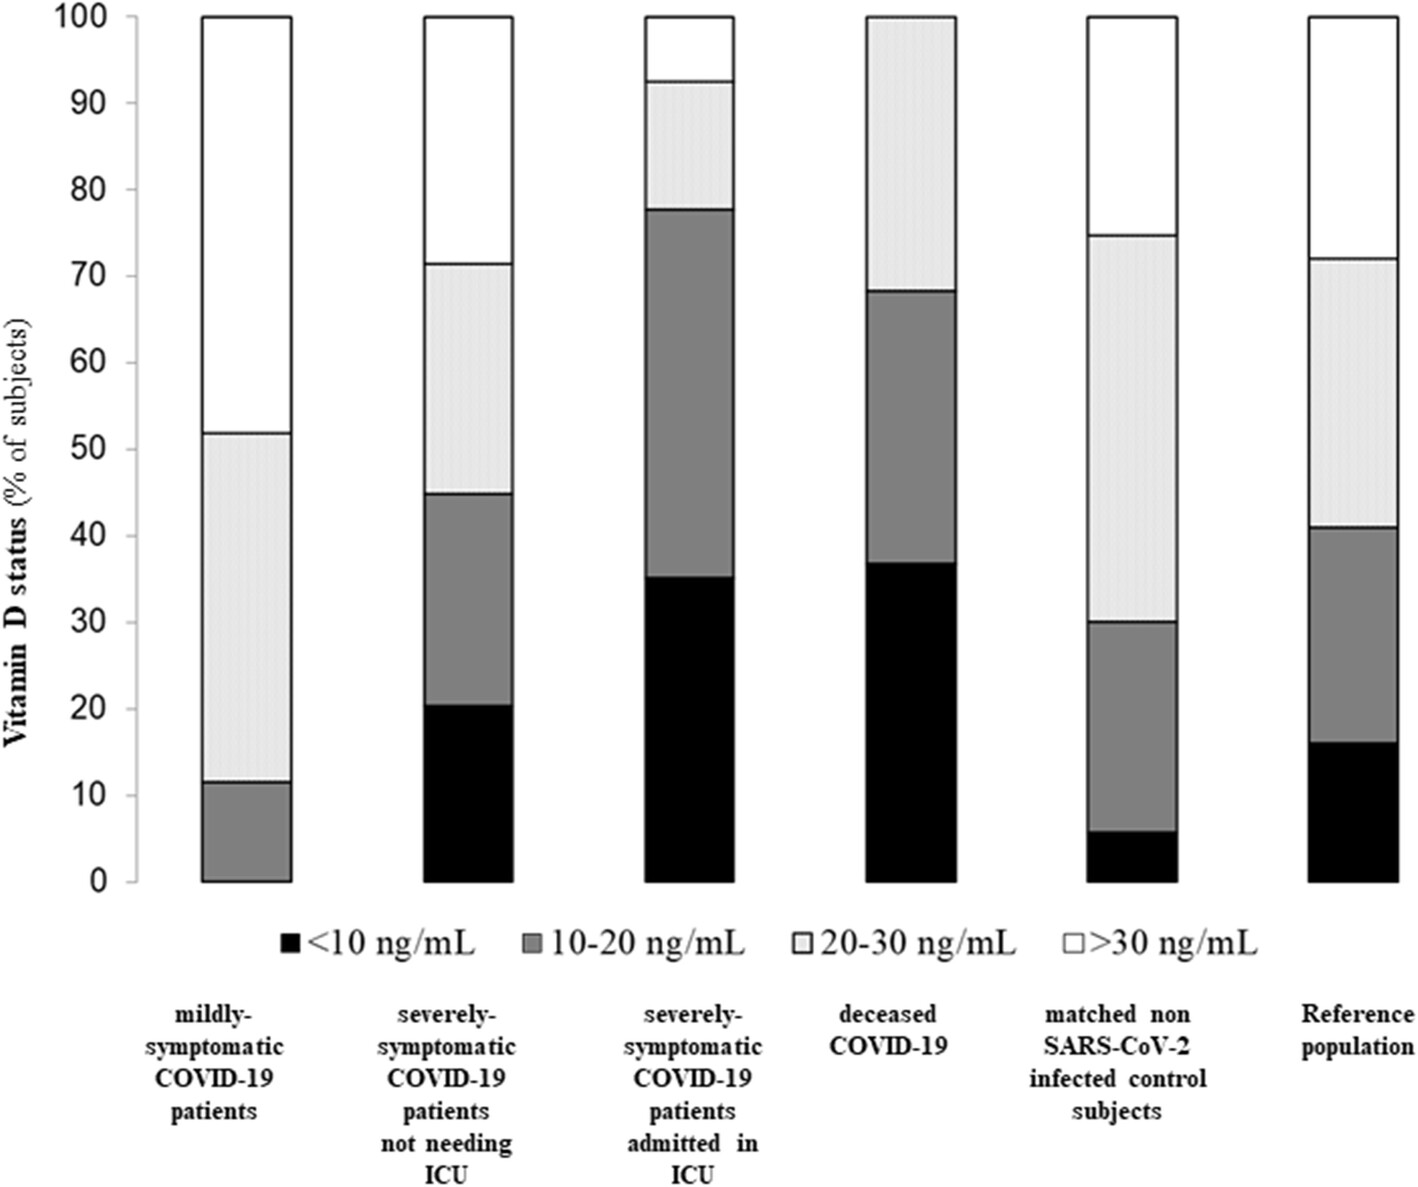
\includegraphics{figures/Campi.2021-Prevalence_rates_of_vitamin_D_insufficiency_or_deficiency.jpg}

}

\caption[Taux de prévalence de l'insuffisance ou de la carence en
vitamine D]{\label{fig-vd-covid-deficiency}Taux de prévalence de
l'insuffisance ou de la carence en vitamine D \autocite{Campi.2021}.}

\end{figure}%

\begin{itemize}
\tightlist
\item
  \textcite{Borsche.2021}: La méta-analyse suggère que la vitamine D
  confère une réduction de l'infection, à une concentration débutant à
  partir de 30 ng/mL, optimale à 55 ng/mL.
\end{itemize}

\section{Etudes observationnelles}\label{etudes-observationnelles}

\begin{itemize}
\item
  \textcite{Oristrell.2022} : Cohorte rétrospective en Espagne de
  108,343 patients, les auteurs ne trouvent pas d'association entre la
  supplémentation en vitamine D. Mais patients \textgreater{} 30 ng/mL =
  baisse de mortalité, sévérité et risque d'infection.
\item
  \textcite{Munshi.2021} : Méta-analyse sur 5 études rétrospective et 1
  étude de cas (2020). N = 376 patients, moyenne = 8.76 ng/mL.
  Standardized mean difference = -0.58 ; On observe de grandes
  différences pour des critères de sévérité (SMD = -0.50) et encore plus
  lors d'admission aux urgences (SMD = -0.84) en particulier.
  Hypovitaminose D associée à un mauvais pronostic pour les patients
  COVID-19.
\item
  \textcite{Campi.2021} : un faible taux de vitamine D est associé à un
  risque accru d'être hospitalisé, d'admission en soins intensifs.
  Plusieurs études associent une déficience sévère (\textless{} 5 ng/mL)
  à un risque accru de mortalité (\Cref{fig-vd-covid-deficiency}).
\item
  \textcite{Pal.2021} : Etude rétrospective sur 72 patients : les
  patients admis à l'hôpital pour un cas de COVID-19 non sévère ont une
  moyenne de 9.8 ng/mL soit une hypovitaminose D (97\% des patients), et
  également une hypocalcémie (67\%).
\item
  Les études écologiques rapportent également une différence de
  concentration de vitamine D entre les patients COVID-19 positifs et
  négatifs (10.8 nmol/L vs 20.8 nmol/L \autocite{Baktash.2021}). En
  effet, il existe une corrélation positive entre l'incidence de
  COVID-19 et le taux de déficience en vitamine D (R = 0.36), la
  fatalité (R = 0.40) et de mortalité (R = 0.38). Le pourcentage médian
  de déficience de vitamine D est de 49\%, indiquant que le 23ème pays
  parmi les 46 pays analysés, possède une déficience en vitamine D de
  49\% \autocite{Mariani.2021}. Une étude d'un centre hospitalier
  rapporte que chez le groupe de patients considéré vitamine D déficient
  (\textless{} 12 ng/mL) contre non déficient (\textgreater{} 12 ng/mL),
  il existe une association entre la déficience de vitamine D et le
  risque de ventilation mécanique invasive et de mortalité (HR = 6.12 et
  14.73 respectivement) \autocite{Radujkovic.2020}.
\end{itemize}

Données contradictoires avec d'autres études observationnelles et RCTs:

- \textcite{Hernández.2020} : 197 patients COVID-19 vs 197 contrôles,
25OHD = 13.8 ng/mL vs 20.9 ng/mL, mais pas d'associations avec la
sévérité ou mortalité. L'étude rétrospective observe néanmoins qu'il
existe une plus grande proportion de patients COVID-19 déficitaires en
vitamine D et corrèle inversement avec la concentration en vitamine D,
rejoignant \textcite{Campi.2021}.

- \textcite{Jevalikar.2021}: 48.2 \% des 410 patients ont un taux de
vitamine D \textless{} 20 ng/mL, mais pas d'association avec la
sévérité, mortalité, admission hospitalière, oxygénothérapie et pas de
corrélation avec les marqueurs inflammatoires (IL-6, CRP).

\begin{itemize}
\tightlist
\item
  \textcite{Wimalawansa.2022} : L'auteur se base sur un risque
  d'infection le plus bas observé pour déterminer un taux de 50 ng/mL,
  en se basant sur deux études prospectives observant l'association
  entre le taux de vitamine D et le risque d'infection nosocomiale,
  mortalité, et durée d'hospitalisation.
\end{itemize}

\section{Effets des interventions thérapeutiques dans la prévention et
le traitement de la
COVID-19}\label{effets-des-interventions-thuxe9rapeutiques-dans-la-pruxe9vention-et-le-traitement-de-la-covid-19}

Globalement, les méta-analyses rapportent une grande hétérogénéité des
essais cliniques ce qui rend les informations moins précises, et plus
difficiles à interpréter, comme par exemple concernant le jour de la
dose d'admission, la dose administrée

Il existe une part d'études rapportant des résultats contradictoires.
Selon \textcite{Pal.2022}: ``Toutefois, il convient de noter que la
plupart de ces études n'ont pas rapporté d'estimations de risque
ajustées pour les résultats cliniques après ajustement des facteurs de
confusion potentiels''.

\textcite{Vanegas-Cedillo.2022} trouve que la vitamine D est
indépendamment associée à la mortalité de la COVID-19 après ajustement
du facteur confondant de la graisse viscérale. \textcite{Borsche.2021},
après ajustement pour les facteurs confondants, arrive à la conclusion
que seul l'âge et la vitamine D sont associés à la mortalité de la
COVID-19.

Malgré des essais cliniques contradictoires, il existe de même une
proportion de méta-analyses et d'études cliniques qui rapportent des
effets bénéfiques de la vitamine D dans la prévention et le traitement
de la COVID-19 \autocite{Pal.2022}.

\subsection{Etudes pré-cliniques}\label{etudes-pruxe9-cliniques}

Le rapport entre le peptide LL-37 et le nombre total de leucocytes
sériques chez les patients atteints de COVID-19 est corrélé avec la
sévérité. Il existe une corrélation entre le CRP, IL‑6, PCT, compte
leucocytaire, LDH et sévérité de la maladie \autocite{Keutmann.2022}. Le
peptide LL-37 est connu comme ayant des propriétés antimicrobiennes
puissantes par le biais d'un mécanisme différent des défensines contre
les virus et les bactéries \autocite{Cutuli.2024}. Des niveaux sériques
plus faibles de LL-37 sont associés à la gravité de la maladie et à la
durée du séjour à l'hôpital \autocite{Keutmann.2022} et il a été observé
que les niveaux de calcidiol sont directement corrélés aux niveaux de
LL-37 chez les patients en sepsis \autocite{Cutuli.2024}.

Les études montrent que les cellules épithéliales pulmonaires expriment
à la fois le \ac{VDR} et la 1α-hydroxylase, ce qui impliquent qu'elles
induisent la production de peptides antimicrobiens, en particulier la
cathélicidine et la défensine β4 \autocite{Cutuli.2024}.

\textcite{Zhang.2012}: Inhibition de la production des cytokines (IL-6,
à partir de 30 ng/mL, testé jusqu'à 70 ng/mL. Dose d'inhibition maximale
à 50 ng/mL, et pas d'effet observé supplémentaire à 70 ng/mL
(\Cref{fig-vd-dose-cytokine}).

\begin{figure}

\centering{

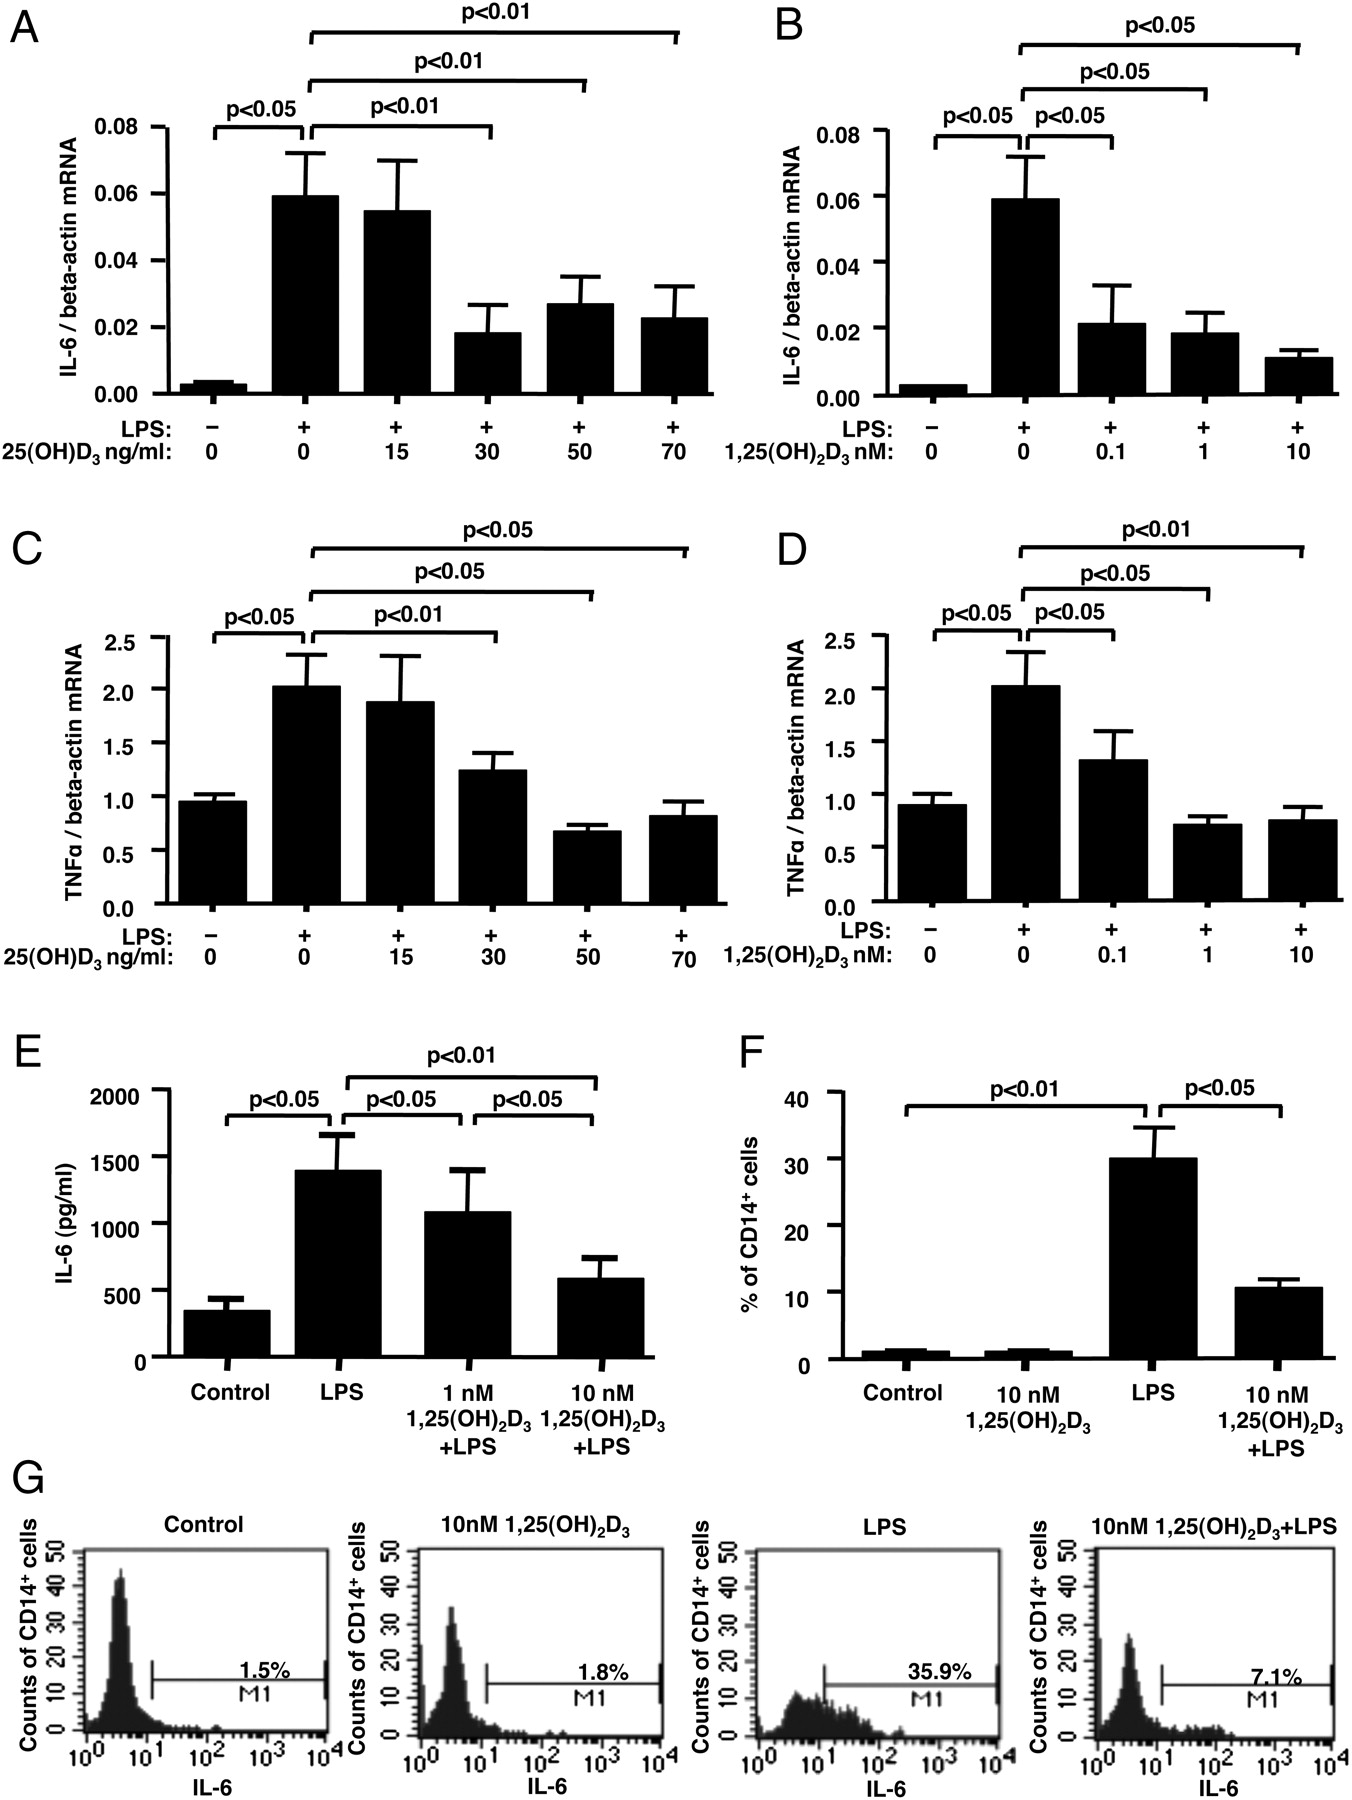
\includegraphics{figures/Zhang.2012-vd_dose_cytokine.jpeg}

}

\caption[Effets de la vitamine D sur la production de
cytokines]{\label{fig-vd-dose-cytokine}\textbf{Effets de la vitamine D
sur la production de cytokines} \autocite{Zhang.2012}.}

\end{figure}%

\subsection{Etudes cliniques}\label{etudes-cliniques}

\begin{itemize}
\tightlist
\item
  Au moins 50 ng/mL de vitamine D nécessaire pour une protection contre
  la COVID-19, selon les méta-analyses. \autocites[
  ]{Borsche.2021}{Wimalawansa.2022}
\end{itemize}

Il existe plusieurs phases de progression de la sévérité de la COVID-19.
L'Organisation Mondiale de la Santé a défini une classification des
phases en fonction de leur sévérité \autocites[
]{WHO.2023.org}{Agarwal.2020} :

\begin{itemize}
\tightlist
\item
  Phase symptomatique légère: Fièvre, toux, fatigue, anorexie,
  essoufflement, myalgie, anosmie, agueusie. Symptômes non spécifiques:
  maux de gorge, congestion nasale, maux de tête, diarrhée, nausées et
  vomissements
\item
  Phase modérée : Définie comme l'absence de critères sévères ou
  critiques. Pneumonie (fièvre, toux, dyspnée, hyperventilation),
  SpO\textsubscript{2} \textgreater{} 90\%
\item
  Phase sévère : Pneumonie, sepsis, SpO\textsubscript{2} \textless{}
  90\%, fréquence respiratoire \textgreater{} 30/min
\item
  Phase critique: \ac{SDRA}, sepsis, choc septique, thrombose aiguë
  nécessitant une ventilation mécanique ou traitement par vasopresseurs
  en unité de soins intensifs.
\end{itemize}

\subsubsection{Etudes en phase hospitalière (visée
curative)}\label{etudes-en-phase-hospitaliuxe8re-visuxe9e-curative}

Généralement dans les études visent à tester l'efficacité de la vitamine
D sur un plan curatif, les patients sont déjà infectés par la COVID-19
et symptomatique et sont administrés une dose unique ou répétée de
vitamine D lors de l'entrée en hospitalisation.

\begin{itemize}
\item
  \textcite{Zhong.2024}: Méta-analyse de 5 RCTs pour une forte dose
  (définie comme une dose unique de ≥100 000 UI ou une dose quotidienne
  de ≥10 000 UI atteignant une dose totale de ≥100 000 UI), analyse ne
  constatant pas d'amélioration de la vitamine D sur la mortalité ou
  admission en soins intensifs.
\item
  \textcite{Ghelani.2021} : Méta-analyse, la vitamine D réduit la
  sévérité et la mortalité (Summary Relative Risk = 0.38 et SRR = 0.35
  respectivement). Plus de réduction observée sur les patients âgés et
  se situant à des latitudes plus élevées.
\item
  \textcite{Borsche.2021}: Méta-analyse en faveur de la vitamine D.
  Forte corrélation inverse de mortalité avec le taux de vitamine D. Les
  auteurs suggèrent également que les taux de vitamine D sont sans
  dangers en prenant en compte les besoins en vitamine K2 ; certains
  répondeurs faibles à la vitamine D devraient avoir une concentration
  augmentée à 75 ou 100 ng/mL pour avoir un effet similaire aux
  répondeurs modérés.
\item
  Selon \textcite{Borsche.2021}, la méta-analyse des 8 études analysées
  rapporte une médiane de 23,2 ng/mL. Les régressions mathématiques de
  deux bases de données séparées montrent que le taux de mortalité
  diminue à partir de 30 ng/mL, et un seuil de 50 ng/mL serait optimal
  pour diminuer la mortalité liée à la COVID-19.
\item
  \textcite{Pal.2022}: Méta-analyse, 10 études observationnelles et 3
  RCTs. La vitamine D réduit la mortalité et le risque d'admission en
  soins intensifs. L'analyse sous-groupe révèle que la supplémentation
  est bénéfique lorsque les patients sont déjà atteints de COVID-19 mais
  pas lorsqu'ils ont déjà reçu de vitamine D avant le diagnostic.
\item
  La méta-analyse rapporte que la vitamine D diminue la mortalité, le
  taux d'admission en soins intensifs et le besoin de ventilation
  mécanique. L'analyse méta-régression impacte l'association entre la
  supplémentation en vitamine D et la mortalité, mais pas le genre,
  l'hypertension, le diabète et ni l'usage de corticostéroïdes
  \autocite{Hariyanto.2022}.
\item
  \textcite{Pal.2022} rapportent également 4 RCTs ou études
  observationnelles qui ne sont pas en faveur de la vitamine D.
\item
  L'étude de \textcite{Kaufman.2020} : Sur 191 779 patients, 39 190
  (12,5\%) sont positifs au COVID-19 avec \textless{} 20 ng/mL, 27 870
  patients (8,5\%) avec 30-34 ng/mL (8,1\%) et 12 321 (5,9\%) patients
  positifs \textgreater= 55 ng/mL Le minimum d'infection est observé
  pour un taux de 55 ng/mL.
\end{itemize}

\autocite{Annweiler.2022} : Etude chez les patients âgés de plus de 65
ans, pas de bras contrôle pour des raisons éthiques médicales (majorité
en hypovitaminose D) : dose unique de 50 000 UI vs 400 000 UI, baisse de
la mortalité 11\% vs 6\% à 14 jours, mais pas à 28 jours.

\begin{itemize}
\tightlist
\item
  L'usage de vitamine D est associée à une réduction du rapport
  neutrophile-lymphocyte périphérique, qui est un paramètre fonctionnel
  associé à une réduction de la mortalité et de passer en soins
  intensifs (3000-6000 UI/j pour 2 mois) \autocite{Maghbooli.2021}
\end{itemize}

RCT contradictoires :

\begin{itemize}
\item
  \textcite{Cereda.2021} : La supplémentation moyenne \textgreater{}
  1800 UI/jour ne donne pas de différence par rapport au groupe non
  supplémenté en terme d'hospitalisation.
\item
  \textcite{Murai.2021} : L'essai clinique ne recommande pas la
  supplémentation en vitamine D. Dose unique de 200 000 UI de vitamine
  D3 vs placebo, n =
\end{itemize}

\begin{enumerate}
\def\labelenumi{\arabic{enumi}.}
\setcounter{enumi}{119}
\tightlist
\item
  Pas de différence significative en terme de durée d'hospitalisation,
  de mortalité, d'admission aux urgences ou de ventilation mécanique.
\end{enumerate}

\subsubsection{Etudes en phase
réanimation}\label{etudes-en-phase-ruxe9animation}

Déficience en soin intensif généralement définie comme calcitriol
\textless{} 12 ng/mL, déficience selon l'IOM est \textless{} 20 ng/mL
\autocite{Cutuli.2024}.

Contexte seul de soin intensif sans COVID-19 : Il est rapporté que 40 -
70 \% des patients en soins intensifs sont déficients en vitamine D. Des
études observationnelles rapportent que la déficience en vitamine D
\textless{} 15 ng/mL est prédictive du risque de sepsis et de mortalité,
93,5\% de déficience dont 53,3\% sont extrêmement bas, à \textless{} 7
ng/mL. Les méta-analyses rapportent que les niveaux bas de vitamine D
sont indépendamment associés à une plus grande mortalité, et en
particulier l'analyse sous-groupe montre que seule la déficience de
vitamine D \textless{} 10 ng/mL est associé à une augmentation de
mortalité, mais que cette association n'est pas retrouvée pour des
niveaux de vitamine D plus élevés \autocite{Cutuli.2024}.

\begin{itemize}
\tightlist
\item
  Seulement deux essais cliniques à large nombre de patients ont examiné
  le rôle de la vitamine D en soins intensifs dans la COVID-19,
  VITdAL-ICU et VIOLET. Pas de conclusions positives, cependant
  l'analyse sous-groupe \textless{} 12 ng/mL révèle une réduction de
  mortalité de chez le groupe vitamine D comparé au placebo (28.6\% vs
  46.1\%) \autocite{Cutuli.2024}. L'étude VIOLET a été prématurément
  arrêtée, et les deux études présentent un niveau bas de sepsis. Il
  existe trois autres études analysés par \textcite{Cutuli.2024} qui
  présentent un effectif plus faible, et ne sont pas conclusives. Selon
  les auteurs, des essais cliniques spécialisés à grande échelle sur la
  question n'ont pas encore été conduits et seraient importants.
\end{itemize}

\textcite{Argano.2023}: Méta-analyse de 5 \acp{RCT} sur la mortalité et
l'admission en soins intensifs, en analysant le risque de biais par la
méthodologie Cochrane ROB 2, avec l'analyse \ac{TSA}
\autocite{Kang.2021}. L'administration de vitamine D résulte en une
réduction de la mortalité et de l'admission en soins intensifs (SMD:
(95\% CI): 0.49 (0.34--0.72) et 0.28 (0.20--0.39)). L'analyse TSA révèle
que le nombre de patient est suffisant pour arriver à une conclusion
concernant la réduction de l'admission en soins intensifs, mais que
l'association positive du facteur protecteur de la vitamine D sur la
mortalité nécessite encore des études supplémentaires.

\begin{itemize}
\item
  Méta-analyse: \textcite{Pal.2022} : Les auteurs rapportent que la
  vitamine D est efficace pour améliorer les résultats cliniques, et en
  particulier lorsque la vitamine D est utilisée après l'infection.
\item
  \textcite{Karonova.2022.pharmaceuticals}: 321 patients, prévalence de
  patients sévères chez les patients déficients en vitamine D. Analyse
  ROC révèle un niveau de 11,4 ng/mL associé à la mortalité ; -
  \textless11,4 ng/mL : Th CD3+ CD4+ diminué - Tfh diminué dans les deux
  groupes - \textgreater{} 11,4 ng/mL : Augmentation Th2 central memory
  et diminution Th17 central memory \{Lien avec observation du rôle
  pathologique de Th17, et IL-17 dans l'inflammation, diminué lors de
  l'administration de vitamine D\} \autocites[ ]{Pacha.2020}[
  ]{Raucci.2020}[ ]{Gilani.2022}{Cutuli.2024}
\item
  \textcite{Rastogi.2022} : SHADE study: RCT, 40 patients, 60 000 UI de
  vitamine D3 vs placebo, 1 dose, 7 jours. Objectif \textgreater{} 50
  ng/mL. n = 16 vitD vs n = 24. Résultats: 10 patients vs 5 contrôles
  sont RNA négatif. Fibrinogène faiblement diminué.
\item
  \textcite{Leaf.2014} : Calcitriol n'augmente pas le niveau de
  cathélicidine en sepsis et effets mixtes sur les autres marqueurs
  immunologiques. Dose = 2 µg en IV = 80 UI {[}ce qui semble extrêmement
  bas{]}.
\end{itemize}

\section{Discussion}\label{discussion}

\begin{itemize}
\item
  Il existe de multiples méta-analyses, et essais cliniques randomisés,
  montrant une efficacité de la vitamine D en ce qui concerne un usage
  en prévention, curatif ou même dans un cadre critique nécessitant le
  passage en unité de soin intensif.
\item
  La vitamine D possède un rationnel thérapeutique notable, agissant sur
  plusieurs niveaux dans la physiopathologie du COVID-19 : elle agit sur
  la tempête cytokinique, le SRAA, module l'inflammation et possède une
  action indirecte antivirale par l'induction de cathélicidine.
\item
  Malgré cela, il existe également des études montrant l'absence d'effet
  de la vitamine D ce qui rend incertain la place de la vitamine D dans
  l'arsenal thérapeutique de la COVID-19. Les études présentent une
  grande variabilité concernant la méthodologie, la dose employée, et le
  moment de l'administration de la vitamine D, ce qui augmente
  l'hétérogénéité des résultats et l'incertitude de l'efficacité de la
  vitamine D. Même lors des essais cliniques à grand nombre de patients,
  les résultats ne sont pas tout le temps positifs. La méta-analyse de
  \textcite{Zhong.2024} sur 5 essais cliniques ne supporte pas l'usage
  d'une dose unique élevée de vitamine D dans un cadre curatif.
\item
  Selon le rationnel physiologique de l'effet de la vitamine D,
  l'hétérogénéité des résultats peut s'expliquer par la dose
  d'administration pouvant être insuffisante pour atteindre une dose
  jugée optimale d'au moins 30 ng/mL et idéalement 50 ng/mL où le taux
  d'infection et la mortalité seraient les plus basses
  \autocites{Wimalawansa.2022}[ ]{Kaufman.2020}{Borsche.2021}. De plus
  comme la vitamine D n'est pas un médicament mais un nutriment, il
  existe une grande variabilité dans l'absorption de la vitamine D, qui
  peut être influencée par la nutrition, et la variabilité d'absorption
  et de distribution de la concentration de calcidiol qui est notamment
  dépendante du poids \autocite{Ekwaru.2014}, ainsi que de la
  variabilité génétique de réponse au VDR. Ainsi, \textcite{Vukić.2015}
  ont déterminé qu'il existait deux groupes de répondeurs à la vitamine
  D en fonction du nombre de pourcentage de gène activés, qui peut aller
  de 33\% pour les répondeurs les plus bas à 80\% chez les forts
  répondeurs. La variabilité de la réponse à la vitamine D entre
  patients est donc potentiellement très élevée, et la concentration
  plasmatique atteinte entre chaque patient pour une même dose de
  vitamine D peut être très variable.
\item
  L'administration de vitamine D à visée curative pour une dose de 5000
  UI/j est trop lente pour élever la concentration plasmatique de
  calcidiol car la métabolisation de la vitamine D nécessite plusieurs
  mois avant d'atteindre une concentration supérieure à 30 ng/mL
  \autocite{Mocanu.2009}. Ainsi \textcite{Wimalawansa.2022} propose une
  dose de charge élevée de vitamine D ou bien une dose bolus de
  calcidiol oral qui serait rapidement absorbée par l'organisme, afin de
  pouvoir rapidement élever la concentration de calcidiol à atteindre en
  quelques jours ou heures respectivement. Une dose bolus de 100 000 UI
  est suffisante pour atteindre des doses \textgreater20 ng/mL mais une
  dose de 300 000 UI est nécessaire pour atteindre une concentration
  \textgreater{} 30 ng/mL de calcidiol \autocite{Kearns.2014}
\item
  L'essai clinique de \textcite{Murai.2021}, considéré comme de bonne
  qualité méthodologique par \textcite{Annweiler.2021} et
  \textcite{Argano.2023}, selon les lignes directrices de
  \textcite{Heaney.2014} : en effet, le raisonnement classique de la
  supplémentation en vitamine D n'est pas équivalent à d'autres
  médicaments, car les suppléments ne sont pas la seule source de
  vitamine D, et de plus, il n'y a pas de relation dose-dépendante
  {[}?{]}. L'étude de \textcite{Murai.2021} échappe à 5 pièges de
  méthodologies des \acp{RCT}:
\end{itemize}

\begin{enumerate}
\def\labelenumi{\arabic{enumi})}
\tightlist
\item
  Dose de charge pour remplir le stockage
\item
  Pas de traitement long terme pour maintenir le taux de vitamine D
\item
  L'adhérence au traitement est élevée
\item
  L'augmentation de la concentration de vitamine D est vérifiée après
  supplémentation
\item
  Il est peu probable que le groupe de contrôle ne reçoit pas de
  supplémentation en vitamine D car il est hospitalisé par la même unité
  de recherche.
\end{enumerate}

\autocite{Leaf.2021,Annweiler.2021} : l'étude de \textcite{Murai.2021}
n'a pas suffisamment de puissance, et les patients avec sévérité grave
de la maladie sont exclus, ce qui pourrait expliquer l'absence de
différence significative entre les groupes. Seul la moitié des patients
sont déficients \textless20 ng/mL et seul un quart est en déficience
sévère \textless12 ng/mL. De plus, l'utilisation de la longueur de
séjour à l'hôpital comme critère principal est critiquable, pouvant être
influencée par d'autres facteurs comme le soutien social disponible au
domicile, et ne reflétant pas la sévérité de la maladie
\autocite{Annweiler.2021}, il aurait été préférable d'utiliser d'autres
critères de mesure de la mortalité, ou de la sévérité du COVID-19.

\begin{itemize}
\item
  \textcite{Heaney.2014} propose des lignes directrices méthodologiques
  concernant les essais cliniques pour les nutriments, où la
  méthodologie actuelle est adaptée pour les médicaments pharmaceutiques
  mais inadaptée pour les nutriments car les sources d'apports du
  nutriments sont diverses et que la relation dose-réponse entre la dose
  et un objectif de santé est non linéaire
  \autocite{Grant.2022.nutrients}. Les essais cliniques devraient être
  basés sur la concentration en calcidiol plasmatique initiale et celle
  à atteindre et non pas en dose de vitamine D étant donné la grande
  hétérogénéité observée entre l'administration d'une dose de vitamine D
  et la concentration plasmatique obtenue
  \autocite{Grant.2022.nutrients}.
\item
  Selon \textcite{Grant.2022.nutrients}, les RCTs sur la vitamine D dans
  un contexte général ont échoué car elles se concentrent sur la dose
  plutôt que la concentration, ont donné des doses basses de vitamine D
  qui ne peuvent pas permettre d'atteindre une concentration désirée,
  ont impliqué des patients au-delà de la moyenne de la population, et
  qu'il existe différents niveaux pour différents bénéfices de la santé.
  Les RCTs, et études de randomisation mendéliennes analysent de manière
  limitée les résultats car elles ne prennent pas en compte les effets
  non linéaires de la vitamine D ainsi que la haute variance des dosages
  de vitamine D \autocite{Grant.2022}.
\end{itemize}

\newpage{}

\chapter{Conclusion}\label{conclusion}

\newpage{}

\hypertarget{Bibliographie}{%
\chapter*{\centering Bibliographie}\label{Bibliographie}}
\addcontentsline{toc}{chapter}{Bibliographie}
\singlespace

\printbibliography[heading=none]




\end{document}
